\documentclass[a4paper]{article}
\usepackage[a4paper, total={170mm,257mm}, left=20mm, top=20mm]{geometry}
\usepackage[english]{babel}
\newcommand\hmmax{0}
\newcommand\bmmax{0}
\usepackage{mathtools}
\usepackage{mathrsfs}
\usepackage{amsthm}
\usepackage{amsmath, zref-savepos}
\usepackage{amsfonts}
\usepackage{graphicx}
\usepackage{float}
\usepackage{thmtools}
\usepackage{caption}
\usepackage{subcaption}
\usepackage{amssymb}
\usepackage{placeins}
\usepackage{relsize}
\usepackage{MnSymbol}
\usepackage{nameref}
\usepackage{hyperref}
\usepackage{marvosym}
\usepackage{lipsum}
\usepackage{paralist}
\usepackage{wasysym}
\usepackage{multirow}
\usepackage{auto-pst-pdf}
\usepackage{ulem}
\usepackage{minted}
\usepackage{fancyref}
\usepackage{xfrac}
\usepackage[autostyle]{csquotes}
\usepackage{bm}
\usepackage{extarrows}
\usepackage{booktabs}
\usepackage{multirow}
\usepackage{bookmark} %faster updated bookmarks
\usepackage{wrapfig}
\usepackage{xfrac}
\usepackage{mathtools}
\usepackage{xcolor,cancel}
\usepackage{centernot}
\usepackage{enumitem}
\usepackage{cleveref}
\usepackage{lscape}
\usepackage{longtable}
\usepackage{nth}
\usepackage{tikzsymbols}
\usepackage{rotating}
\usepackage[gen]{eurosym}
\usepackage{hhline}

%%%%%%%%%%%%%%%
\restylefloat{figure}
\newtheorem*{conthm}{Monotonic Sequence Theorem}
\newcommand{\diff}{\mathrm{d}}
\newcommand{\bd}{\mathrm{bd}\,}
\newcommand{\cl}{\mathrm{cl}\,}
\newcommand{\ext}{\mathrm{ext}\,}
\newcommand{\intr}{\mathrm{int}\,}
\newcommand{\vbrac}[1]{\left\vert #1\right\vert}
\newcommand{\brac}[1]{\left( #1\right)}
\newcommand{\cbrac}[1]{\left\{ #1\right\}}
\newcommand{\sbrac}[1]{\left[ #1\right]}
\newtheorem{solution}{Solution}
\declaretheorem[name=Solution, refname={Solution,Solutions}, Refname={Solution,Solutions}, style=remark, unnumbered]{sol}
\newcommand{\N}{\mathcal{N}}
\DeclareMathOperator{\var}{Var}
\DeclareMathOperator{\Cov}{Cov}
\newcommand{\cov}[1]{\Cov{\brac{#1}}}
\DeclareMathOperator{\E}{\mathbb{E}}
\DeclareMathOperator{\SE}{\mathbb{SE}}
\DeclareMathOperator{\PP}{\mathbb{P}}
\DeclareMathOperator{\diag}{diag}
\DeclareMathOperator{\rank}{rank}
\DeclareMathOperator{\tr}{tr}
\newcommand{\pr}[1]{\PP{\brac{#1}}}
\newcommand{\given}[2]{\PP{\left( #1 \left| #2 \right) \right. }}
\allowdisplaybreaks
\renewcommand{\theequation}{\arabic{equation}}
\newcommand\ind{\protect\mathpalette{\protect\independenT}{\perp}}
\def\independenT#1#2{\mathrel{\rlap{$#1#2$}\mkern2mu{#1#2}}}
\newcommand\Ccancel[2][black]{\renewcommand\CancelColor{\color{#1}}\cancel{#2}}
%\numberwithin{equation}{subsection}

%%%LISTS%%%
\setlist[enumerate]{
	align=left,
    leftmargin=*,
    itemindent=*, 
    labelsep=*, 
    labelwidth=*
}
\setlist[itemize]{
	align=left,
    leftmargin=*,
    itemindent=*, 
    labelsep=*, 
    labelwidth=*
}

%%%PLOTS%%%
\usepackage{pgfplots}
\pgfplotsset{compat=newest}
\usepgfplotslibrary{statistics}
\usepgfplotslibrary{fillbetween}
\pgfmathdeclarefunction{gauss}{2}{\pgfmathparse{1/(#2*sqrt(2*pi))*exp(-((x-#1)^2)/(2*#2^2))}}
%%%%%%%%%%%%%

%%%DIAGONAL MATRICES%%%
\newcommand{\diagentry}[1]{\mathmakebox[1.8em]{#1}}
\newcommand{\xddots}{%
  \raise 4pt \hbox {.}
  \mkern 6mu
  \raise 1pt \hbox {.}
  \mkern 6mu
  \raise -2pt \hbox {.}
}
%%%%%%%%%%%%%%%%%%%%%%%

%%%ROTATE IN TABLES%%%
\newcommand{\STAB}[1]{\begin{tabular}{@{}c@{}}#1\end{tabular}}
%%%%%%%%%%%%%%%%%%%%%%


\title{Course summary}

\author{Stephanie Ranft S2459825}

\date{\parbox{\linewidth}{\centering%
  \today\endgraf\bigskip
  \textbf{Statistics 1B \\ PSBE1-09}}}
\clearpage

\begin{document}
\maketitle
\section{Overview}
\begin{enumerate}[label=\textbf{\S~\arabic*}, ref=\S~\arabic*]
\setcounter{enumi}{4}
    \item Statistical inference: estimation
    \begin{enumerate}[label=\textbf{\S~5.\arabic*}, ref=\S~5.\arabic*]
        \item Point and interval estimation
        \begin{itemize}
            \item \textit{Point estimate}: estimates a parameter with a single number, e.g. $\Bar{x}$ is a point estimate of $\mu$.
            \item \textit{Interval estimate}: estimates a parameter with a range, e.g. confidence interval $\Bar{x} \pm z^* \sigma/\sqrt{n}$ is an interval estimate of $\mu$. 
            \item \textit{Confidence interval} = point estimate $\pm$ margin of error. The confidence level comes from: the probability that the estimate is within $z^*_{1 - \alpha/2}$ standard errors from the parameter is equal to $(1-\alpha)\%$, e.g. the probability that $\Bar{x}$ is in the range $(\mu - 1.96 \times \sigma/\sqrt{n}, \mu+ 1.96 \times \sigma/\sqrt{n})$ is 95\%. 
            \begin{itemize}
                \item In the long run, $(1-\alpha)\%$ of such intervals would contain the parameter.
                \item With repeated sampling, there is a $(1-\alpha)\%$ chance that a random confidence interval will cover the true parameter value. 
                \item $(1-\alpha)\%$ percent of the time (in repeated sampling from the same population) the parameter will lie in the range of the confidence interval.
            \end{itemize}
            \item \textit{Margin of error} = critical statistic ($z^*$ or $t^*$, for e.g.) $\times$ standard error of the point estimate. As the sample size increases, the standard error of the estimate decreases and thus so does the margin of error.
            \item \textit{Unbiased estimate}: the expected value of the point estimate is equal to the parameter - another way to write it is $\text{Bias}\brac{\Bar{x}} = \mu - \E \brac{\Bar{x}}$. An estimator is unbiased if the bias equals zero. Recall: the expected value is basically the mean.
            \item \textit{Efficient estimator}: an unbiased estimator which has a small standard error (relatively speaking) is also efficient. You can Google the Cramer-Rao inequality if you have interest, but it is not pertinent to this course. For example, $\Bar{x}$ is efficient but $Q_2$ is not.
            \item \textit{Notation}: $\hat{\phantom{\mu}}$ over a parameter denotes an estimator of the parameter, e.g. $\hat{\mu}$ estimates $\mu$.
            \item \textit{Central Limit Theorem (CLT)}: due to the \textit{Law of Large Numbers (LLN)}, as the sample size increases the estimate tends towards the parameter which is seen by the decreasing standard error.
        \end{itemize}
        
        \item Confidence interval for a proportion
        \begin{itemize}
            \item \textit{CI for proportion $\pi$}: \[
            \hat{\pi} \pm z^*_{1-\alpha/2} \times se_{\hat{\pi}} , \quad \text{where } se_{\hat{\pi}} = \sqrt{\frac{\hat{\pi}\brac{1 - \hat{\pi}}}{n}}.
            \]
        \end{itemize}
        
        \item Confidence interval for a mean:
        \begin{itemize}
            \item \textit{CI for mean $\mu$}: 
            \[
            \bar{x} \pm z^*_{1-\alpha/2} \times \frac{\sigma}{\sqrt{n}} , \quad \text{where $\sigma$ is known.}
            \]
            \[
            \bar{x} \pm t^*_{1-\alpha/2, \text{ df}} \times \frac{s}{\sqrt{n}} , \quad \text{where $\sigma$ is unknown.}
            \]
            $t^*_{1-\alpha/2, \text{ df}}$ is larger than $z^*_{1-\alpha/2}$ to account for the additional error introduced by using $s$ to estimate $\sigma$ for the standard error. They are equal for ``infinite sample sizes'', or near equal for very large sizes.
            \item \textit{Robustness}: a method is robust if it performs well despite violations of certain assumptions, e.g. normality. This is important from the book: \textit{...the confidence interval for a mean using the $t$ distribution is robust against violations of the normal population assumption. Even if the population is not normal, confidence intervals based on the $t$ distribution still work quite well, especially when $n$ exceeds about 15. As the sample size gets larger, the normal population assumption becomes less important, because of the Central Limit Theorem. The sampling distribution of the sample mean is then bell shaped even when the population distribution is not. The actual probability that the 95\% confidence interval method contains $\mu$ is close to 0.95 and gets closer as $n$ increases. \newline An important case when the method does not work well is when the data are extremely skewed or contain extreme outliers. Partly this is because of the effect on the method, but also because the mean itself may not then be a representative summary of the centre.} This last part refers to using the median or the mode to summarise the centre, instead of the mean, because of skew.
        \end{itemize}
        
        \item Choice of sample size
        \begin{itemize}
            \item \textit{Limiting the margin of error for a certain confidence level}: suppose you want to ensure that the margin of error is less than (or equal to) some value, say $A$, with probability $\brac{1 - \alpha}\%$ then you need to alter the sample size, e.g.
            \begin{align*}
                \underbrace{\overbrace{z^*_{1 - \alpha/2}}^{\text{critical value}} \times \overbrace{\frac{\sigma}{\sqrt{n}}}^{\text{standard error}}}_{\text{margin of error}} &\leq A & &\iff & n &\geq \brac{z^*_{1 - \alpha/2} \times \frac{\sigma}{A}}^2.
            \end{align*}
            This works with any standard error formula (e.g. using $\sigma$ or $s$) and any critical value (e.g. $z^*_{1 - \alpha/2}$ or $t^*_{1 - \alpha/2, \text{ df}}$); just rearrange to solve for $n$.
        \end{itemize}
        
        \item Estimation Methods: Maximum Likelihood and the Bootstrap
        \begin{itemize}
            \item From the book: \textit{For point estimation, Fisher proposed the maximum likelihood estimate. This estimate is the value of the parameter that is most consistent with the observed data, in the following sense: If the parameter equalled that number (i.e., the value of the estimate), the observed data would have had greater chance of occurring than if the parameter equalled any other number.} 
            \item Also: \textit{In fact, with random sampling, the maximum likelihood estimate of a population proportion is necessarily the sample proportion.}
            \item \textit{Maximum likelihood estimator (MLE)}: is the most efficient for large enough samples, consistent (bias diminishes to zero as $n$ increases), and have approximately normal sampling distribution. This normality of the sampleing distribution allows us to compute confidence intervals. 
            \item $\bar{x}$ is the MLE for $\mu$, as the standard error for $Q_2$ is $1.25 \sigma /\sqrt{n}$, which is more than the standard error for $\bar{x}$.
            \item \textit{Bootstrap method}: treat the sampling distribution as if it is the population distribution, e.g. $\bar{X}\sim \N \brac{\mu, \sigma/\sqrt{n}}$ is the sampling distribution of the mean. Then take $n$ samples (with replacement) from the sampling distribution, and compute the mean. Do this about 1000 times, and the means of the means will be near the parameter value for the population. (See the simulation \url{http://onlinestatbook.com/stat_sim/sampling_dist/index.html}.)
        \end{itemize}
    \end{enumerate}
    
    \item Statistical Inference: Significance Tests
    \begin{enumerate}
        \item The five parts of a significance test
        \begin{itemize}
            \item \textit{Hypothesis}: a predictive statement about a parameter that can be tested. The null hypothesis always corresponds to ``no difference'', ``no effect'' or ``no association'' to protect society from any dramatic changes (Type I errors). The alternative is the converse of the null hypothesis, or the research hypothesis - if ``no effect'' then what we expect. We do not ``accept'' either, we only choose to ``reject'' or ``not reject'' the null hypothesis.
            \item \textit{Significance test}: uses sample data to summarise evidence about a hypothesis.
            \item The five parts are: assumptions, hypotheses, test statistic, $p$-value, and conclusion.
            \item \textit{Test statistic}: summary statistic used in significance test, e.g. $z$-value or $t$-value.
            \item \textit{$p$-value}: the probability of achieving a test statistic equal to or more extreme than that which we observed, e.g. $\pr{\vbrac{Z}>z} = p$ (two-tailed $H_a$), $\pr{Z>z}=p$ (right-tailed $H_a$) or $\pr{Z<z}=p$ (left-tailed $H_a$). The smaller the $p$-value, the greater the evidence against $H_0$ and thus for rejecting it. We decide to reject for $p< \alpha$, where $\alpha$ is our accepted probability of a Type I error.
            \item \textit{$\alpha$-level}: if you decrease $\alpha$, the critical value $z^*$ or $t^*$ increases. The converse is also true. $\alpha$ is the probability of a Type I error.
        \end{itemize}
        
        \item Significance test for a mean
        \begin{itemize}
            \item \textit{Assumptions:} random sampling and parameter is normally distributed.
            \item \textit{Hypotheses:} $H_0$: $\mu=\mu_0$ and $H_a$: $\mu \ne \mu_0$ for two-sided, $\mu>\mu_0$ for right-tailed or $\mu<\mu_0$ for left-tailed.
            \item \textit{Test statistic:} $z$-value for $\sigma$ in the population known, or $t$-value for $\sigma$ in the population unknown.
            \begin{align*}
                z &= \frac{\bar{x} - \mu_0}{\sigma/\sqrt{n}} \sim \N \brac{0,1}. \\
                t &= \frac{\bar{x} - \mu_0}{s/\sqrt{n}} \sim t \brac{\text{df}=n-1}.
            \end{align*}
            \item \textit{$p$-value}: probability of observing a test statistic at least or more extreme (in the direction of $H_a$). 
            \item \textit{Conclusion}: reject $H_0$ if $p<\alpha$ and assumptions are met.
        \end{itemize}
        
        \item Significance test for a proportion
        \begin{itemize}
            \item \textit{Assumptions:} random sampling and sampling distribution of estimate is approximately normal. The latter implies that $n \Hat{\pi}$ and $n \brac{1 - \Hat{\pi}}$ must both be at least 10.
            \item \textit{Hypotheses:} $H_0$: $\pi=\pi_0$ and $H_a$: $\pi \ne \pi_0$ for two-sided, $\pi>\pi_0$ for right-tailed or $\pi<\pi_0$ for left-tailed.
            \item \textit{Test statistic:} 
            \begin{align*}
                z &= \frac{\Hat{\pi} - \pi_0}{se_0} \sim \N \brac{0,1}; &
                se_0 &= \sqrt{\frac{\pi_0 \brac{1 - \pi_0}}{n}}.
            \end{align*}
            \item \textit{$p$-value}: probability of observing a test statistic at least or more extreme (in the direction of $H_a$). 
            \item \textit{Conclusion}: reject $H_0$ if $p<\alpha$ and assumptions are met.
        \end{itemize}
        
        \item Decisions and types of errors in tests
        \begin{itemize}
            \item \textit{Type I error}: probability of incorrectly rejecting the null hypothesis, $\alpha$. ($H_0$ is true in reality.)
            \item \textit{Type II error}: probability of incorrectly not rejecting the null hypothesis, $\beta$. ($H_a$ is true in reality.)
            \item \textit{Power}: probability of correctly rejecting the null hypothesis, $1-\beta$. ($H_a$ is true in reality.)
            \item \textit{Sensitivity}: probability of correctly not rejecting the null hypothesis, $1-\alpha$. ($H_0$ is true in reality.)
            \item $alpha$ and $\beta$ are inversely proportional, meaning that a decrease in $\alpha$ results in an increase in $\beta$, and vice-versa. Recall that power is $1 - \beta$, so decreasing $\alpha$ decreases the power of your test. 
            \item If the test statistic is in the rejection region, then $p<\alpha$ and the hypothesised parameter value, e.g. $\mu_0$, is not included in the confidence interval of the same $\alpha$ level.
        \end{itemize}
        
        \item Limitations of significance tests
        \begin{itemize}
            \item \textit{Statistical vs. practical significance}: a small $p$-value only signifies that the probability, under the null hypothesis, of observing a test statistic as or more extreme is very small. This does not give any indication of the true value of the parameter. Confidence intervals are ``better'' in the sense that they do give an indication of the true value of the parameter.
            \item \textit{Effect size}: used to summarise practical significance, e.g. indicates how likely a researcher is observe an effect. Cohen's $d$ gives the $z$-value, which should be at least 0.8 to have a large effect; medium is around 0.5 and small is $\leq 0.2$.
            \item Read page 173.
        \end{itemize}
        
        \item \textit{Finding $\mathbb{P}$(Type II error)}
        \begin{itemize}
            \item Calculate the cut-off value, i.e. the sample statistic for which you would reject $H_0$, e.g. $\bar{x}>\mu_0 + z^*\times \sigma/\sqrt{n}$ is the cut-off value for a right-tailed hypothesis test.
            \item Use the cut-off value to calculate the $z$-value using $\mu=\mu_a$, where $\mu_a$ is the true parameter value (not $H_0$), e.g.
            \begin{align*}
                z &= \frac{\sbrac{\mu_0 + z^*\times \sigma/\sqrt{n}} - \mu_a}{\sigma/\sqrt{n}} = \frac{\mu_0 - \mu_a}{\sigma/\sqrt{n}} + z^*.
            \end{align*}
            \item Compute the $p$-value, e.g. $p=\pr{Z>z}$ where $z$ was calculated above. This $p$-value is the probability of a Type II error.
            \item $1 -p$-value gives you the power. 
        \end{itemize}
        
        \item Small-sample test for a proportion— the Binomial distribution
        \begin{itemize}
            \item $X \sim \mathcal{B}in(n,p)$ is the probability distribution of ``success'' with probability $p$ and $n$ trials, and $\pr{X=k}$ is the probability of $k$ ``successes''. 
            \begin{align*}
                \pr{X=k} &= \binom{n}{k} p^k (1-p)^{n-k} = \frac{n!}{k!\brac{n-k}!} p^k (1-p)^{n-k}
            \end{align*}
            $\Hat{p}$ estimates $p$ and can be written at $x/n$, where $x$ is the number of successes in a sample of size $n$. 
            \item The mean is $np$ and the standard deviation is $\sqrt{np(1-p)}$. 
            \item If the expected frequencies for both success and failure, $np$ and $n(1-p)$, are both greater than 10, then you can approximate using the \textit{Normal approximation to the Binomial distribution}, $X \sim \N \brac{\mu=np, \sigma=\sqrt{np(1-p)}}$.
        \end{itemize}
    \end{enumerate}
    
    \item Comparison of two groups
    \begin{enumerate}[label=\textbf{\S~7.\arabic*}, ref=\S~7.\arabic*]
        \item Preliminaries for comparing groups
        \begin{itemize}
            \item \textit{Response variable}: the dependent variable, usually the $y$ values is $(x,y)$ bivariate data sets. 
            \item \textit{Explanatory variable}: the independent variable, usually the $x$ values is $(x,y)$ bivariate data sets. 
            \item \textit{Longitudinal study}: same subjects but testing at 2 or more time periods. Usually you compare the difference. Also called matched pairs or dependent sample. 
            \item Read for yourself from page 193 about \textit{cross-sectional studies}, \textit{experimental studies}, \textit{experimental} vs. \textit{control group}, etc.
            \item If two estimates from independent samples have standard errors $se_1$ and $se_2$, then the sampling distribution of their difference has the estimated standard error $\sqrt{se_1^2 + se_2^2} = \sqrt{s_1^2/n_1 + s_2^2/n_2}$.
            \item \textit{Ratios}: if the ratio of two values equals 1, then they are equal, e.g. if the ratio of sample means is $11.9/8.3=1.43$ then one of the sample means is 1.43 times the other. Can be used for effect size.
        \end{itemize}
        
        \item Categorical data: comparing two proportions
        \begin{itemize}
            \item If you have two populations with proportions $\pi_1$ and $\pi_2$ and you calculate the sample proportions $\Hat{\pi}_1$ and $\Hat{\pi}_2$, the sampling distribution of their difference is Normal with mean $\pi_2 - \pi_1$ and variance $\Hat{\pi}_1\brac{1 - \Hat{\pi}_1}/n_1 + \Hat{\pi}_2\brac{1 - \Hat{\pi}_2}/n_2$ (take the square root of the variance for the standard error). We estimate $\pi_2 - \pi_1$ with $\Hat{\pi}_1 - \Hat{\pi}_2$.
            \item \textit{Confidence interval for difference of proportions}: 
            \begin{align*}
                \brac{\Hat{\pi}_1 - \Hat{\pi}_2} \pm z^*_{1 - \alpha/2} \times se; && se &= \sqrt{\frac{\Hat{\pi}_1\brac{1 - \Hat{\pi}_1}}{n_1} + \frac{\Hat{\pi}_2\brac{1 - \Hat{\pi}_2}}{n_2}}.
            \end{align*}
            If the confidence interval contains zero, then you cannot reject the claim that the proportions are the same. This inference depends on the standard error, of course, as a large standard error would indicate that there is a lot of error associated with the estimate. If zero is in the CI, then the lower bound must be \textit{negative} and the upper bound must be \textit{positive}.
            \\
            If the CI contains only negative values then we infer that $\pi_2<\pi_1$, and conversely if the CI contains only positive values then we infer that $\pi_2>\pi_1$.
            \item \textit{Hypothesis testing}: we assume that there is not difference; $H_0$: $\pi_1 = \pi_2$, $\pi = \pi_2 - \pi_1=0 = \pi_0$.
            \begin{align*}
                \Hat{\pi} &= \frac{\Hat{\pi}_1 n_1 + \Hat{\pi}_2 n_2}{n_1 + n_2} = \frac{\sum x_1 + \sum x_2}{n_1 + n_2},
                \shortintertext{where $x_1$ is the sum of successes in sample 1, and similarly for $x_2$ - it is the sum of successes in sample 2.}
                \implies z &= \frac{\brac{\Hat{\pi}_2 - \Hat{\pi}_1} - \pi_0}{se_0} = \frac{\Hat{\pi}_2 - \Hat{\pi}_1}{se_0}; \\ 
                se_0 &= \sqrt{\Hat{\pi} \brac{1-\Hat{\pi}}\brac{\frac{1}{n_1} + \frac{1}{n_2}}}.
            \end{align*}
        \end{itemize}
        \clearpage
        \item Quantitative data: comparing two means
        \begin{itemize}
            \item \textit{Confidence interval for the difference in means}: for independent random samples from two normally distributed populations, the CI for $\mu_2 - \mu_1$ is
            \begin{align*}
                \brac{\bar{y}_2 - \bar{y_2}} \pm t^*_{1 - \alpha/2, \text{ df}=n_1+n_2-2} \times se; && se &= \sqrt{\frac{s_1^2}{n_1} + \frac{s_2^2}{n_2}}.
            \end{align*}
            This method is robust to violations of the normal assumption provided that $n\geq 30$ because of the CLT. Beaware of extreme outliers or extreme skew which may nullify the robustness for $n\approx 30$.
            \\
            Similar to the inference about proportions, you want that zero is in the interval and if not, then at least you can infer that one group has a higher mean than the other.
            \\
            In this case, we don't assume equal variance in the populations (homoskedasticity).
            \item \textit{Significance tests are differences in means}: we claim that there is no difference; $H_0$: $\mu_1 = \mu_2$ or $\mu = \mu_2 - \mu_1 = 0 = \mu_0$.
            \begin{align*}
                t &= \frac{\brac{\mu_2 - \mu_1} - \mu_0}{se} = \frac{\mu_2 - \mu_1}{se}; & se &= \sqrt{\frac{s_1^2}{n_1} + \frac{s_2^2}{n_2}}; & \text{df} &= n_1 + n_2 - 2.
            \end{align*}
        \end{itemize}
        \item Comparing means with dependent samples
        \begin{itemize}
            \item Can be called matched pairs, longitudinal study (with the same subjects), before and after, repeated measures, crossover study, etc.
            \item The sampling distribution of the difference between two groups is Normally distributed with mean $\mu_d = \mu_2 - \mu_1$ and standard error $s_d$, which is the standard deviation of the difference between scores (pairwise).
            \item \textit{Paired-difference $t$ test}: we test $H_0$: $\mu_d = \mu_2 - \mu_1 = 0 = \mu_{d,0}$, where
            \begin{align*}
                (y_1,y_2) &&\implies y_d &= y_2-y_1 \\
                &&\implies t &= \frac{\bar{y}_d - \mu_{d,0}}{se_d} = \frac{\bar{y}_d}{s_d/\sqrt{n}}; & se_d &= \frac{s_d}{\sqrt{n}}.
                \shortintertext{Also, the confidence interval is given by}
                &&&\bar{y_d} \pm t^*_{1 - \alpha/2, \text{ df}=n-1} \times se_d.
            \end{align*}
            \item The standard error for the difference in scores (dependent sample) is lower than the standard error for comparing two independent samples. 
        \end{itemize}
        
        \item Other methods for comparing means
        \begin{itemize}
            \item \textit{Pooled standard deviation}: if we assume that variances of two independent samples are equal in the population (homoskedasticity), then we can pool their individual variances:
            \begin{align*}
                s_p &= \sqrt{\frac{\brac{n_1 - 1}s_1^2 + \brac{n_2 - 1}s_2^2}{n_1 + n_2-2}} &\implies se_p&= s_p \sqrt{\frac{1}{n_1} + \frac{1}{n_2}}.
                \shortintertext{The confidence interval for $\mu_2 - \mu_1$ in this case is}
                &&\implies & \brac{\bar{y}_2 - \bar{y}_1} \pm t^*_{1 - \alpha/2, \text{ df}=n_1 + n_2 - 2} \times se_p. 
                \shortintertext{For testing against the claim $H_0$: $\mu_1 = \mu_2$ or $\mu = \mu_2 - \mu_1 = 0 = \mu_0$,}
                t &= \frac{\brac{\bar{y}_2 - \bar{y}_1} - \mu_0}{se_p} \\
                &= \frac{\bar{y}_2 - \bar{y}_1}{s_p \sqrt{\frac{1}{n_1} + \frac{1}{n_2}}}.
            \end{align*}
            \item Read page 207 about randomised block design. 
            \item The assumption of homoskedasticity $\brac{\sigma^1 \approx \sigma^2}$ modifies your $t$-test through the standard error and degrees of freedom. In general, the degrees of freedom is bounded: $\min\cbrac{n_1 - 1, n_2-1} \leq \text{df} \leq n_1 + n_2 - 2$. The upper bound is when homoskedasticity is assumed, and the lower bound is a rough estimate of the solution to the Welch-Satterthwaite equation - used in Welch's $t$-test. The df is smaller and standard error is larger if you do not assume homoskedasticity. If the sample sizes are equal, then the standard errors are also equal despite the homoskedasticity assumption.
            \item Read page 209-210, up to \S~7.6.
        \end{itemize}
    \end{enumerate}
    
    \item Analyzing association between categorical variables
    \begin{enumerate}[label=\textbf{\S~8.\arabic*}, ref=\S~8.\arabic*]
        \item Contingency tables
        \begin{itemize}
            \item You assume under $H_0$: the variables are independent or $\given{A}{B} = \pr{A}$, which is equivalent to $\pr{A \cap B} = \pr{A} \times \pr{B}$ using \textit{Bayes' Rule for Independent Events}. For a $2 \times 2$ contingency table, e.g. \Cref{tab:overview8.1.1}, you calculate the expected frequencies as what you expect under $H_0$, so the expected frequency for the cell $A \cap C$ is $\E{\brac{A \cap C}} = n \times \pr{A} \times \pr{C}$.
            \begin{table}[h]
                \centering
                \begin{tabular}{r|c|c|l}
                    {} & $A$ & $B$ & Marginal \\ \hline
                    $C$ & $\pr{A \cap C}$ & $\pr{B \cap C}$ & $\pr{C}$ \\ \hline
                    $D$ & $\pr{A \cap D}$ & $\pr{B \cap D}$ & $\pr{D}$ \\ \hline
                    Marginal & $\pr{A}$ & $\pr{B}$ & $\pr{\Omega}=1$
                \end{tabular}
                \caption{}
                \label{tab:overview8.1.1}
            \end{table}
            \FloatBarrier
            If you have the observed frequencies, e.g. \Cref{tab:overview8.1.2}, you can calculate the expected frequencies as $\E{\brac{A \cap C}} = O_{A} \times O_{C}/n$.
            \begin{table}[h]
                \centering
                \begin{tabular}{r|c|c|l}
                    {} & $A$ & $B$ & Marginal \\ \hline
                    $C$ & $O_{A \cap C}$ & $O_{B \cap C}$ & $O_{C}$ \\ \hline
                    $D$ & $O_{A \cap D}$ & $O_{B \cap D}$ & $O_{D}$ \\ \hline
                    Marginal & $O_{A}$ & $O_{B}$ & $O_{\Omega}=n$
                \end{tabular}
                \caption{}
                \label{tab:overview8.1.2}
            \end{table}
            \item \textit{Joint distribution}: $\pr{A \cap B}$.
            \item \textit{Marginal distribution}: $\pr{A}$.
            \item \textit{Conditional distribution}: $\given{A}{B}$.
            \item Two categorical variables are statistically independent if, in the population, the $\given{A}{C} = \given{A}{D} = \pr{A}$ and $\given{B}{C} = \given{B}{D} = \pr{B}$, with reference to \Cref{tab:overview8.1.1}. The variables are statistically dependent if they are not equal. Refer to table 8.3 on page 229.
        \end{itemize}
        
        \item Chi-squared test of independence
        \begin{itemize}
            \item We claim $H_0$: the variables are statistically independent. If the expected cell frequencies $f_E$ are at least 5 (in \textit{every} cell), then we can use the Pearson $\chi^2$ statistic:
            \begin{align*}
                \chi^2 &= \sum \frac{\brac{f_O - f_E}^2}{f_E} \sim \chi^2 \brac{\text{df}=\brac{r-1}(c-1)}.
            \end{align*}
            Read the sub-section ``THE CHI-SQUARED PROBABILITY DISTRIBUTION'' from page 231 onward. 
            \item If there is one cell which has expected cell frequency less than 5, then you need to use Fisher's Exact test. 
            \item For $2 \times 2$ contingency tables, you can model this test of independence as a difference of proportions $z$-test (see table 8.6 on page 234).
            \begin{align*}
                z^2 &= \frac{\brac{\Hat{\pi}_2 - \Hat{\pi}_1}^2}{se_0^2} \sim \chi^2 \brac{\text{df}=1}.
            \end{align*}
            Interesting to note: $\pr{\chi^2_1> 1.96^2} = \pr{\chi^2_1>3.84} = 0.05$ and $\pr{\vbrac{z}>1.96 = 0.05}$, so for df $=1$ the $\chi^2$ distribution has the same critical values as the $z$-distribution.
        \end{itemize}
    \end{enumerate}
\end{enumerate}
\clearpage
\phantomsection
\section*{Week 1}
\addcontentsline{toc}{section}{Week 1}

\phantomsection
\subsection*{Power}
\addcontentsline{toc}{subsection}{Power}
It can be difficult to understand statistical power, but essentially it is how well your test works. You, as a psychologist/statistician, want to ensure that you only make \textbf{necessary} changes to society and do so at the right time. The impact of the changes you make, or the affect to society, can be immense which is why you might choose a low significance level, such as 0.05. This says that, if the data you collect is representative of the population (large $n$) and it tells a different story to what you already know (null hypothesis), then you should change your mind (reject $H_0$). What you assumed cannot be true, so you must believe the data (accept $H_a$). You are able to conclude that your assumption has been contradicted, because the sample representing the population is clustered around another number (the mean is different to what you assumed) and the potential for that to happen (probability $p$-value) is extremely low, and in fact is lower than what you prescribe as an acceptable margin for deviation within the population ($\alpha$). \\
Consider the first homework question from week 1 (\Cref{fig:hw1q1c}), where $H_0$ is that $\mu_{\Bar{X}} = \mu_{\Bar{Y}}$ and $H_a$ is that $\mu_{\Bar{Y}} < \mu_{\Bar{X}}$ (one-sided). We already found that the $p$-value for this hypothesis test was $0.0041$, but what is the ``cut-off score'', i.e. from what value do we consider rejecting $H_0$?
\begin{align}
    z = \frac{\brac{\Bar{X} - \Bar{Y}} - \brac{\mu_{\bar{X}} - \mu_{\Bar{Y}}}}{\sigma / \sqrt{n}} &> z^*_{1 - \alpha} 
    \intertext{For $\alpha = 0.05$, our one-sided critical $z$-value is $1.645$, and under our null hypothesis $\mu_{\bar{X}} - \mu_{\Bar{Y}} = 0$. After inputting $\sigma$ and $n$ into the equation, we yield:}
    \frac{\Bar{X} - \Bar{Y}}{9 / \sqrt{23}} &> 1.645 \\
    \implies \Bar{X} - \Bar{Y} &> 1.645 \times \frac{9}{\sqrt{23}} \approx 3.087.
    \intertext{This says that, if the difference between $\Bar{X}$ and $\Bar{Y}$ is more than 3, then we reject $H_0$. In our sample, the difference we found was 7, which is more than 3 so we rejected $H_0$. Suppose that a very large research institute was able to collate samples of the same test from all over the world, and concluded that the true mean of the population is in fact 5 (the experimental group performs worse, on average, by 5 points than the control group). How powerful was your test? If the test you conduct is ``powerful'' it means that you found a statistic which was relevant to the population, i.e. the sample mean will be calculated correctly (rejecting $H_0$) in a high percentage of times. }
    \text{Power } &= 1 - \beta = \given{\text{reject } H_0}{H_0\text{ is false}} \\
    &= \given{\Bar{X} - \Bar{Y} > 3.087}{\mu_{\bar{X} - \bar{Y}} = 5} \\
    &= \pr{\frac{\brac{\Bar{X} - \Bar{Y}} - 5}{9 / \sqrt{23}} > \frac{3.087 - 5}{9 / \sqrt{23}} } \\
    &= \pr{Z > -1.02} \\
    &= 0.8459.
\end{align}
So, given that we know the standard deviation in the population to be 9 and prescribed $\alpha = 0.05$, in samples of size 23 we will correctly reject the null hypothesis 84.6\% of the time. This can be seen graphically in \Cref{fig:power1}: the graph of the distribution of $\bar{X} - \bar{Y}$ is translated from centering around the hypothesised mean of zero, to centering around the true mean. We have decided that if the sample statistic $\bar{x} - \bar{y}$ is outside of the 95\% of cases, then it is significantly different to the hypothesised case - significant because it changes our mind.
\FloatBarrier
\begin{figure}[h]
    \centering
    \begin{tikzpicture}
    \begin{axis}[no markers, domain=-8:13, samples=100, axis lines*=left, xlabel=$x$, every axis y label/.style={at=(current axis.above origin),anchor=south}, every axis x label/.style={at=(current axis.right of origin),anchor=west}, height=5cm, width=12cm, xtick={0,3.0870559001149918614500030669534,5}, ytick=\empty, enlargelimits=false, clip=false, axis on top, grid = major]
        \addplot [fill=magenta!20, draw=none, domain=3.0870559001149918614500030669534:13] {gauss(5,1.876629726513672864103345329455)} \closedcycle;
        \addplot [very thick,cyan!50!black] {gauss(0,1.876629726513672864103345329455)};
        \addplot [very thick,cyan!50!black] {gauss(5,1.876629726513672864103345329455)};
        %\addplot [very thick,magenta!50!black] {gauss(52.5,3.75325945303)};
        \draw (-4.8,.15) node[cyan!50!black] {$\bar{X} - \Bar{Y} \sim \N \brac{0,\sfrac{81}{23}}$};
        \draw (12,.15) node[cyan!50!black] {$\bar{X} - \Bar{Y} \sim \N \brac{5,\sfrac{81}{23}}$};
        %\draw (60,.17) node[cyan!50!black] {$\Bar{X} \sim \N \brac{56,\sfrac{81}{23}}$};
        %\draw (52.5,.13) node[magenta!50!black] {$\Bar{X} - \bar{Y}$};
    \end{axis}
    \end{tikzpicture}
    \caption{This graph shows the distribution of the difference in means from the experiment laid out in question 1 of homework 1. In a sample of size 23, we correctly assume that the experimental group has lower test scores than the control group if the difference in sample means is more than 3 at a 5\% significance level. If the true population has a mean of 5 points, then this correct assumption will be reached in 84.6\% of tests.}
    \label{fig:power1}
\end{figure}
\FloatBarrier
Notice that this value depends on three significant factors: the sample size $n$, the hypothesised $\mu_0$ and actual mean $\mu$, and the significance level $\alpha$. What happens if we change the sample size? For a sample of size 23, the standard error of the sampling distribution of the mean is $9/\sqrt{23} \approx 1.8766$ which decreases as the sample size increases. For a sample of size 50, the standard error is $9/\sqrt{50} \approx 1.2728$ meaning that we reject $H_0$ when $\bar{X} - \bar{Y} > 1.645 \times 1.2728 \approx 2.094$ which is smaller than the cut-off value of 3.087 when our sample size was 23. So, as $n$ increases, the cut-off value also decreases (due to the decrease in the SE) which can be seen in \Cref{fig:power2}. 
\FloatBarrier
\begin{figure}[h]
    \centering
    \begin{tikzpicture}
    \begin{axis}[no markers, domain=0:5, samples=100, axis lines*=left, xlabel=$x$, every axis y label/.style={at=(current axis.above origin),anchor=south}, every axis x label/.style={at=(current axis.right of origin),anchor=west}, height=7cm, width=16.8cm, xtick={0,3.0870559001149918614500030669534, 2.09374319, 1.70953414, 1.4805}, ytick=\empty, enlargelimits=false, clip=false, axis on top, grid = major, legend entries={$n=23$, $n=50$, $n=75$, $n=100$}]
        \addplot [thick,cyan!50!black, fill=cyan!20, draw=none, domain=3.0870559001149918614500030669534:5] {gauss(0,1.876629726513672864103345329455)} \closedcycle;
        \addplot [thick,magenta!50!black, fill=magenta!20, draw=none, domain=2.09374319:5] {gauss(0,1.27279221)} \closedcycle;
        \addplot [thick,green!50!black, fill=green!20, draw=none, domain=1.70953414:5] {gauss(0,1.03923048)} \closedcycle;
        \addplot [thick,red!50!black, fill=red!20, draw=none, domain=1.4805:5] {gauss(0,0.9)} \closedcycle;
        \addplot [very thick,cyan!50!black] {gauss(0,1.876629726513672864103345329455)};
        \addplot [very thick,magenta!50!black] {gauss(0,1.27279221)};
        \addplot [very thick,green!50!black] {gauss(0,1.03923048)};
        \addplot [very thick,red!50!black] {gauss(0,0.9)};
    \end{axis}
    \end{tikzpicture}
    \caption{This graph shows the cut-off values of 3.09 ($n=23$), 2.09 ($n=50$), 1.71 ($n=75$), and 1.48 ($n=100$) for a fixed significance level ($z^*_{1 - \alpha} = 1.645$; $\alpha = 0.05$) for a normally distributed random variable ($\bar{X} - \bar{Y}$) with mean zero and standard deviation $9/\sqrt{n}$. The shaded area under the graph represents the top 5\% of each of the distributions (so the area is the same), however the value for which the top 5\% is taken from is changing. }
    \label{fig:power2}
\end{figure}
\FloatBarrier
But how does increasing sample size impact our power? We have seen in \Cref{fig:power2} that the cut-off value is decreasing which means that,
\begin{align}
    \text{Power } &= 1 - \beta \\
    &= \given{\text{reject } H_0}{H_0\text{ is false}} 
    \shortintertext{Recall from above that the true population mean is 5, and not zero.}
    &= \pr{\left. \Bar{X} - \Bar{Y} > \underbrace{1.645 \times \frac{9}{\sqrt{n}}}_{= 14.805/ \sqrt{n}} \right| \mu_{\bar{X} - \bar{Y}} = 5} \\
    &= \pr{\frac{\brac{\Bar{X} - \Bar{Y}} - 5}{9 / \sqrt{n}} > \frac{14.805/\sqrt{n} - 5}{9 / \sqrt{n}} } \\
    &= \pr{Z > 1.645 - \frac{5}{9\sqrt{n}}} \\
    &= \begin{dcases}
    \pr{Z > -2.28} \approx 0.9887, & n=50; \\
    \pr{Z > -3.17} \approx 0.9992, & n=75; \\
    \pr{Z > -3.91} \approx 1, & n=100. 
    \end{dcases}
\end{align}
So, as $n$ increases so does the power of our test, which is shown in \Cref{fig:power3}.
\FloatBarrier
\begin{figure}[h]
    \centering
    \begin{tikzpicture}
    \begin{axis}[no markers, domain=-1:6, samples=100, axis lines*=left, xlabel=$x$, every axis y label/.style={at=(current axis.above origin),anchor=south}, every axis x label/.style={at=(current axis.right of origin),anchor=west}, height=3cm, width=7.2cm, xtick={0,3.0870559001149918614500030669534,5}, ytick=\empty, enlargelimits=false, clip=false, axis on top, grid = major]
        \addplot [fill=magenta!20, draw=none, domain=3.0870559001149918614500030669534:6] {gauss(5,1.876629726513672864103345329455)} \closedcycle;
        \addplot [very thick,cyan!50!black] {gauss(0,1.876629726513672864103345329455)};
        \addplot [very thick,cyan!50!black] {gauss(5,1.876629726513672864103345329455)};
        \draw (0,.145) node[black] {$n=23$};
    \end{axis}
    \end{tikzpicture}
    %%%%%%
    \begin{tikzpicture}
    \begin{axis}[no markers, domain=-1:6, samples=100, axis lines*=left, xlabel=$x$, every axis y label/.style={at=(current axis.above origin),anchor=south}, every axis x label/.style={at=(current axis.right of origin),anchor=west}, height=3cm, width=7.2cm, xtick={0,2.09374319,5}, ytick=\empty, enlargelimits=false, clip=false, axis on top, grid = major]
        \addplot [fill=magenta!20, draw=none, domain=2.09374319:6] {gauss(5,1.27279221)} \closedcycle;
        \addplot [very thick,cyan!50!black] {gauss(0,1.27279221)};
        \addplot [very thick,cyan!50!black] {gauss(5,1.27279221)};
        \draw (0,.16) node[black] {$n=50$};
    \end{axis}
    \end{tikzpicture}
    %%%%%%
    \begin{tikzpicture}
    \begin{axis}[no markers, domain=-1:6, samples=100, axis lines*=left, xlabel=$x$, every axis y label/.style={at=(current axis.above origin),anchor=south}, every axis x label/.style={at=(current axis.right of origin),anchor=west}, height=3cm, width=7.2cm, xtick={0,1.70953415,5}, ytick=\empty, enlargelimits=false, clip=false, axis on top, grid = major]
        \addplot [fill=magenta!20, draw=none, domain=1.70953415:6] {gauss(5,1.03923048)} \closedcycle;
        \addplot [very thick,cyan!50!black] {gauss(0,1.03923048)};
        \addplot [very thick,cyan!50!black] {gauss(5,1.03923048)};
        \draw (0,.18) node[black] {$n=75$};
    \end{axis}
    \end{tikzpicture}
    %%%%%%
    \begin{tikzpicture}
    \begin{axis}[no markers, domain=-1:6, samples=100, axis lines*=left, xlabel=$x$, every axis y label/.style={at=(current axis.above origin),anchor=south}, every axis x label/.style={at=(current axis.right of origin),anchor=west}, height=3cm, width=7.2cm, xtick={0,1.4805,5}, ytick=\empty, enlargelimits=false, clip=false, axis on top, grid = major]
        \addplot [fill=magenta!20, draw=none, domain=1.4805:6] {gauss(5,.9)} \closedcycle;
        \addplot [very thick,cyan!50!black] {gauss(0,.9)};
        \addplot [very thick,cyan!50!black] {gauss(5,.9)};
        \draw (0,.2) node[black] {$n=100$};
    \end{axis}
    \end{tikzpicture}
    \caption{The shaded area represents the power of the test for increasing values of $n$, where the random variable $\bar{X} - \bar{Y}$ is distributed normally with standard error $9/\sqrt{n}$ ($\alpha = 0.05$; $H_0:$ $\mu=0$; $H_a: $ $\mu>0$; true mean $\mu=5$).}
    \label{fig:power3}
\end{figure}
\FloatBarrier

\phantomsection
\subsection*{Confidence intervals}
\addcontentsline{toc}{subsection}{Confidence Intervals}
A confidence interval is the proposed range of a population parameter to a certain percentage of accuracy given a sample and associated statistic/s. 
\[
\text{confidence interval} = \text{estimate} \pm \text{margin of error}.
\]
We construct confidence intervals to approximate the location of the true population parameter, and we use the parameter estimate from a sample to do so. In the case of a CI for the population mean $\mu$, and we have the population standard deviation $\sigma$:
\begin{align}
    100 \times \brac{1 - \alpha}\text{\% CI for $\mu$:} \quad \bar{x} \pm z_{1 - \sfrac{\alpha}{2}}^* \times \frac{\sigma}{\sqrt{n}}.
\end{align}
Where $\bar{x}$ is the mean of a sample taken from the population of size $n$. We suppose that, if a large number of samples are taken from the same population, with mean $\mu$ and standard deviation $\sigma$, we can deduce that the mean of every sample is distributed normally with the same mean but with a scaled standard deviation. We call this the \textbf{sampling distribution of the mean}, and it is written formally as $\Bar{X}\sim \N \brac{\mu, \sigma^2/n}$. So, what this confidence interval says is that, in $100 \times \brac{1 - \alpha}\%$ of cases the population mean $\mu$ is equal to the estimate $\bar{x}$ with a margin of error equal to the standard normal deviation $z^*_{1 - \sfrac{\alpha}{2}} $ for $100 \times \brac{1 - \alpha}\%$ level multiplied by the standard error of the estimate $\sigma/\sqrt{n}$. Multiplying the critical $z$-value by the standard error transforms the margin of error from the standard normal to our distribution, so that the result is a margin of error for the sampling distribution of the mean. \\
Where does this come from? The Central Limit Theorem states that for a random variable $X$ with standard deviation $\sigma$, 95\% of sample means collected with size $n$ will lie within 1.96 standard deviations of the mean:
\begin{gather}
    \pr{\mu - 1.96 \times \frac{\sigma}{\sqrt{n}}< \Bar{X}< \mu + 1.96 \times \frac{\sigma}{\sqrt{n}}} \approx 0.9500.
    \shortintertext{We can rearrange the above equation to solve for $\mu$:}
    \implies \pr{\Bar{X} - 1.96 \times \frac{\sigma}{\sqrt{n}}< \mu< \Bar{X} + 1.96 \times \frac{\sigma}{\sqrt{n}}} \approx 0.9500.
    \intertext{So, in 95\% of cases the population mean is within 1.96 standard deviations of the sample mean. There is a general formula for $100 \times \brac{1 - \alpha}\%$:}
    \implies \pr{\Bar{X} - z^*_{1 - \sfrac{\alpha}{2}} \times \frac{\sigma}{\sqrt{n}}< \mu< \Bar{X} + z^*_{1 - \sfrac{\alpha}{2}} \times \frac{\sigma}{\sqrt{n}}} \approx 1 - \alpha.
\end{gather}
\clearpage
The following figure represents the confidence interval graphically (for a particular distribution):
\FloatBarrier
\begin{figure}[h]
    \centering
\begin{tikzpicture}
\begin{axis}[no markers, domain=39:67, samples=100, axis lines*=left, xlabel=$x$, every axis y label/.style={at=(current axis.above origin),anchor=south}, every axis x label/.style={at=(current axis.right of origin),anchor=west}, height=5.833cm, width=14cm, xtick={45.256,48,50.744,53}, ytick=\empty, enlargelimits=false, clip=false, axis on top, grid = major, legend entries = {$X \sim \N \brac{53,7^2}$, $\Bar{X}\sim \N \brac{53,1.4^2}$}]
    %\draw (7,.13) node[magenta!50!black] {$\Bar{X} - \bar{Y}\sim \N \brac{56,\sfrac{81}{23}}$};
    \addplot [very thick,cyan!50!black] {gauss(53,7)};
    \addplot [very thick,magenta!50!black] {gauss(53,1.4)};
    \addplot [dashed, magenta!50!black] {gauss(48,1.4)};
    \addplot [fill=magenta!20, draw=none, domain=45.25:50.744] {gauss(48,1.4)} \closedcycle;
    \addplot [dashed, black] {gauss(48,1)};
\end{axis}
\end{tikzpicture}
\caption{In \href{hw2q1}{question 1 of Homework 2}, the population is distributed normally with mean 53 and standard deviation 7. A sample of 25 is taken, and a mean of 48 is computed from the sample which is useful in constructing a 95\% confidence interval, where the margin of error is $1.96 \times 1.4 = 2.744$. The confidence interval is shaded pink, and the pink dash line is the sampling distribution of the mean centred at 48. The sampling distribution of the mean of $X$ is distributed normally with a mean of 53 and standard deviation of $\sigma/\sqrt{n} = 7/5 = 1.4$ for a sample size of 25. The black dashed line represents the standard normal distribution centred at 48.}
\label{fig:CI1}
\end{figure}
\FloatBarrier
Essentially, you take a standard normal graph of $Z \sim \N \brac{0,1}$ and centre it at your sample mean $\bar{x}$. Next, you pull up to narrow the shape of the bell curve if $\sigma/\sqrt{n}<1$, or push down to widen the shape of the bell curve if $\sigma/\sqrt{n}>1$. So, the values that normally represent the middle 95\% of a standard normal distribution ($z = \pm 1.96$) have been moved so that the middle 95\% of our sampling distribution of the mean (centred at $\bar{x}$) is covered. \\
In \Cref{fig:CI1}, the hypothesised mean $\mu_0=53$ is not contained in the 95\% CI centred at the sample mean of 48. This allows us to conclude that the true population mean is not 53, as we presume that $\bar{X}$ is an unbiased estimator of $\mu$, and has a standard error of $\sigma/\sqrt{n}$ which reduces as the sample size increases. We hypothesised that the true mean was 53, but we allow that we can be wrong and in fact prescribe a level of significance $\alpha$ to define when we are wrong. So if the hypothesised mean is outside of the CI, we accept that the observed mean is a better estimate of $\mu$ than $\mu_0$ is and deduce that $\mu$ is within this CI 95\% of the time. \textbf{It is really important to remember that $\mu$ is fixed in the population, but $\bar{x}$ can change and what we are really saying here is that in 95\% of samples the true mean lies within 1.96 standard deviations of $\bar{x}$.} The other 5\% of samples have CI's which do not contain the true population parameter, however you have decided that 5\% is not that bad and also is the highest percentage of inaccuracy that you will accept. If we ensured that our sample size $n$ was at least as big as the variance $\sigma^2$ of the population of $X$, then $\bar{X}$ would estimate $\mu$ with a standard error no more than 1 ($n \geq \sigma^2 \implies \sigma/\sqrt{n} \leq 1 $). 

%\subsection{Associating distributions (of random variables)}
\phantomsection
\subsection*{Variance and standard deviation}
\addcontentsline{toc}{subsection}{Variance and standard deviation}
Consider a random variable $X$ with mean $\mu$. Imagine you plotted on a graph all of the values of this random variable, then you drew a square:

This square represents the squared distance from that value of $X$ to $\mu$. Next, you add up all of your squares and divide it by the total number of squares that you have (take the average of the squares). What results is the \textbf{population variance $\sigma^2$} - it's the average squared distance between the values of $X$ and the mean $\mu$. If you don't want the squared distance and only want to know the absolute distance (shortest path from value $X$ to $\mu$), you can take the squared root of the variance and produce the \textbf{standard deviation $\sigma$} - the average straight-line distance between the values of $X$ and the mean $\mu$. It is quite impossible to do this for an entire population, as we assume that the population size is infinite and uncountable. We can estimate the population variance using a sample collected from the population. Instead of dividing by $n$ (the total number of values of $X$ present in the sample), we divide by $n-1$ as this ensures that it remains an unbiased estimator of $\sigma^2$. 
\begin{align}
    \E \brac{\frac{\sum_{i=1}^n \brac{x_i - \bar{x}}^2}{n}} &= \brac{\frac{n-1}{n}} \times \sigma^2 
    \shortintertext{In order for an estimator to be unbiased, it's expected value must be equal to the parameter it estimates. In this case, it is not equal to $\sigma^2$.}
    \implies \E \brac{\frac{\sum_{i=1}^n \brac{x_i - \bar{x}}^2}{n}} \times \brac{\frac{n}{n-1}} &= \sigma^2.
    \shortintertext{We can rearrange so that}
    \E \brac{s^2} = \E \brac{\frac{\sum_{i=1}^n \brac{x_i - \bar{x}}^2}{n-1}} &= \sigma^2.
\end{align}
Beaware that the sample standard deviation $s$ ($s = \sqrt{s^2}$) is \textbf{not} an unbiased estimator of the population standard deviation $\sigma$. This is because the square root function is \textbf{not} a linear function, and only linear functions are preserved under the expected value function:
\begin{align}
    \sqrt{\E \brac{s^2}} &\ne \E \brac{\sqrt{s^2}}.
\end{align}
Using $n-1.5$ in place of $n-1$ almost completely eliminates bias for estimating $\sigma$, and using $n$ in place of $n-1$ reduces the mean squared error. There are positive and negative effects associated with correcting for bias and we presume for the purposes of this course that $s$ is the best estimator of $\sigma$.
\\
It can sometimes be unclear which is the best choice, $s$ or $\sigma$, to use when analysing data of a random variable $X$. Recall the formulas:
\begin{align}
    s &= \sqrt{\frac{\sum_{i=1}^n \brac{x_i - \bar{x}}^2}{n-1}}; & \sigma &= \sqrt{\frac{\sum_{i=1}^n \brac{x_i - \mu}^2}{n}}; &\implies \text{SE} &= \frac{\sigma}{\sqrt{n}} \label{eq:unisd} \\
    &&&&&= \sqrt{\frac{\sum_{i=1}^n \brac{x_i - \mu}^2}{n^2}} \\
    &&&&&= \frac{\sqrt{\sum_{i=1}^n \brac{x_i - \mu}^2}}{n}.
\end{align}
The difference between the formulas is the denominator, which corrects for bias. In a sample, the individual values might be closer to the sample mean than they are to the population mean, and $\sum_{i=1}^n \brac{x_i - \bar{x}}^2$ might underestimate the actual sum of squares $\sum_{i=1}^n \brac{x_i - \mu}^2$. 
\\
The standard error shows how close your sample mean is to the population mean. Sample standard deviation shows how much individuals within the same sample differ from the sample mean. This also means that standard error should decrease if the sample size increases, as the estimate of the population mean improves. Sample standard deviation will be unaffected by changes in the sample size\footnote{You can also peruse the examples given here: \url{https://statistics.laerd.com/statistical-guides/measures-of-spread-standard-deviation.php}.}.
\\${}$\\
Previously we spoke only about estimating $\sigma$ for univariate data, and now we move on to bi- and multivariate data. If we collect two or more independent samples either from the same population or from different populations with (assumed) equal variance we can use pooled variance as an estimator for the population variance. If we cannot assume that the independent samples are taken from populations with equal or similar variances, then we use unpooled variance. Finally, if the two or more samples collected depend on each other in some manner, e.g. before and after therapy, then we are better off looking at the difference.
\phantomsection
\subsubsection*{Pooled variance}
\addcontentsline{toc}{subsubsection}{Pooled variance}
Consider a test between $I$ independent samples. Whilst we cannot assume that they are all from the same population (and hence have the same variance), the Central Limit Theorem allows us to conclude that the pooled variance converges to the true variance. To see how this works, and in order to better understand when and where to use pooled variance:
\begin{align}
    s_p^2 &= \frac{\sum_{i=1}^I \brac{n_i - 1} s_i^2}{\sum_{i=1}^I \brac{n_i - 1}}, \label{eq:bisp}
    \shortintertext{where $I$ is the total number of groups.} 
    &= \frac{\brac{n_1 - 1}s_1^2 + \brac{n_2 - 1}s_2^2 + \dots + \brac{n_I - 1}s_I^2}{\underbrace{\brac{n_1 - 1} + \brac{n_2 - 1} + \dots + \brac{n_I - 1}}_{n-I}}
    \intertext{If we were to assume that one of the samples was a lot bigger than the others, suppose sample $k$ ($n_k>>n_i$ for every sample), then we can assume that the pooled variance will converge to $s_k^2$:}
    &= \frac{\frac{n_1 - 1}{n_k-1}s_1^2 + \dots + {\color{red!60!black}s_k^2} + \dots + \frac{n_I - 1}{n_k-1}s_I^2}{\frac{n_1 - 1}{n_k-1} + \dots + \underbrace{\color{red!60!black}\frac{n_k-1}{n_k-1}}_{=1} + \dots + \frac{n_I - 1}{n_k-1}} \sim s_k^2.
    \intertext{The reason for this has something to do with the ``power'' of having a large $n$; that the sample is reliably similar to the population (lower standard error). This is an important point in sample collection, because if all samples except one have a really small size (<30) but one sample is substantially larger (>100), then the statistician can more readily believe the results of the largest sample (due to CLT - recall formula for SE). If we have that all of the samples are nearly the same size (choose $n_k \approx n_1 \approx \dots \approx n_I$), then there is no dominating variance and we can assume the following:}
    s_p^2 &\approx \frac{\brac{n_k - 1}s_1^2 + \brac{n_k - 1}s_2^2 + \dots + \brac{n_k - 1}s_I^2}{\brac{n_k - 1} + \brac{n_k - 1} + \dots + \brac{n_k - 1}} \\
    &= \frac{\cancel{\brac{n_k - 1}} \times \brac{s_1^2 + s_2^2 + \dots + s_I^2}}{I \times \cancel{\brac{n_k - 1}}} \\
    &= \frac{\sum_{i=1}^I s_i^2}{I} \\
    &= \Bar{s}^2 ,
    \intertext{which is the mean of the variances. This indicates that the pooled variances is the weighted average of variances, where the highest weight is given to the largest sample size. This is to ensure that our pooled variance is the best estimator of the population variance. Another way to look at this is to look at the fact that $s_i^2 = \sum_{j=1}^{n_i} \brac{y_{ij} - \Bar{y}_i}^2/\brac{n_i-1}$, where $j$ indexes the persons in a group.}
    \implies s_p^2 &= \frac{\sum_{j=1}^{n_1} \brac{y_{1j} - \Bar{y}_1}^2 + \sum_{j=1}^{n_2} \brac{y_{2j} - \Bar{y}_2}^2 + \dots + \sum_{j=1}^{n_I} \brac{y_{Ij} - \Bar{y}_I}^2}{n-I} \\
    &= \frac{\sum_{i=1}^I \sum_{j=1}^{n_i} \brac{y_{ij} - \Bar{y}_i}^2}{n-I} \\
    &= \frac{\text{SSE}}{\text{df}_E} = MSE.
\end{align}
It is important to know when exactly to use pooled v.s. unpooled variance, but if we can \textbf{assume that the variances of the populations are equal}, i.e. $\sigma_1^2 = \sigma_2^2 = \dots = \sigma_I^2$, then we use pooled variance. \\
For $I = 2$ (comparing two means), we can use the $t$ statistic to determine the results of our test:
\begin{align}
    t &= \frac{\Bar{y}_1 - \Bar{y}_2}{s_p \times \sqrt{\frac{1}{n_1} + \frac{1}{n_2}}} \sim t \brac{\underbrace{n_1 + n_2}_{n} - 2} \\
    \implies t^2 &= \frac{\brac{\Bar{y}_1 - \Bar{y}_2}^2}{s_p^2 \times \underbrace{\frac{n_1 + n_2}{n_1n_2}}_{\frac{1}{n_1} + \frac{1}{n_2}}} \\
    &= \frac{\brac{\Bar{y}_1 - \Bar{y}_2}^2 / \brac{n_1 + n_2}}{s_p^2 \, / n_1 n_2}
    \shortintertext{If $n_1 \approx n_2$}
    \implies t^2 &\approx \frac{\frac{n}{2} \brac{\Bar{y}_1 - \Bar{y}_2}^2 }{s_p^2} \sim F \brac{1, n_1 + n_2 - 2}.
\end{align}
How do we know if the populations have equal variance if we only have sample information? A general \textbf{rule of thumb} is that the smallest sample standard deviation must no less than half of the larger sample standard deviation: 
\begin{align}
    \implies s_1 &\geq \frac{s_2}{2} >0.
    \shortintertext{We can rearrange this to consider only the ratio of standard deviations:}
    \implies 2 &\geq \frac{s_2}{s_1}.
    \shortintertext{Further, we extend this to sample variance:}
    \implies 4 &\geq \frac{s_2^2}{s_1^2}.
\end{align}
The more formal way of testing for equal variances is ANOVA, which is introduced in Stats 2.
\phantomsection
\subsubsection*{Unpooled variance}
\addcontentsline{toc}{subsubsection}{Unpooled variance}
If we cannot see from the data that the independent samples are drawn from the same population, or that the $I$ variances are similar, then we use unpooled variance. In general, we do not consider using this for $I>2$ (for comparing more than two means). It is mathematically possible, but in practice it is seldom used and certainly not a part of the scope of this course. The main reason being that the calculations required to determine the degrees of freedom is quite complicated (see \eqref{eq:1.2a}), and most psychologists use a computer. So, the \textbf{only time you use unpooled variance is when you have observable differences between the two groups}. So, you could note that $s_1^2>>s_2^2$ or perhaps the $n_i$ of each group is low (<30) and unequal; it is something you need to determine for yourself. For example, if your test was about two machines from different manufacturers and whether they can complete the same task in the same amount of time, then you would use unpooled variance. If you were exploring behavioural data two culturally different countries, you would use unpooled variances. \\
\textbf{\underline{Rule of thumb:} if it's only two groups and you can assume/predict that the variances are unequal, use unpooled.}
\begin{align}
    s_{up} &= \sqrt{\frac{s_1^2}{n_1} + \frac{s_2^2}{n_2}}. \label{eq:bisup}\\
    \implies t &= \frac{\Bar{y}_1 - \Bar{y}_2}{s_{up}} \sim t (k), & \text{where } k &= \frac{\brac{n_1 - 1} \times \brac{n_2 - 1}}{\brac{n_2 - 1}\times C^2 + \brac{1-C}^2 \times \brac{n_1 - 1}} \label{eq:1.2a} \\
    && \text{and } C &= \frac{s_1^2/n_1}{s_{up}^2}.
\end{align}
\textbf{N.B.:} if the sample sizes are equally large enough ($n_1 \approx n_2 = n$ and $n\geq 30$), then the formulae for standard error are equivalent, regardless of the homoskedasticity assumption.
\begin{gather}
    s_{up} = \sqrt{\frac{s_1^2 + s_2^2}{n}} = \sqrt{\frac{s_1^2 + s_2^2}{2}} \times \sqrt{\frac{2}{n}} = s_p \sqrt{\frac{1}{n} + \frac{1}{n}}. \label{eq:sepooled}
\end{gather}
\phantomsection
\subsubsection*{Paired data}\label{paireddata}
\addcontentsline{toc}{subsubsection}{Paired data}
I don't think I need to refer much to this, however if you are testing whether there is any effect before and then after, consider this to be paired data. In that case, you don't use either pooled or unpooled variance, but look instead at the variance of differences. That is, transform your data from $x$ and $y$ to $d = x-y$, for instance.

\begin{align}
    \implies \bar{d} &= \frac{\sum_{i=1}^n d_i}{n} = \frac{\sum_{i=1}^n \brac{x_i - y_i}}{n} = \frac{\sum_{i=1}^n x_i}{n} - \frac{\sum_{i=1}^n y_i}{n} = \bar{x} - \bar{y}. \label{eq:meandiffbar} \\
    s_d &= \sqrt{\frac{\sum_{i=1}^n \brac{d_i - \bar{d}}^2}{n}} \label{eq:meandiffsd} \\
    &= \sqrt{\frac{\sum_{i=1}^n \sbrac{\brac{x_i - y_i} - \brac{\bar{x} - \bar{y}}}^2}{n-1}} 
    \shortintertext{The next few lines are just some boring math relations:}
    &= \sqrt{\frac{\sum_{i=1}^n \sbrac{\brac{x_i - \bar{x}} - \brac{y_i - \bar{y}}}^2}{n-1}} \\
    &= \sqrt{\frac{\sum_{i=1}^n \sbrac{\brac{x_i - \bar{x}}^2 - 2 \brac{x_i - \bar{x}} \brac{y_i - \bar{y}} + \brac{y_i - \bar{y}}^2}}{n-1}} \\
    &= \sqrt{\frac{\sum_{i=1}^n \brac{x_i - \bar{x}}^2}{n-1} - 2 \frac{\sum_{i=1}^n \brac{x_i - \bar{x}} \brac{y_i - \bar{y}}}{n-1} + \frac{\sum_{i=1}^n \brac{y_i - \bar{y}}^2}{n-1}} 
    \shortintertext{This is the important part:}
    &= \sqrt{s_x^2 - 2 \Cov{(x,y)} + s_y^2}
\end{align}
The $-2 \Cov{(x,y)}$ is very important!! Similar to conducting a $z$-test when the variables are dependent, if we want $\sigma_{X-Y}$ we calculate $\sqrt{\sigma_X^2 - 2 \Cov{(X,Y)} + \sigma_Y^2}$. Here we use $s^2$ to approximate $\sigma^2$, which is unknown. The standard error of the estimate $\bar{d}$ approximating $\mu_d$ is $s_d/\sqrt{n}$. 


\phantomsection
\section*{Week 3}
\addcontentsline{toc}{section}{Week 3}

\phantomsection
\subsection*{More on prioris}
\addcontentsline{toc}{subsection}{More on prioris}
Prior to commencing a study, a psychologist/statistician needs to be aware that sample data can be misleading in that it is not always representative of the population. You should be familiar with \Cref{tab:priori1} but you may not understand what it means graphically. It is important to remember that the probabilities $\alpha$ and $\beta$ are conditional probabilities, in that they are conditional on which reality is actually true. 
\FloatBarrier
% Please add the following required packages to your document preamble:
% \usepackage{multirow}
\begin{table}[h]
\centering
\begin{tabular}{cl|c|c}
 & \multicolumn{1}{c|}{} & \multicolumn{2}{c|}{\textbf{Reality}} \\
 & \multicolumn{1}{c|}{} & $H_0$ is true & \multicolumn{1}{c|}{$H_A$ is true} \\ \hline
\multirow{2}{*}{\STAB{\rotatebox[origin=c]{90}{Decision}}} & Reject $H_0$ & \begin{tabular}[c]{@{}c@{}}\textbf{Type I error}\\ $\alpha$\\ ``false alarm''\end{tabular} & \multicolumn{1}{c|}{\begin{tabular}[c]{@{}c@{}}True positive\\ \textbf{Power}\\ $1-\beta$\\ Sensitivity\end{tabular}} \\ \cline{2-4} 
 & Accept $H_0$ & \begin{tabular}[c]{@{}c@{}}True negative\\ $1-\alpha$\\ Specificity\end{tabular} & \multicolumn{1}{c|}{\begin{tabular}[c]{@{}c@{}}\textbf{Type II error}\\ $\beta$\\ ``miss rate''\end{tabular}}
\end{tabular}
\caption{}
\label{tab:priori1}
\end{table}
\FloatBarrier
In hypothesis testing, you assume that $H_0$ is the true reality, but you accept that you might be wrong so $H_A$ is a possible reality. Under the null hypothesis, you assume (if you are taking about means) that $\mu=\mu_0$ where $\mu_0$ is some value, say zero ($\mu_0=0$). You accept that there is an $100 \times\alpha$\% possibility that you will have data which is not representative of the population, for whatever reason (usually attributed to human error in the data collection itself). This says that there is a $100 \times(1-\alpha)$\% possibility that the sample you collected is representative of your population. If $H_0$ is the true reality it means that (in terms of $\mu=\mu_0$ and $\alpha = 0.05$) the probability that the sample mean is within 1.96 standard deviations (or lies 1.645 standard deviations away, if one-tailed) from the population mean, given that the population mean is equal to $\mu_0$, is 0.95. 
\\
In the case that you were wrong, so $H_0$ is not the true reality and $H_A$ is, you accept that this is probable with $\alpha$\%, and in fact can calculate \textbf{when} you would discover this via your sample. 
\begin{flalign}
    \text{Two-sided $H_A$: $\mu\ne\mu_0$, with $\alpha = 0.05$} && \frac{\vbrac{\Bar{x} - \mu_0}}{\sfrac{\sigma}{\sqrt{n}}} &\geq 1.96 & \\
    && \vbrac{\Bar{x} - \mu_0} &\geq 1.96 \times \frac{\sigma}{\sqrt{n}} &\\
    && \Bar{x} &\geq \mu_0 + 1.96 \times \frac{\sigma}{\sqrt{n}} & \\
    && \Bar{x} &\leq \mu_0 - 1.96 \times \frac{\sigma}{\sqrt{n}} & 
    \intertext{If we have that the sample mean is more than some value equal to $\mu_0 + 1.96 \times \sfrac{\sigma}{\sqrt{n}}$, or less than some value equal to $\mu_0 - 1.96 \times \sfrac{\sigma}{\sqrt{n}}$, then our $p$-value is less than $\alpha$ (refer to \Cref{fig:priori1a}).}
    && \pr{\Bar{X} \geq \mu_0 + 1.96 \times \frac{\sigma}{\sqrt{n}}} &\approx 0.025 \\
    && \pr{\Bar{X} \leq \mu_0 - 1.96 \times \frac{\sigma}{\sqrt{n}}} &\approx 0.025 \\
    \text{One-sided $H_A$: $\mu>\mu_0$ (right-tailed), with $\alpha = 0.05$} && \frac{\Bar{x} - \mu_0}{\sfrac{\sigma}{\sqrt{n}}} &\geq 1.645 & \\
    && \Bar{x} - \mu_0 &\geq 1.645 \times \frac{\sigma}{\sqrt{n}} &\\
    && \Bar{x} &\geq \mu_0 + 1.645 \times \frac{\sigma}{\sqrt{n}} & 
    \intertext{If we have that the sample mean is more than some value equal to $\mu_0 + 1.645 \times \sfrac{\sigma}{\sqrt{n}}$ then our $p$-value is less than $\alpha$ (refer to \Cref{fig:priori1b}).}
    && \pr{\Bar{X} \geq \mu_0 + 1.645 \times \frac{\sigma}{\sqrt{n}}} &\approx 0.05 \\
    \text{One-sided $H_A$: $\mu<\mu_0$ (left-tailed), with $\alpha = 0.05$} && \frac{\Bar{x} - \mu_0}{\sfrac{\sigma}{\sqrt{n}}} &\leq -1.645 & \\
    && \Bar{x} - \mu_0 &\leq -1.645 \times \frac{\sigma}{\sqrt{n}} &\\
    && \Bar{x} &\leq \mu_0 - 1.645 \times \frac{\sigma}{\sqrt{n}} & 
    \intertext{If we have that the sample mean is less than some value equal to $\mu_0 - 1.645 \times \sfrac{\sigma}{\sqrt{n}}$ then our $p$-value is less than $\alpha$ (refer to \Cref{fig:priori1c}).}
    && \pr{\Bar{X} \leq \mu_0 - 1.645 \times \frac{\sigma}{\sqrt{n}}} &\approx 0.05 &
\end{flalign}
What happens if we modify our acceptance level, $\alpha$? If we \textit{decrease} $\alpha$, the shaded areas in \Cref{fig:priori1} will become smaller, which means that our ``cut-off values'' will change to values which are further from $\mu_0$. A decrease in $\alpha$ will result in an increase of $\beta$ in samples of unchanged size (\Cref{fig:priori3}) - \textit{reduction of power}. If we \textit{increase} our $\alpha$, the shaded areas in \Cref{fig:priori1} will become larger, which means that our ``cut-off values'' will change to values which are closer to $\mu_0$. An increase in $\alpha$ will result in an decrease of $\beta$ in samples of unchanged size (\Cref{fig:priori3}) - \textit{increase of power}.
\FloatBarrier
\begin{figure}[h]
\centering
    \begin{subfigure}[b]{\linewidth}
    \begin{tikzpicture}
    \begin{axis}[no markers, domain=-4:4, samples=100, axis lines*=left, xlabel=$x$, every axis y label/.style={at=(current axis.above origin),anchor=south}, every axis x label/.style={at=(current axis.right of origin),anchor=west}, height=5cm, width=0.96\linewidth, xtick={0}, xticklabels={$\mu_0$}, ytick=\empty, enlargelimits=false, clip=false, axis on top, grid = major]
        \addplot [fill=magenta!20, draw=none, domain=-4:-1.96] {gauss(0,1)} \closedcycle;
        \addplot [fill=magenta!20, draw=none, domain=1.96:4] {gauss(0,1)} \closedcycle;
        \addplot [very thick,cyan!50!black] {gauss(0,1)};
        \node[circle,fill=blue,scale=0.25,pin=270:{$\mu_0 + 1.96 \times \sfrac{\sigma}{\sqrt{n}}$}] at (axis cs:1.96,0) {};
        \node[circle,fill=blue,scale=0.25,pin=270:{$\mu_0 - 1.96 \times \sfrac{\sigma}{\sqrt{n}}$}] at (axis cs:-1.96,0) {};
        %\draw (0,-0.001) node[black, below] {$\mu_0$};
    \end{axis}
    \end{tikzpicture}
    \caption{Approximately 95\% of sample means lie within 1.96 standard deviations from the mean.}
    \label{fig:priori1a}
    \end{subfigure}
    \\[1ex]
    \begin{subfigure}[b]{0.45\linewidth}
    \begin{tikzpicture}
    \begin{axis}[no markers, domain=-4:4, samples=100, axis lines*=left, xlabel=$x$, every axis y label/.style={at=(current axis.above origin),anchor=south}, every axis x label/.style={at=(current axis.right of origin),anchor=west}, height=3.5cm, width=\linewidth, xtick={0}, xticklabels={$\mu_0$}, ytick=\empty, enlargelimits=false, clip=false, axis on top, grid = major]
        \addplot [fill=magenta!20, draw=none, domain=1.645:4] {gauss(0,1)} \closedcycle;
        \addplot [very thick,cyan!50!black] {gauss(0,1)};
        \node[circle,fill=blue,scale=0.25,pin=270:{$\mu_0 + 1.645 \times \sfrac{\sigma}{\sqrt{n}}$}] at (axis cs:1.645,0) {};
        %\draw (0,-0.001) node[black, below] {$\mu_0$};
    \end{axis}
    \end{tikzpicture}
    \caption{Approximately 95\% of sample means lie below 1.645 standard deviations above the mean.}
    \label{fig:priori1b}
    \end{subfigure}\hfill
    \begin{subfigure}[b]{0.45\linewidth}
    \begin{tikzpicture}
    \begin{axis}[no markers, domain=-4:4, samples=100, axis lines*=left, xlabel=$x$, every axis y label/.style={at=(current axis.above origin),anchor=south}, every axis x label/.style={at=(current axis.right of origin),anchor=west}, height=3.5cm, width=\linewidth, xtick={0}, xticklabels={$\mu_0$}, ytick=\empty, enlargelimits=false, clip=false, axis on top, grid = major]
        \addplot [fill=magenta!20, draw=none, domain=-4:-1.645] {gauss(0,1)} \closedcycle;
        \addplot [very thick,cyan!50!black] {gauss(0,1)};
        \node[circle,fill=blue,scale=0.25,pin={270:{$\mu_0 - 1.645 \times \sfrac{\sigma}{\sqrt{n}}$}}] at (axis cs:-1.645,0) {};
        %\draw (0,-0.001) node[black, below] {$\mu_0$};
    \end{axis}
    \end{tikzpicture}
    \caption{Approximately 95\% of sample means lie above 1.645 standard deviations below the mean.}
    \label{fig:priori1c}
    \end{subfigure}
\caption{For a given random variable $X$ which has mean $\mu_0$ and standard deviation $\sigma$, the sampling distribution of the mean of size $n$ is Normal with mean $\mu_0$ and standard deviation $\sigma/\sqrt{n}$ (the Standard Error) which is denoted $\Bar{X} \sim \mathcal{N} \brac{\mu_0, \sigma^2 /n }$.}
\label{fig:priori1}
\end{figure}
\FloatBarrier
Now that we have determined the ``cut-off values'' (when we reject $H_0$, based on $\mu_0$, $n$ and $\alpha$), if we were to learn the \textbf{true value of $\mu$ in the population}, let's call it $\mu_A$, it is possible to compute the power of our test, i.e. the probability of rejection given that $H_0$ \textbf{should} be rejected. 
\begin{flalign}
    \begin{matrix*}[l]
        \text{Two-sided $H_A$: $\mu\ne\mu_0$,} \\
        \text{with $\alpha = 0.05$}
    \end{matrix*} 
    && \text{power} &= \given{\text{reject }H_0}{H_0 \text{ is not the true reality}} & 
    \intertext{We define two scenarios, where the true mean $\mu_A$ is greater than the hypothesised mean $\mu_0$ and when it is less than.}
    &&&= 
    \begin{dcases}
        \pr{\left. \Bar{X}\geq \mu_0 + 1.96 \times \frac{\sigma}{\sqrt{n}} \right| \mu = \mu_A }, & \mu_A > \mu_0 \\
        \pr{ \left. \Bar{X}\leq \mu_0 - 1.96 \times \frac{\sigma}{\sqrt{n}} \right| \mu = \mu_A}, & \mu_A < \mu_0 
    \end{dcases} &
    \shortintertext{Now convert to the standard normal distribution and get your $z$-scores:}
    &&&= 
    \begin{dcases}
        \pr{ \frac{\Bar{X} - \mu_A}{\sigma/\sqrt{n}} \geq \frac{\mu_0 - \mu_A}{\sigma/\sqrt{n}} + 1.96 }, & \mu_A > \mu_0 \\
        \pr{ \frac{\Bar{X} - \mu_A}{\sigma/\sqrt{n}} \leq \frac{\mu_0 - \mu_A}{\sigma/\sqrt{n}} - 1.96 }, & \mu_A < \mu_0 
    \end{dcases} &\\
    &&&= 
    \begin{dcases}
        \pr{ Z \geq \frac{\mu_0 - \mu_A}{\sigma/\sqrt{n}} + 1.96 }, & \mu_A > \mu_0 \\
        \pr{ Z \leq \frac{\mu_0 - \mu_A}{\sigma/\sqrt{n}} - 1.96 }, & \mu_A < \mu_0 
    \end{dcases} &
    \intertext{In two-sided hypothesis testing, we can use the ``cut-off values'' to calculate power using the $z$-test. So, if $\mu_A>\mu_0$, we transform the ``cut-off value'' $\bar{x} = \mu_0 + 1.96 \times \sfrac{\sigma}{\sqrt{n}}$ into a $z$-score using $\mu_A$ \textbf{which should be negative}. The reason it \textbf{should be negative} is that will imply that our power is more than 50\%; if you achieve a positive $z$-score with the $\geq$ sign, then you will certainly have low statistical power. We can transform this negative $z$-score with the $\geq$ sign into a positive $z$-score with the $\leq$ sign as follows:}
    &&\pr{ Z \geq \frac{\mu_0 - \mu_A}{\sigma/\sqrt{n}} + 1.96 } &= \pr{ Z \leq \frac{\mu_A - \mu_0}{\sigma/\sqrt{n}} - 1.96 }, \qquad \mu_A > \mu_0. &
    \end{flalign}
    We are able to do this because the standard Normal distribution is symmetric about the mean of zero. It is now possible to read this value from the ``regular'' $z$-table, which usually shows $\leq$ and positive $z$-values. If $\mu_A< \mu_0$, then the transformed ``cut-off'' value that we calculated is already positive and we already have the $\leq$ sign, so it is easy to read from the table.
    \begin{flalign}
    \begin{matrix*}[l]
        \text{One-sided $H_A$: $\mu>\mu_0$ (right-tailed),} \\
        \text{with $\alpha = 0.05$}
    \end{matrix*}
    && \text{power} &= \given{\text{reject }H_0}{H_0 \text{ is not the true reality}} &\\
    &&&= \pr{\left. \Bar{X} \geq \mu_0 + 1.645 \times \frac{\sigma}{\sqrt{n}} \right| \mu = \mu_A } &\\
    &&&= \pr{\frac{\bar{X} - \mu_A}{\sigma/\sqrt{n}} \geq \frac{\mu_0 - \mu_A}{\sigma/\sqrt{n}} + 1.645} & \\
    &&&= \pr{Z \geq \frac{\mu_0 - \mu_A}{\sigma/\sqrt{n}} + 1.645} &
    \intertext{Again, we can transform this negative $z$-score (\textbf{should be negative} because $\mu_0<\mu_A$ and \textbf{power should be more than 50\%}) with $\geq$ sign to a positive $z$-score with $\leq$ sign:}
    &&&= \pr{Z \leq \frac{\mu_A - \mu_0}{\sigma/\sqrt{n}} - 1.645} & \\
    \begin{matrix*}[l]
        \text{One-sided $H_A$: $\mu<\mu_0$ (left-tailed),} \\
        \text{with $\alpha = 0.05$}
    \end{matrix*} 
    && \text{power} &= \given{\text{reject }H_0}{H_0 \text{ is not the true reality}} &\\
    &&&= \pr{\left. \Bar{X} \leq \mu_0 - 1.645 \times \frac{\sigma}{\sqrt{n}} \right| \mu = \mu_A } &\\
    &&&= \pr{\frac{\bar{X} - \mu_A}{\sigma/\sqrt{n}} \leq \frac{\mu_0 - \mu_A}{\sigma/\sqrt{n}} - 1.645} & \\
    &&&= \pr{Z \leq \frac{\mu_0 - \mu_A}{\sigma/\sqrt{n}} - 1.645} &
\end{flalign}

\FloatBarrier
\begin{figure}[h]
\centering
    \begin{subfigure}[b]{0.45\linewidth}
    \begin{tikzpicture}
    \begin{axis}[no markers, domain=-4:4, samples=100, axis lines*=left, xlabel=$x$, every axis y label/.style={at=(current axis.above origin),anchor=south}, every axis x label/.style={at=(current axis.right of origin),anchor=west}, height=3.5cm, width=\linewidth, xtick={0}, xticklabels={$\mu_A$}, ytick=\empty, enlargelimits=false, clip=false, axis on top, grid = major]
        \addplot [fill=magenta!20, draw=none, domain=-1.96:4] {gauss(0,1)} \closedcycle;
        %\addplot [fill=magenta!20, draw=none, domain=1.96:4] {gauss(0,1)} \closedcycle;
        \addplot [very thick,cyan!50!black] {gauss(0,1)};
        %\node[circle,fill=blue,scale=0.25,pin=270:{$\mu_0 + 1.96 \times \sfrac{\sigma}{\sqrt{n}}$}] at (axis cs:1.96,0) {};
        \node[circle,fill=blue,scale=0.25,pin=270:{$\mu_0 + 1.96 \times \sfrac{\sigma}{\sqrt{n}}$}] at (axis cs:-1.96,0) {};
        %\draw (0,-0.001) node[black, below] {$\mu_0$};
    \end{axis}
    \end{tikzpicture}
    \caption{If the true mean $\mu_A$ is greater than $\mu_0$, we calculate power as the probability of observing a sample mean greater than our ``cut-off value'' $\mu_0 + 1.96 \times \sfrac{\sigma}{\sqrt{n}}$, where $\alpha = 0.05$.}
    \label{fig:priori2a}
    \end{subfigure}\hfill
    \begin{subfigure}[b]{0.45\linewidth}
    \begin{tikzpicture}
    \begin{axis}[no markers, domain=-4:4, samples=100, axis lines*=left, xlabel=$x$, every axis y label/.style={at=(current axis.above origin),anchor=south}, every axis x label/.style={at=(current axis.right of origin),anchor=west}, height=3.5cm, width=\linewidth, xtick={0}, xticklabels={$\mu_A$}, ytick=\empty, enlargelimits=false, clip=false, axis on top, grid = major]
        %\addplot [fill=magenta!20, draw=none, domain=-4:-1.96] {gauss(0,1)} \closedcycle;
        \addplot [fill=magenta!20, draw=none, domain=-4:1.96] {gauss(0,1)} \closedcycle;
        \addplot [very thick,cyan!50!black] {gauss(0,1)};
        \node[circle,fill=blue,scale=0.25,pin=270:{$\mu_0 - 1.96 \times \sfrac{\sigma}{\sqrt{n}}$}] at (axis cs:1.96,0) {};
        %\node[circle,fill=blue,scale=0.25,pin=270:{$\mu_0 - 1.96 \times \sfrac{\sigma}{\sqrt{n}}$}] at (axis cs:-1.96,0) {};
        %\draw (0,-0.001) node[black, below] {$\mu_0$};
    \end{axis}
    \end{tikzpicture}
    \caption{If the true mean $\mu_A$ is less than $\mu_0$, we calculate power as the probability of observing a sample mean less than our ``cut-off value'' $\mu_0 - 1.96 \times \sfrac{\sigma}{\sqrt{n}}$, where $\alpha = 0.05$.}
    \label{fig:priori2b}
    \end{subfigure}
    \\[1ex]
    \begin{subfigure}[b]{0.45\linewidth}
    \begin{tikzpicture}
    \begin{axis}[no markers, domain=-4:4, samples=100, axis lines*=left, xlabel=$x$, every axis y label/.style={at=(current axis.above origin),anchor=south}, every axis x label/.style={at=(current axis.right of origin),anchor=west}, height=3.5cm, width=\linewidth, xtick={0}, xticklabels={$\mu_A$}, ytick=\empty, enlargelimits=false, clip=false, axis on top, grid = major]
        \addplot [fill=magenta!20, draw=none, domain=-1.645:4] {gauss(0,1)} \closedcycle;
        \addplot [very thick,cyan!50!black] {gauss(0,1)};
        \node[circle,fill=blue,scale=0.25,pin=270:{$\mu_0 + 1.645 \times \sfrac{\sigma}{\sqrt{n}}$}] at (axis cs:-1.645,0) {};
        %\draw (0,-0.001) node[black, below] {$\mu_0$};
    \end{axis}
    \end{tikzpicture}
    \caption{For a right-tailed hypothesis test, we calculate statistical power as the probability of observing a sample mean greater than our ``cut-off value'' $\mu_0 + 1.645 \times \sfrac{\sigma}{\sqrt{n}}$, where $\alpha = 0.05$.}
    \label{fig:priori2c}
    \end{subfigure}\hfill
    \begin{subfigure}[b]{0.45\linewidth}
    \begin{tikzpicture}
    \begin{axis}[no markers, domain=-4:4, samples=100, axis lines*=left, xlabel=$x$, every axis y label/.style={at=(current axis.above origin),anchor=south}, every axis x label/.style={at=(current axis.right of origin),anchor=west}, height=3.5cm, width=\linewidth, xtick={0}, xticklabels={$\mu_A$}, ytick=\empty, enlargelimits=false, clip=false, axis on top, grid = major]
        \addplot [fill=magenta!20, draw=none, domain=-4:1.645] {gauss(0,1)} \closedcycle;
        \addplot [very thick,cyan!50!black] {gauss(0,1)};
        \node[circle,fill=blue,scale=0.25,pin={270:{$\mu_0 - 1.645 \times \sfrac{\sigma}{\sqrt{n}}$}}] at (axis cs:1.645,0) {};
        %\draw (0,-0.001) node[black, below] {$\mu_0$};
    \end{axis}
    \end{tikzpicture}
    \caption{For a left-tailed hypothesis test, we calculate statistical power as the probability of observing a sample mean less than our ``cut-off value'' $\mu_0 - 1.645 \times \sfrac{\sigma}{\sqrt{n}}$, where $\alpha = 0.05$.}
    \label{fig:priori2d}
    \end{subfigure}
\caption{When the true mean of the population is $\mu=\mu_A$, unequal to $\mu_0$, we can calculate the statistical power based on the ``cut-off values'' proposed by $\mu_0$ given in \Cref{fig:priori1}.}
\label{fig:priori2}
\end{figure}
\FloatBarrier
\clearpage
So, if we are to finalise all of these ideas together (visually):
\begin{figure}[h]
    \centering
    \begin{subfigure}[b]{\linewidth}
    \begin{tikzpicture}
    \begin{axis}[no markers, domain=-7:4, samples=100, axis lines*=left, xlabel=$x$, every axis y label/.style={at=(current axis.above origin),anchor=south}, every axis x label/.style={at=(current axis.right of origin),anchor=west}, height=5cm, width=\linewidth, xtick={-3, 0}, xticklabels={$\mu_A$, $\mu_0$}, ytick=\empty, enlargelimits=false, clip=false, axis on top, grid = major]
        \addplot [fill=magenta!20, draw=none, domain=-7:-1.96] {gauss(-3,1)} \closedcycle;
        \addplot [fill=blue!5, draw=none, domain=-1.96:0] {gauss(-3,1)} \closedcycle;
        \addplot [fill=green!5, draw=none, domain=-3:-1.96] {gauss(0,1)} \closedcycle;
        \addplot [very thick,cyan!50!black] {gauss(0,1)};
        \addplot [very thick,cyan!50!black] {gauss(-3,1)};
        \node[circle,fill=blue,scale=0.25,pin=270:{$\mu_0 - z^*_{1 - \alpha/2} \times \sfrac{\sigma}{\sqrt{n}}$}] at (axis cs:-1.96,0) {};
        \node[circle, fill=red, above, scale=0.8] at (axis cs:-3.5,.1) {$\alpha \downarrow$};
        \draw[|-latex, below] (axis cs:-1.96,.1) -- (axis cs:0.08,.1);
        \node[circle, fill=green!60!white, above, scale=0.8] at (axis cs:-0.42,.1) {$\alpha \uparrow$};
        \draw[|-latex, below] (axis cs:-1.96,.1) -- (axis cs:-4,.1);
        \node[above] at (axis cs:-1.5,0) {$\beta$};
        \node[above left, scale=0.9] at (axis cs:-1.96,0) {$\alpha$};
    \end{axis}
    \end{tikzpicture}
    \caption{Left-tailed power calculation ($\mu_A<\mu_0$). The red shaded area is the probability of observing a sample mean less than $\mu_0 - z^*_{1 - \alpha/2} \times \sfrac{\sigma}{\sqrt{n}}$ conditional on $\mu=\mu_A$. The blue shaded area is $\beta$ and the green shaded area is $\alpha$. The use of the critical value $z^*_{1 - \alpha/2}$ v.s. $z^*_{1 - \alpha}$ depends on whether the null hypothesis is two- or one-sided.}
    \label{fig:priori3a}
    \end{subfigure} 
    \\[1ex]
    \begin{subfigure}[b]{\linewidth}
    \begin{tikzpicture}
    \begin{axis}[no markers, domain=-4:7, samples=100, axis lines*=left, xlabel=$x$, every axis y label/.style={at=(current axis.above origin),anchor=south}, every axis x label/.style={at=(current axis.right of origin),anchor=west}, height=5cm, width=\linewidth, xtick={0,3}, xticklabels={$\mu_0$, $\mu_A$}, ytick=\empty, enlargelimits=false, clip=false, axis on top, grid = major]
        \addplot [fill=magenta!20, draw=none, domain=1.96:7] {gauss(3,1)} \closedcycle;
        \addplot [fill=blue!5, draw=none, domain=0:1.96] {gauss(3,1)} \closedcycle;
        \addplot [fill=green!5, draw=none, domain=1.96:3] {gauss(0,1)} \closedcycle;
        \addplot [very thick,cyan!50!black] {gauss(0,1)};
        \addplot [very thick,cyan!50!black] {gauss(3,1)};
        \node[circle,fill=blue,scale=0.25,pin=270:{$\mu_0 + z^*_{1 - \alpha/2} \times \sfrac{\sigma}{\sqrt{n}}$}] at (axis cs:1.96,0) {};
        \node[circle, fill=red, above, scale=0.8] at (axis cs:3.5,.1) {$\alpha \downarrow$};
        \draw[|-latex, below] (axis cs:1.96,.1) -- (axis cs:4,.1);
        \node[circle, fill=green!60!white, above, scale=0.8] at (axis cs:0.42,.1) {$\alpha \uparrow$};
        \draw[|-latex, below] (axis cs:1.96,.1) -- (axis cs:-0.08,.1);
        \node[above] at (axis cs:1.5,0) {$\beta$};
        \node[above right, scale=0.9] at (axis cs:1.96,0) {$\alpha$};
    \end{axis}
    \end{tikzpicture}
    \caption{Right-tailed power calculation ($\mu_A>\mu_0$). The red shaded area is the probability of observing a sample mean more than $\mu_0 + z^*_{1 - \alpha/2} \times \sfrac{\sigma}{\sqrt{n}}$ conditional on $\mu=\mu_A$. The blue shaded area is $\beta$ and the green shaded area is $\alpha$. The use of the critical value $z^*_{1 - \alpha/2}$ v.s. $z^*_{1 - \alpha}$ depends on whether the null hypothesis is two- or one-sided.}
    \label{fig:priori3b}
    \end{subfigure}
    \caption{Power calculation for $\mu_A<\mu_0$ and $\mu_A>\mu_0$ when the population variance is known ($z$-test). If $\alpha$ is decreased, then the critical value $z^*_{1 - \alpha/2}$ (or $z^*_{1 - \alpha}$, if $H_0$ is one-sided) becomes larger which is visually shown by the red shaded area becoming smaller (smaller power). If $\alpha$ is increased, then the critical value $z^*_{1 - \alpha/2}$ (or $z^*_{1 - \alpha}$, if $H_0$ is one-sided) becomes smaller which is visually shown by the red shaded area becoming larger (larger power).}
    \label{fig:priori3}
\end{figure}
\FloatBarrier


\clearpage
\phantomsection
\section*{Week 4}
\addcontentsline{toc}{section}{Week 4}

\phantomsection
\subsection*{\texorpdfstring{$t$}{t}-test}
\addcontentsline{toc}{subsection}{\texorpdfstring{$t$}{t}-test}
\Cref{fig:priori3} shows the power calculation for the $z$-test for the mean, as we have assumed that the population variance of our random variable is known. If we do not know the population variance, we look at the $t$-test which requires the calculation of degrees of freedom. Notice in \Cref{fig:priori4} that the critical values, and thus the ``cut-off'' values, change with the degrees of freedom. 

\FloatBarrier
\begin{figure}[h]
    \centering
    \begin{tikzpicture}[declare function={gamma(\z)=
    2.506628274631*sqrt(1/\z)+ 0.20888568*(1/\z)^(1.5)+ 0.00870357*(1/\z)^(2.5)- (174.2106599*(1/\z)^(3.5))/25920- (715.6423511*(1/\z)^(4.5))/1244160)*exp((-ln(1/\z)-1)*\z;},
    declare function={student(\x,\n)= gamma((\n+1)/2.)/(sqrt(\n*pi) *gamma(\n/2.)) *((1+(\x*\x)/\n)^(-(\n+1)/2.));}]
    \begin{axis}[no markers, domain=0:3, samples=100, axis lines*=left, xlabel=$x$, every axis y label/.style={at=(current axis.above origin),anchor=south}, every axis x label/.style={at=(current axis.right of origin),anchor=west}, height=10cm, width=\linewidth, xtick={0, 1.96, 2.145, 2.262, 2.776}, xticklabels={$\mu_0$, {}, {}, {}, {}}, ytick=\empty, enlargelimits=false, clip=false, axis on top, grid = major, legend entries={$\bar{X} \sim \mathcal{N}\brac{\mu_0, \sigma^2/n}$, $n=15$, $n=10$, $n=5$}]
        \addplot [very thick,cyan!90!magenta] {gauss(0,1)};
        %\addplot [very thick,cyan!90!magenta] {gauss(3,1)};
        %\addplot [very thick,cyan!10!magenta, smooth, domain=0:3] {student(x-3,5)};
        \addplot [very thick,cyan!60!magenta, smooth, domain=0:3] {student(x,15)};
        \addplot [very thick,cyan!30!magenta, smooth, domain=0:3] {student(x,10)};
        \addplot [very thick,cyan!10!magenta, smooth, domain=0:3] {student(x,5)};
        %\addplot [very thick,cyan!30!magenta, smooth, domain=0:3] {student(x-3,10)};
        %\addplot [very thick,cyan!60!magenta, smooth, domain=0:3] {student(x-3,15)};
        %\addplot [fill=magenta!20, draw=none, domain=1.96:3] {student(x-3,10)} \closedcycle;
        %\addplot [fill=blue!5, draw=none, domain=0:1.96] {student(x-3,10)} \closedcycle;
        %\addplot [fill=green!5, draw=none, domain=1.96:3] {student(x,10)} \closedcycle;
        \node[circle,fill=blue,scale=0.25,pin=270:{$\mu_0 + z^*_{1 - \alpha/2} \times \sfrac{s}{\sqrt{n}}$}] at (axis cs:1.96,0) {};
        \node[circle,fill=blue,scale=0.25,pin=270:{$\mu_0 + t^*_{1 - \alpha/2, \, \text{df}= 4} \times \sfrac{s}{\sqrt{5}}$}] at (axis cs:2.776,0) {};
        \node[circle, fill=red, above, scale=0.8] at (axis cs:2.888,.1) {$n \downarrow$};
        \draw[|-|, below] (axis cs:1.96,.1) -- (axis cs:2.145,.1); 
        \draw[|-|, below] (axis cs:2.145,.1) -- (axis cs:2.262,.1); 
        \draw[|-|, below] (axis cs:2.262,.1) -- (axis cs:2.776,.1); 
        \draw[|-latex, below] (axis cs:2.776,.1) -- (axis cs:3,.1); 
        \node[circle, fill=green!60!white, above, scale=0.8] at (axis cs:1.3,.1) {$n \uparrow$};
        \draw[|-latex, below] (axis cs:1.96,.1) -- (axis cs:1.2,.1);
        \node[above left] at (axis cs:1.96,.101) {${\color{cyan!90!magenta}\infty}$};
        \node[above left] at (axis cs:2.145,.101) {\color{cyan!60!magenta}15};
        \node[above left] at (axis cs:2.262,.101) {\color{cyan!30!magenta}10};
        \node[above left] at (axis cs:2.776,.101) {\color{cyan!10!magenta}5};
    \end{axis}
    \end{tikzpicture}
    \caption{The right-tailed ``cut-off values'' for a $t$-test on the mean, where $\mu_0$ is the mean under the (two-sided) null hypothesis and $s/\sqrt{n}$ is the Standard Error. The tails are ``fatter'' when $n$ is small, and reshape to become ``thinner'' until it resembles that of the normally distributed variable with mean $\mu_0$ and standard error $\sigma/\sqrt{n}$}
    \label{fig:priori4}
\end{figure}
\FloatBarrier

There are only 4 different $t$-tests you need to remember:
\begin{enumerate}
    \item[\textbf{1: one-sample or paired $t$-test}] %
    If you are given a univariate data set, e.g. height of persons aged 21 in Groningen denoted as variable $X$, you can estimate the population variance using the sample variance and perform hypothesis testing using the following:
    \begin{flalign}
        t &= \frac{\bar{x} - \mu_0}{s/\sqrt{n}} \sim t_{n-1}, & \text{for tests about the mean.} &
    \end{flalign}
    Refer to \eqref{eq:unisd} for the formula for $s$. %
    
    \item[\textbf{2: one-sample or paired $t$-test}] %
    If you are given a (dependent) paired data set, e.g. before and after a therapy denoted variable $D$, you can estimate the population variance using the sample variance and perform hypothesis testing using the following:
    \begin{flalign}
        t &= \frac{\bar{d} - \mu_0}{s_d/\sqrt{n}} \sim t_{n-1}, & \text{for tests about the mean difference.}&
    \end{flalign}
    Refer to \eqref{eq:meandiffbar} and \eqref{eq:meandiffsd} for the formulas for $\bar{d}$ and $s_d$. %
    \\% 
    If you calculate $r(x,y) \approx 0$, or you are told/can assume that they are independent, then you need to decide if the homoskedasticity assumption holds.%
    \clearpage
    \item[\textbf{3: two-sample $t$-test}]%
    If you are given an independent bi-variate data set, $(X,Y)$, you need to consider two possibilities: %
    \begin{enumerate}
        \item[\textbf{a: homoskedasticity met}]%
        Then you can estimate the population variance using the sample variance and perform hypothesis testing using the following:
        \begin{flalign}
        t &= \frac{\bar{x} - \bar{y} - \mu_0}{s_p \sqrt{\frac{1}{n_1} + \frac{1}{n_2}}} \sim t_{n_1 + n_2 - 2}, & \text{for tests about the difference of means (homoskedasticity met).} &
        \end{flalign}
    Refer to \eqref{eq:bisp} for the formula for $s_p$. %
        
        \item[\textbf{b: homoskedasticity violated}]%
        Then you can estimate the population variance using the sample variance and perform hypothesis testing using the following:
        \begin{flalign}
        t &= \frac{\bar{x} - \bar{y} - \mu_0}{s_{up}} \sim t_{k}, & \text{for tests about the difference of means (homoskedasticity violated).} &
        \end{flalign}
    Refer to \eqref{eq:bisup} and \eqref{eq:1.2a} for the formulas for $s_{up}$ and the degrees of freedom $k$. %
    \begin{align}
        \min\cbrac{n_1 - 1, n_2-1} \leq \,{}&k \leq n_1 + n_2 -2
    \end{align}
    Keeping the above relation in mind, you can also be lazy and just use the lower bound for $k$ in place of calculating it using a computer. 
    \end{enumerate}
    \textbf{Remember:} if the samples are of equal size $n_1 = n_2$ then the standard error is the same whether homoskedasticity is met or violated \eqref{eq:sepooled}, the only thing left to consider is the degrees of freedom - lower for homoskedasticity violated than met.
\end{enumerate}

The main difference between the $t$-distribution and the normal distribution is the effect of degrees of freedom on the shape of the distribution (flat with fat tails for small df - similar to standard normal for large df). 

\begin{figure}[h]%
\centering%
\begin{subfigure}[b]{0.31\linewidth}%
    \begin{tikzpicture}[declare function={gamma(\z)=
    2.506628274631*sqrt(1/\z)+ 0.20888568*(1/\z)^(1.5)+ 0.00870357*(1/\z)^(2.5)- (174.2106599*(1/\z)^(3.5))/25920- (715.6423511*(1/\z)^(4.5))/1244160)*exp((-ln(1/\z)-1)*\z;},%
    declare function={student(\x,\n)= gamma((\n+1)/2.)/(sqrt(\n*pi) *gamma(\n/2.)) *((1+(\x*\x)/\n)^(-(\n+1)/2.));}%
    ]%
        \begin{axis}[
        no markers, %
        ymax=0.2, %
        ymin=0, %
        domain=1.5:5, %
        samples=100, %
        axis lines*=left, %
        xlabel=$x$, %
        every axis y label/.style={at=(current axis.above origin),anchor=south}, %
        every axis x label/.style={at=(current axis.right of origin),anchor=west}, %
        height=5cm, %
        width=\linewidth, %
        xtick=\empty, %
        xticklabels=\empty, %
        ytick=\empty, %
        enlargelimits=false, %
        clip=false, %
        axis on top, %
        grid = major, %
        legend entries={df$=5$}]
        \addplot [very thick,smooth, cyan!95!black, domain=1.5:5] {student(x,5)};%
        \addplot [very thick,smooth, cyan!95!black,fill=magenta!20, draw=none, domain=2.571:5] {student(x,5)} \closedcycle;%
    \end{axis}%
    \end{tikzpicture}%
    \caption{}%
    \label{fig:tdist1a}%
\end{subfigure}%
\hfill %
\begin{subfigure}[b]{0.31\linewidth}%
    \begin{tikzpicture}[declare function={gamma(\z)=
    2.506628274631*sqrt(1/\z)+ 0.20888568*(1/\z)^(1.5)+ 0.00870357*(1/\z)^(2.5)- (174.2106599*(1/\z)^(3.5))/25920- (715.6423511*(1/\z)^(4.5))/1244160)*exp((-ln(1/\z)-1)*\z;},%
    declare function={student(\x,\n)= gamma((\n+1)/2.)/(sqrt(\n*pi) *gamma(\n/2.)) *((1+(\x*\x)/\n)^(-(\n+1)/2.));}%
    ]%
        \begin{axis}[
        no markers, %
        ymin=0, %
        ymax=0.2, %
        domain=1.5:5, %
        samples=100, %
        axis lines*=left, %
        xlabel=$x$, %
        every axis y label/.style={at=(current axis.above origin),anchor=south}, %
        every axis x label/.style={at=(current axis.right of origin),anchor=west}, %
        height=5cm, %
        width=\linewidth, %
        xtick=\empty, %
        xticklabels=\empty, %
        ytick=\empty, %
        enlargelimits=false, %
        clip=false, %
        axis on top, %
        grid = major, %
        legend entries={df$=10$}]
        \addplot [very thick,smooth, cyan!90!black, domain=1.5:5] {student(x,10)};%
        \addplot [very thick,smooth, cyan!90!black, fill=magenta!20, draw=none, domain=2.228:5] {student(x,10)} \closedcycle;%
    \end{axis}%
    \end{tikzpicture}%
    \caption{}%
    \label{fig:tdist1b}%
\end{subfigure}%
\hfill %
\begin{subfigure}[b]{0.31\linewidth}%
    \begin{tikzpicture}[declare function={gamma(\z)=
    2.506628274631*sqrt(1/\z)+ 0.20888568*(1/\z)^(1.5)+ 0.00870357*(1/\z)^(2.5)- (174.2106599*(1/\z)^(3.5))/25920- (715.6423511*(1/\z)^(4.5))/1244160)*exp((-ln(1/\z)-1)*\z;},%
    declare function={student(\x,\n)= gamma((\n+1)/2.)/(sqrt(\n*pi) *gamma(\n/2.)) *((1+(\x*\x)/\n)^(-(\n+1)/2.));}%
    ]%
        \begin{axis}[
        no markers, %
        ymax=0.2, %
        ymin=0, %
        domain=1.5:5, %
        samples=100, %
        axis lines*=left, %
        xlabel=$x$, %
        every axis y label/.style={at=(current axis.above origin),anchor=south}, %
        every axis x label/.style={at=(current axis.right of origin),anchor=west}, %
        height=5cm, %
        width=\linewidth, %
        xtick=\empty, %
        xticklabels=\empty, %
        ytick=\empty, %
        enlargelimits=false, %
        clip=false, %
        axis on top, %
        grid = major, %
        legend entries={df$=15$}]
        \addplot [very thick,smooth, cyan!85!black, domain=1.5:5] {student(x,15)};%
        \addplot [very thick,smooth, cyan!85!black, fill=magenta!20, draw=none, domain=2.131:5] {student(x,15)} \closedcycle;%
    \end{axis}%
    \end{tikzpicture}%
    \caption{}%
    \label{fig:tdist1c}%
\end{subfigure}%
\\[1ex]
\begin{subfigure}[b]{0.31\linewidth}%
    \begin{tikzpicture}[declare function={gamma(\z)=
    2.506628274631*sqrt(1/\z)+ 0.20888568*(1/\z)^(1.5)+ 0.00870357*(1/\z)^(2.5)- (174.2106599*(1/\z)^(3.5))/25920- (715.6423511*(1/\z)^(4.5))/1244160)*exp((-ln(1/\z)-1)*\z;},%
    declare function={student(\x,\n)= gamma((\n+1)/2.)/(sqrt(\n*pi) *gamma(\n/2.)) *((1+(\x*\x)/\n)^(-(\n+1)/2.));}%
    ]%
        \begin{axis}[
        no markers, %
        ymax=0.2, %
        ymin=0, %
        domain=1.5:5, %
        samples=100, %
        axis lines*=left, %
        xlabel=$x$, %
        every axis y label/.style={at=(current axis.above origin),anchor=south}, %
        every axis x label/.style={at=(current axis.right of origin),anchor=west}, %
        height=5cm, %
        width=\linewidth, %
        xtick=\empty, %
        xticklabels=\empty, %
        ytick=\empty, %
        enlargelimits=false, %
        clip=false, %
        axis on top, %
        grid = major, %
        legend entries={df$=25$}]
        \addplot [very thick,smooth, cyan!95!black, domain=1.5:5] {student(x,25)};%
        \addplot [very thick,smooth, cyan!95!black,fill=magenta!20, draw=none, domain=2.060:5] {student(x,25)} \closedcycle;%
    \end{axis}%
    \end{tikzpicture}%
    \caption{}%
    \label{fig:tdist1d}%
\end{subfigure}%
\hfill %
\begin{subfigure}[b]{0.31\linewidth}%
    \begin{tikzpicture}[declare function={gamma(\z)=
    2.506628274631*sqrt(1/\z)+ 0.20888568*(1/\z)^(1.5)+ 0.00870357*(1/\z)^(2.5)- (174.2106599*(1/\z)^(3.5))/25920- (715.6423511*(1/\z)^(4.5))/1244160)*exp((-ln(1/\z)-1)*\z;},%
    declare function={student(\x,\n)= gamma((\n+1)/2.)/(sqrt(\n*pi) *gamma(\n/2.)) *((1+(\x*\x)/\n)^(-(\n+1)/2.));}%
    ]%
        \begin{axis}[
        no markers, %
        ymax=0.2, %
        ymin=0, %
        domain=1.5:5, %
        samples=100, %
        axis lines*=left, %
        xlabel=$x$, %
        every axis y label/.style={at=(current axis.above origin),anchor=south}, %
        every axis x label/.style={at=(current axis.right of origin),anchor=west}, %
        height=5cm, %
        width=\linewidth, %
        xtick=\empty, %
        xticklabels=\empty, %
        ytick=\empty, %
        enlargelimits=false, %
        clip=false, %
        axis on top, %
        grid = major, %
        legend entries={df$=50$}]
        \addplot [very thick,smooth, cyan!90!black, domain=1.5:5] {student(x,50)};%
        \addplot [very thick,smooth, cyan!90!black, fill=magenta!20, draw=none, domain=2.009:5] {student(x,50)} \closedcycle;%
    \end{axis}%
    \end{tikzpicture}%
    \caption{}%
    \label{fig:tdist1e}%
\end{subfigure}%
\hfill %
\begin{subfigure}[b]{0.31\linewidth}%
    \begin{tikzpicture}[declare function={gamma(\z)=
    2.506628274631*sqrt(1/\z)+ 0.20888568*(1/\z)^(1.5)+ 0.00870357*(1/\z)^(2.5)- (174.2106599*(1/\z)^(3.5))/25920- (715.6423511*(1/\z)^(4.5))/1244160)*exp((-ln(1/\z)-1)*\z;},%
    declare function={student(\x,\n)= gamma((\n+1)/2.)/(sqrt(\n*pi) *gamma(\n/2.)) *((1+(\x*\x)/\n)^(-(\n+1)/2.));}%
    ]%
        \begin{axis}[
        no markers, %
        ymax=0.2, %
        ymin=0, %
        domain=1.5:5, %
        samples=100, %
        axis lines*=left, %
        xlabel=$x$, %
        every axis y label/.style={at=(current axis.above origin),anchor=south}, %
        every axis x label/.style={at=(current axis.right of origin),anchor=west}, %
        height=5cm, %
        width=\linewidth, %
        xtick=\empty, %
        xticklabels=\empty, %
        ytick=\empty, %
        enlargelimits=false, %
        clip=false, %
        axis on top, %
        grid = major, %
        legend entries={df$=100$}]
        \addplot [very thick,smooth, cyan!85!black, domain=1.5:5] {student(x,100)};%
        \addplot [very thick,smooth, cyan!85!black, fill=magenta!20, draw=none, domain=1.984:5] {student(x,100)} \closedcycle;%
    \end{axis}%
    \end{tikzpicture}%
    \caption{}%
    \label{fig:tdist1f}%
\end{subfigure}%
\caption{As the degrees of freedom increases, you can see that the shaded red area moves to the left so it appears that the shaded area is increasing. In actuality, the shaded red area is the same (representing $2.5\%$) and it appears to be changing due to changing graph shape. For small degrees of freedom, the shape of the bell curve is flat with long fat tails, and as df increases the bell curve reforms to look like that of the standard normal distribution.}%
\label{fig:tdist1}%
\end{figure}%
\FloatBarrier

\clearpage
\phantomsection
\subsection*{Math expressions}
\addcontentsline{toc}{subsection}{Math expressions}
Reading equations and understanding mathematical operations can be a little confusing, especially when you're not so sure about the consequences of making an incorrect inference. Firstly, fractions: what to do when you have a fraction on the denominator? When you divide by a whole number you can easily imagine this as sharing a cake with friends, e.g. divide by 5 can be pictured as taking the numerator (the cake) and cutting it into 5 pieces. When you divide by a fraction, you can't really imagine it so well as it doesn't make sense in terms of the cake analogy. If you convert the fraction in the denominator into a decimal number it can be a little more easy to understand: take the following fraction
\begin{align}
    \frac{1}{\sfrac{1}{2}} &= \frac{1}{0.5}
    \intertext{If you take a whole cake and divide it by a half, you are actually dividing it by $0.5$. What you are asking is, ``how many $0.5$'s can you fit into 1'' or ``how many half cakes make up a whole cake''? With this thought in mind, we can easily conclude that 2 halves make a whole, so the answer is 2. The easiest way to do this is by the 'ole flip and multiply:}
    \frac{1}{\sfrac{1}{2}} &= \frac{1}{1} \times \frac{2}{1} = 2.
\end{align}
This method is better than thinking always in cakes, as you may not always have a nice fraction with integers to work with. Consider the following fraction:
\begin{align}
    \frac{8}{\sfrac{5}{6}} &= \frac{8}{0.8\bar{3}}
    \intertext{In terms of cakes, you are asking ``how many $0.8\bar{3}$'s of a cake fit into 8 cakes''? You can easily think that there are at least 8 $0.8\bar{3}$'s of a cake in 8 cakes as $0.8\bar{3}$ is less than 1. So, now you have left over $0.1\bar{6}$ from each of the 8 cakes, which equates to $8 \times (1/6) = 8/6$. We can write this fraction as $(3+5)/6 =(3/6) + (5/6) = 0.5 + 0.8\bar{3}$, meaning that we can in total fit 9 $0.8\bar{3}$'s of a cake in 8 cakes and we will have half of a cake left over. Now comes the tricky part, what proportion of $0.8\bar{3}$ of a cake makes up half a cake. This is why we only visualise fractions in terms of cakes when the fractions are ``nice''. The easier way is to flip and multiply:}
    \frac{8}{\sfrac{5}{6}} &= \frac{8}{1} \times \frac{6}{5} = \frac{48}{5} = 9 + \frac{3}{5} = 9.6.
    \intertext{What are you actually doing here? You don't want the fraction in the denominator, so you \textbf{multiply it out}:}
    \frac{8}{\sfrac{5}{6}} = x \implies 
    \brac{\sfrac{5}{6}} \times \brac{\frac{8}{\sfrac{5}{6}}} &= \brac{\sfrac{5}{6}} \times \brac{x} 
    \intertext{We don't know what $\frac{8}{\sfrac{5}{6}}$ is yet, so we set it equal to unknown $x$. The next step (seen above) is to multiply both sides by the denominator $\sfrac{5}{6}$, which then requires that we solve for $x$ and you will see that we get the same answer.}
    \implies 8 &= \frac{5x}{6} \\
    \implies 8 \times 6 = 48 &= 5x \\
    \implies \frac{48}{5} = 9.6 &= x.
\end{align}
It doesn't really matter which of the three methods you choose to use: cakes, flip-a-roo, or multiplying it out. The important thing to remember is make it easiest for you; I would recommend the multiplying out method as it will make sure you don't make any errors. Thus far we have dealt with fractions in an arbitrary sense, however let's apply it to something which is more relevant. In the previous sections, we saw that we can calculate power if we know $\mu_A$ and you have heard that you can use effect size to calculate power. 
\begin{align}
    \text{power} &= 
    \begin{dcases}
    \given{\frac{\bar{X} - \mu_0}{\sigma /\sqrt{n}}> z_{1 - \alpha/2}}{\mu=\mu_A} , & H_A: \; \mu\ne\mu_0 \text{ and } \mu_A>\mu_0; \\
    \given{\frac{\bar{X} - \mu_0}{\sigma /\sqrt{n}}< -z_{1 - \alpha/2}}{\mu=\mu_A} , & H_A: \; \mu\ne\mu_0 \text{ and } \mu_0>\mu_A; \\
    \given{\frac{\bar{X} - \mu_0}{\sigma /\sqrt{n}}> z_{1 - \alpha}}{\mu=\mu_A}, & H_A: \; \mu>\mu_0; \\
    \given{\frac{\bar{X} - \mu_0}{\sigma /\sqrt{n}}< -z_{1 - \alpha}}{\mu=\mu_A}, & H_A: \; \mu>\mu_0.
    \end{dcases} \\
    &= 
    \begin{dcases}
    \pr{Z> \frac{\mu_0 - \mu_A}{\sigma /\sqrt{n}} + z_{1 - \alpha/2}} , & H_A: \; \mu\ne\mu_0 \text{ and } \mu_A>\mu_0; \\
    \pr{Z< \frac{\mu_0 - \mu_A}{\sigma /\sqrt{n}} -z_{1 - \alpha/2}} , & H_A: \; \mu\ne\mu_0 \text{ and } \mu_0>\mu_A; \\
    \pr{Z> \frac{\mu_0 - \mu_A}{\sigma /\sqrt{n}} + z_{1 - \alpha}}, & H_A: \; \mu>\mu_0; \\
    \pr{Z< \frac{\mu_0 - \mu_A}{\sigma /\sqrt{n}} -z_{1 - \alpha}}, & H_A: \; \mu>\mu_0.
    \end{dcases} 
    \intertext{The above four cases are the usual ones that you will come across in this course, as you are mostly concerned about means. Suppose you want a specific power for your test, so you are looking for a particular critical $z$-value corresponding to}
    &= 1 - \beta = \pr{Z<z_{1-\beta}} 
\end{align}
For instance, if you require 80\% power, then $z_{1 - \beta} = 0.85$ and so you need to solve $0.85> \frac{\mu_0 - \mu_A}{\sigma /\sqrt{n}} + z_{1 - \alpha/2}$, for $H_A:$ $\mu\ne\mu_0$ and $\mu_A>\mu_0$. You need to solve the following equations for $n$:
\begin{align}
    z_{1 - \beta} &> \frac{\mu_0 - \mu_A}{\sigma /\sqrt{n}} + z_{1 - \alpha/2} , & H_A: \; \mu\ne\mu_0 \text{ and } \mu_A>\mu_0; \\
    z_{1 - \beta} &< \frac{\mu_0 - \mu_A}{\sigma /\sqrt{n}} -z_{1 - \alpha/2} , & H_A: \; \mu\ne\mu_0 \text{ and } \mu_0>\mu_A; \\
    z_{1 - \beta} &> \frac{\mu_0 - \mu_A}{\sigma /\sqrt{n}} + z_{1 - \alpha}, & H_A: \; \mu>\mu_0; \\
    z_{1 - \beta} &< \frac{\mu_0 - \mu_A}{\sigma /\sqrt{n}} -z_{1 - \alpha}, & H_A: \; \mu>\mu_0.
    \intertext{We go about solving these equations in the following way: first subtract the $z(\alpha)$ critical values from both sides.}
    \brac{z_{1 - \beta}} - \brac{z_{1 - \alpha/2}} &> \brac{\frac{\mu_0 - \mu_A}{\sigma /\sqrt{n}} + z_{1 - \alpha/2}} - \brac{z_{1 - \alpha/2}} , & H_A: \; \mu\ne\mu_0 \text{ and } \mu_A>\mu_0; \\
    \brac{z_{1 - \beta}} - \brac{-z_{1 - \alpha/2}} &< \brac{\frac{\mu_0 - \mu_A}{\sigma /\sqrt{n}} -z_{1 - \alpha/2}} - \brac{-z_{1 - \alpha/2}} , & H_A: \; \mu\ne\mu_0 \text{ and } \mu_0>\mu_A; \\
    \brac{z_{1 - \beta}} - \brac{z_{1 - \alpha}} &> \brac{\frac{\mu_0 - \mu_A}{\sigma /\sqrt{n}} + z_{1 - \alpha}} - \brac{z_{1 - \alpha}}, & H_A: \; \mu>\mu_0; \\
    \brac{z_{1 - \beta}} - \brac{-z_{1 - \alpha}} &< \brac{\frac{\mu_0 - \mu_A}{\sigma /\sqrt{n}} -z_{1 - \alpha}} - \brac{-z_{1 - \alpha}}, & H_A: \; \mu>\mu_0.
    \intertext{Next, we multiply out the fraction in the denominator.}
    \brac{\frac{\sigma}{\sqrt{n}}} \times \brac{z_{1 - \beta} - z_{1 - \alpha/2}} &> \brac{\frac{\sigma}{\sqrt{n}}} \times \brac{\frac{\mu_0 - \mu_A}{\sigma /\sqrt{n}}} , & H_A: \; \mu\ne\mu_0 \text{ and } \mu_A>\mu_0; \\
    \brac{\frac{\sigma}{\sqrt{n}}} \times \brac{z_{1 - \beta} + z_{1 - \alpha/2}} &< \brac{\frac{\sigma}{\sqrt{n}}} \times \brac{\frac{\mu_0 - \mu_A}{\sigma /\sqrt{n}}}, & H_A: \; \mu\ne\mu_0 \text{ and } \mu_0>\mu_A; \\
    \brac{\frac{\sigma}{\sqrt{n}}} \times \brac{z_{1 - \beta} - z_{1 - \alpha}} &> \brac{\frac{\sigma}{\sqrt{n}}} \times \brac{\frac{\mu_0 - \mu_A}{\sigma /\sqrt{n}}}, & H_A: \; \mu>\mu_0; \\
    \brac{\frac{\sigma}{\sqrt{n}}} \times \brac{z_{1 - \beta} + z_{1 - \alpha}} &< \brac{\frac{\sigma}{\sqrt{n}}} \times \brac{\frac{\mu_0 - \mu_A}{\sigma /\sqrt{n}}}, & H_A: \; \mu>\mu_0.
    \intertext{Now we multiply both sides by $\sqrt{n}$}
    \brac{\sqrt{n}} \times \brac{\frac{\sigma \brac{z_{1 - \beta} - z_{1 - \alpha/2}}}{\sqrt{n}}} &> \brac{\sqrt{n}} \times \brac{\mu_0 - \mu_A}, & H_A: \; \mu\ne\mu_0 \text{ and } \mu_A>\mu_0; \\
    \brac{\sqrt{n}} \times \brac{\frac{\sigma \brac{z_{1 - \beta} + z_{1 - \alpha/2}}}{\sqrt{n}}} &< \brac{\sqrt{n}} \times \brac{\mu_0 - \mu_A}, & H_A: \; \mu\ne\mu_0 \text{ and } \mu_0>\mu_A; \\
    \brac{\sqrt{n}} \times \brac{\frac{\sigma \brac{z_{1 - \beta} - z_{1 - \alpha}}}{\sqrt{n}}} &> \brac{\sqrt{n}} \times \brac{\mu_0 - \mu_A}, & H_A: \; \mu>\mu_0; \\
    \brac{\sqrt{n}} \times \brac{\frac{\sigma \brac{z_{1 - \beta} + z_{1 - \alpha}}}{\sqrt{n}}} &< \brac{\sqrt{n}} \times \brac{\mu_0 - \mu_A}, & H_A: \; \mu>\mu_0.
    \intertext{Finally, we divide by $\mu_0 - \mu_A$:}
    \brac{\frac{1}{\mu_0 - \mu_A}} \times \brac{\sigma \brac{z_{1 - \beta} - z_{1 - \alpha/2}}} &> \brac{\frac{1}{\mu_0 - \mu_A}} \times \brac{\sqrt{n}\brac{\mu_0 - \mu_A}}, & H_A: \; \mu\ne\mu_0 \text{ and } \mu_A>\mu_0; \\
    \brac{\frac{1}{\mu_0 - \mu_A}} \times \brac{\sigma \brac{z_{1 - \beta} + z_{1 - \alpha/2}}} &< \brac{\frac{1}{\mu_0 - \mu_A}} \times \brac{\sqrt{n}\brac{\mu_0 - \mu_A}}, & H_A: \; \mu\ne\mu_0 \text{ and } \mu_0>\mu_A; \\
    \brac{\frac{1}{\mu_0 - \mu_A}} \times \brac{\sigma \brac{z_{1 - \beta} - z_{1 - \alpha}}} &> \brac{\frac{1}{\mu_0 - \mu_A}} \times \brac{\sqrt{n}\brac{\mu_0 - \mu_A}}, & H_A: \; \mu>\mu_0; \\
    \brac{\frac{1}{\mu_0 - \mu_A}} \times \brac{\sigma \brac{z_{1 - \beta} + z_{1 - \alpha}}} &< \brac{\frac{1}{\mu_0 - \mu_A}} \times \brac{\sqrt{n}\brac{\mu_0 - \mu_A}}, & H_A: \; \mu>\mu_0.
    \intertext{Recalling the general formula for Cohen's $d = (\mu_1 - \mu_2)/\sigma$}
\end{align}


\phantomsection
\section*{Week 6}
\addcontentsline{toc}{section}{Week 6}

\phantomsection
\subsection*{Contingency tables and tests for independence}
\addcontentsline{toc}{subsection}{Contingency tables and tests for independence}
The term contingency table comes from the fact that they outline all potential events in a certain situation. 
\begin{table}[h]
    \centering
    \begin{tabular}{rr|cc|l}
        {} & {} & \multicolumn{2}{c|}{Cat${}_1$} & {} \\
        {} & {} & X & Y & Marginal \\ \hline
        \multicolumn{1}{r}{\multirow{2}{*}{Cat${}_2$}} & W & $a$ & $b$ & $a + b$ \\
        \multicolumn{1}{r}{} & Z & $c$ & $d$ & $c + d$ \\ \hline
        {} & Marginal & $a + c$ & $b + d$ & $n$
    \end{tabular}
    \caption{}
    \label{tab:1wk6}
\end{table}
You usually want to know if 2 categorical variables, Cat${}_1$ and Cat${}_2$, are independent and test this with hypothesis testing: $H_0$ is always that the variables are independent (odds ratio equal to 1) and $H_a$ is that they are dependent is some way. There are the usual alternative hypotheses:
\begin{itemize}
    \item Left-tailed: there is negative association between the variables. That is, the observations tend to lie in lower left and upper right of the contingency table. Formally, $H_A: $ odds ratio less than 1.
    
    \item Right-tailed: there is positive association between the variables. That is, the observations tend to lie in upper left and lower right. of the contingency table. Formally, $H_A: $ odds ratio less than 1.
    
    \item Two-tailed: there is no prior alternative. Formally, $H_A: $ odds ratio not equal to 1.
\end{itemize}
The odds ratio is the ratio of probabilities: the numerator is the probability that event $W$ occurs given that event $X$ has/will occur divided by the probability that event $W$ occurs given that event $Y$ has/will occur - \underline{the odds of $W$ given $X$ or $Y$}. The denominator is the probability that event $Z$ occurs given that event $X$ has/will occur divided by the probability that event $Z$ occurs given that event $Y$ has/will occur - \underline{the odds of $Z$ given $X$ or $Y$}. When you hear, ``the odds are 3:2'', this refers to the odds ratio which would then be $3/2$. Similarly, if the odds are 7:1 then the odds ratio is $7/1$.
\begin{align}
    \frac{\given{W}{X} / \given{W}{Y}}{\given{Z}{X} / \given{Z}{Y}} &= \dfrac{\brac{\frac{a}{a+c}} / \brac{\frac{b}{b+d}}}{\brac{\frac{c}{a+c}} / \brac{\frac{d}{b+d}}} \\
    &= \dfrac{\brac{\frac{a}{a+c}} / \brac{\frac{c}{a+c}}}{\brac{\frac{b}{b+d}} / \brac{\frac{d}{b+d}}} \\
    &= \frac{a/c}{b/d}
\end{align}
The Cat${}_1$ is independent of Cat${}_2$ if this odds ratio is equal to 1 \textit{in the population}. We do hypothesis testing using a sample to determine this. In this course, usually two-sided hypothesis testing is conducted as you are not bothered by the positive or negative association, just whether there is any association. If the odds ratio equals 1 in the population, you say that the probability that event $W$ or $Z$ occurs is equally likely, regardless of $X$ or $Y$ occurring, i.e. the chance of $W$ or $Z$ is independent of $X$ or $Y$. \\
This is attributed to Bayes' Rule for Independence, which simply states 
\begin{align}
    \given{A}{B} &= \frac{\pr{A \cap B}}{\pr{B}} = \frac{\pr{A} \times \pr{B}}{\pr{B}} = \pr{A}.
\end{align}
The degrees of freedom is $(r-1)\times (c-1)$ where $r$ is the number of rows and $c$ is the number of columns of the contingency table; for a $2 \times 2$, the df is $(2-1)\times(2-1)=1$. \\
It is also possible that you encounter contingency tables with more than two factors per variable, for example: suppose in a population of 1 million you take a random sample of 650 people to compare their neighbourhood with their occupation.
\begin{table}[h]
    \centering
    \begin{tabular}{rr|cccc|l}
        {} & {} & \multicolumn{4}{c|}{Neighbourhood} & {} \\
        {} & {} & A & B & C & D & Total \\ \hline
        \multicolumn{1}{r}{\multirow{3}{*}{Occupation}} & White collar & 90 & 60 & 104 & 95 & 349 \\
        \multicolumn{1}{r}{} & Blue collar & 30 & 50 & 51 & 20 & 151 \\
        \multicolumn{1}{r}{} & Unemployed & 30 & 40 & 45 & 35 & 150 \\ \hline
        {} & Total & 150 & 150 & 200 & 150 & 650
    \end{tabular}
    \caption{This is a $3 \times 4$ contingency table, for which the odds ratio is not as simply calculated as it was for the $2 \times 2$ contingency table.}
    \label{tab:2wk6}
\end{table}
The steps for undertaking a test for independence using contingency tables is as follows:
\begin{enumerate}
    \item \textbf{Formalise your hypotheses:} \\
    $H_0:$ the variables ``neighbourhood'' and ``occupation'' are independent - $OR=1$. \\
    $H_A:$ they are dependent - $OR\ne 1$.
    
    \item \textbf{Compute cell proportions under null hypothesis:} \\
    You begin by assuming that the variables are independent, so the probability that a person lives in neighbourhood A and has a white collar job is just the multiplication of the probabilities of either:
    \begin{align}
        \pr{\text{white collar job} \cap \text{n'hood A}} &= \pr{\text{white collar job}} \times \pr{\text{white collar job}} \\
        &= \frac{349}{650} \times \frac{150}{650} \\
        &\approx 0.1239.
    \end{align}
    This says that, if the variables are independent we should have roughly 12.39\% of the sample in that particular cell. Compute all and draw up a table of proportions or percentages under the null hypothesis:
    \begin{table}[h]
    \centering
    \begin{tabular}{rr|cccc|l}
        {} & {} & \multicolumn{4}{c|}{Neighbourhood} & {} \\
        {} & {} & A & B & C & D & Total \\ \hline
        \multicolumn{1}{r}{\multirow{3}{*}{Occupation}} & White collar & 12.39\% & 12.39\% & 16.52\% & 12.39\% & 53.69\% \\
        \multicolumn{1}{r}{} & Blue collar & 5.36\% & 5.36\% & 7.15\% & 5.36\% & 23.23\% \\
        \multicolumn{1}{r}{} & Unemployed & 5.33\% & 5.33\% & 7.10\% & 5.33\% & 23.09\% \\ \hline
        {} & Total & 23.08\% & 23.08\% & 30.77\% & 23.08\% & 100\%
    \end{tabular}
    \caption{}
    \label{tab:3wk6}
    \end{table}
    
    \item \textbf{Check the expected cell frequencies:} \\
    To determine the expected frequencies, you calculated what you expect the cell frequency to be (under the null hypothesis and with sample size $n$), i.e. $f_e = n \times \%$, where \% is drawn from \Cref{tab:3wk6}. The expected frequency for white collar workers living in neighbourhood A in a sample of size 650 given that the \% chance of either is 53.69\% and 23.08\%, respectively, is 
    \begin{align}
        \E \brac{\text{white collar job} \cap \text{n'hood A}} &= 650 \times 12.39\% = 80.535.
    \end{align}
    Now you can do the same for the other 11 cells:
    \begin{table}[h]
    \centering
    \begin{tabular}{rr|cccc|l}
        {} & {} & \multicolumn{4}{c|}{Neighbourhood} & {} \\
        {} & {} & A & B & C & D & Total \\ \hline
        \multicolumn{1}{r}{\multirow{3}{*}{Occupation}} & White collar & 80.535 & 80.535 & 107.38 & 80.535 & 349 \\
        \multicolumn{1}{r}{} & Blue collar & 34.84 & 34.84 & 46.475 & 34.84 & 151 \\
        \multicolumn{1}{r}{} & Unemployed & 34.645 & 34.645 & 46.15 & 34.645 & 150 \\ \hline
        {} & Total & 150 & 150 & 200 & 150 & 650
    \end{tabular}
    \caption{Expected frequencies - it is important that the marginal frequencies are the same as in \Cref{tab:2wk6}.}
    \label{tab:4wk6}
    \end{table}
    \begin{enumerate}
        \item If you have a $2 \times 2$ contingency table, then df=1 and you need to ensure that the expected frequency \textit{in every cell} is more than \underline{10}. \textit{If not}, use Fisher's Exact test. 
        
        \item If you have an $r \times c$ contingency table, with df$>1$, then you need to ensure that the expected frequency \textit{in every cell} is more than \underline{5}. \textit{If not}, use Fisher's Exact test.
    \end{enumerate}

    \item \textbf{Conduct the test:}
    \begin{enumerate}
        \item \textbf{Chi-squared test $\chi^2$:} \\
        In \Cref{tab:4wk6}, all expected frequencies are greater than 5 so we are fine conducting a \textit{Pearson $\chi^2$ test for independence}. 
        \begin{align}
            \chi^2 &= \sum_{i=1}^k \frac{\brac{f_{o,i} - f_{e,i}}^2}{f_{e,i}} \sim \chi^2_{\text{df}}; \qquad \text{where } k = r \times c \text{ and df}=(r-1)\times (c-1).
        \end{align}
        This says that the test statistic $\chi^2$ is the sum of $k = r \times c$ ratios of the squared difference between the observed and expected frequency, and the expected frequency, which is modelled by the chi-squared distribution with $(r-1)\times (c-1)$ degrees of freedom. For our example:
        \begin{align}
            \chi^2 &= \sum_{i=1}^12 \frac{\brac{f_{o,i} - f_{e,i}}^2}{f_{e,i}} \\
            &= \frac{\brac{90 - 80.535}^2}{80.535} + \frac{\brac{60 - 80.535}^2}{80.535} + \frac{\brac{104 - 107.38}^2}{107.38} + \frac{\brac{95 - 80.535}^2}{80.535} \\
            &{} \qquad {} \quad + \frac{\brac{30 - 34.84}^2}{34.84} + \frac{\brac{50 - 34.84}^2}{34.84} + \frac{\brac{51 - 46.475}^2}{46.475} + \frac{\brac{20 - 34.84}^2}{34.84} \\
            &{} \qquad {} \quad + \frac{\brac{30 - 34.645}^2}{34.645} + \frac{\brac{40 - 34.645}^2}{34.645} + \frac{\brac{45 - 46.15}^2}{46.15} + \frac{\brac{35 - 34.645}^2}{34.645} \\
            &\approx 1.1124 + 5.2361 + 0.10639 + 2.5981 \\
            &{} \qquad {} \quad + 0.67238 + 6.5966 + 0.44057 + 6.3211 \\
            &{} \qquad {} \quad + 0.62278 + 0.82771 + 0.028657 + 0.0036376 \\
            &= 24.566 \sim \chi^2_{6}.
        \end{align}
        A general rule of thumb for critical $\chi^2$ values: for $\alpha = 0.05$, the critical value with df$= (r-1) \times (c-1)$ is near $r \times c$. For example, for 2 degrees of freedom (possibilities: $2 \times 3$ or $3 \times 2$ contingency tables) the critical value is 5.991 which is near $6 = 2 \times 3$. Another example, for 6 degrees of freedom (possibilities: $2 \times 7$, $3 \times 4$, $4 \times 3$, or $7 \times 2$) the critical value is 14.449 which is near $14=7 \times 2$. \\
        If df=1, then you can just look at $z^2$ for the same critical values, i.e. $\chi^{2,*}_{1,\alpha} = \brac{z^{*}_{\alpha}}^2$. We can use \Cref{tab:1wk6} to model $z^2$:
        \begin{align}
            \Hat{\pi} &= \frac{a+c}{n} \\
            se_0 &= \sqrt{\frac{\Hat{\pi} \brac{1 - \Hat{\pi}}}{n}} \\
            \Hat{\pi}_1 &= \frac{a}{a+b} \\
            \Hat{\pi}_2 &= \frac{c}{c+d} \\
            z^2 &= \frac{\brac{\Hat{\pi}_1 - \Hat{\pi}_2}^2}{se_0^2} \sim \chi^2_1.
        \end{align}
        In our case, we have that the test statistic $\chi^2 = 24.566$ is more extreme than the critical value of $\chi^{2,*}_{6,0.05} = 12.592$ and thus provides significant evidence at the 5\% level of variable dependency. 
        \begin{align}
            p\text{-value} &= \pr{\chi^2_6 > 24.566} = 0.0004098 < 0.05= \alpha = \pr{\chi^2_6 >12.592 }.
        \end{align}
        
        \item \textbf{Fisher's Exact test:} \\
        You don't need to know how to compute this manually, only that you can use the computer to do it an must do so if an expected cell frequencies is less than 5 in a contingency table. It gives you the $p$-value so you can make inferences directly from the SPSS output.
    \end{enumerate}
\end{enumerate}

\phantomsection
\section*{Homework}
\addcontentsline{toc}{section}{Homework}

\subsection{Homework 1}
\begin{enumerate}
    \item In an experiment on the methods of teaching statistics, researchers studied the effects of taking a lab class. A random sample of 46 of Statistics 1A students was selected. Out of the 46 students, 23 were randomly assigned to an experimental group and the other 23 to a control group. The control group immediately started in week 1 with the lab class. In the experimental group, the lab class was postponed for 4 weeks. At the end of the semester both groups were evaluated on their knowledge of statistics. \\
    Assume that in the population, the test scores of the control group are distributed as a Normal with mean $\mu_X = 56$ and standard deviation $\sigma = 9$. When the lab class is postponed, the population distribution is Normal with mean $\mu_Y = 49$ and standard deviation $\sigma = 9$. Thus, the experimental manipulation leads, on average, to lower test scores.
    \begin{enumerate}
        \item What is the sampling distribution of the mean score $\Bar{X}$ for students assigned to the control group?
        \begin{framed}{\textbf{Solution}}
            Refer to \S~4.5 (Agresti) on page 97, if $X \sim \N \brac{56,81}$, then $\Bar{X} \sim \N \brac{56, \sfrac{81}{23}}$ is the sampling distribution of the mean score for the students assigned to the control group.
        \end{framed}
        
        \item What is the sampling distribution of the mean score $\Bar{Y}$ for students assigned to the experimental group?
        \begin{framed}{\textbf{Solution}}
            Similarly, if $Y \sim \N \brac{49,81}$ then $\Bar{Y} \sim \N \brac{49,\sfrac{81}{23}}$ is the sampling distribution of the mean score for the students assigned to the experimental group.
        \end{framed}
        
        \item What is the sampling distribution of the difference $\bar{X} - \bar{Y}$ between the mean scores of both groups? Assume that $X$ and $Y$ are independent.
        \FloatBarrier
        \begin{figure}[h]
            \centering
        \begin{tikzpicture}
        \begin{axis}[no markers, domain=42:63, samples=100, axis lines*=left, xlabel=$x$, every axis y label/.style={at=(current axis.above origin),anchor=south}, every axis x label/.style={at=(current axis.right of origin),anchor=west}, height=5cm, width=12cm, xtick={49,56}, ytick=\empty, enlargelimits=false, clip=false, axis on top, grid = major]
            \addplot [very thick,cyan!50!black] {gauss(49,1.87662972651)};
            \addplot [very thick,cyan!50!black] {gauss(56,1.87662972651)};
            \addplot [very thick,magenta!50!black] {gauss(52.5,3.75325945303)};
            \draw (45,.17) node[cyan!50!black] {$\Bar{Y} \sim \N \brac{49,\sfrac{81}{23}}$};
            \draw (60,.17) node[cyan!50!black] {$\Bar{X} \sim \N \brac{56,\sfrac{81}{23}}$};
            \draw (52.5,.13) node[magenta!50!black] {$\Bar{X} - \bar{Y}$};
        \end{axis}
        \end{tikzpicture}
        \caption{This graph shows the distributions from parts a and b of question 1 (homework 1), with the sampling distribution of the difference in scores overlaid. }
        \label{fig:hw1q1c}
        \end{figure}
        \FloatBarrier
        \begin{framed}{\textbf{Solution}}
            You can see the sampling distributions of the control and experimental groups in \Cref{fig:hw1q1c} with the sampling distribution of the difference laid over the top. As both $\Bar{X}$ and $\bar{Y}$ are normal and independent, it is easy to relate the mean and standard deviation of their difference:
            \begin{align}
                \mu_{\bar{X} - \bar{Y}} &= \frac{\sum_{j=1}^n \brac{\bar{X}_i - \bar{Y}_i}}{n}  = \frac{\brac{\bar{X}_1 - \bar{Y}_1} + \dots \brac{\bar{X}_n - \bar{Y}_n}}{n} \\
                &= \frac{\overbrace{\brac{56 - 49} + \dots \brac{56 - 49}}^{n \text{ times}}}{n} = \frac{n \times \brac{56-49}}{n} = 56-49 = 7.
            \end{align}
            Similarly, for the standard deviation (which we know is the square root of the variance):
            \begin{align}
                \sigma_{\bar{X} - \bar{Y}} &= \sqrt{\sigma_{\bar{X} - \bar{Y}}^2} 
                \intertext{You can remember from 1A that if we have two normally distributed independent random variables, and there is a linear transformation (here the linear transformation is $V = \bar{X} - \bar{Y} = \bar{X} + \brac{\bar{Y}}$) then $\mu_V = \mu_{\bar{X}} - \mu_{\bar{Y}}$ and $\sigma^2_V = \sigma^2_{\bar{X}} + \sigma^2_{\bar{Y}}$.}
                &= \sqrt{\sigma_{\bar{X}}^2 + \sigma_{\bar{Y}}^2} = \sqrt{2 \times \frac{81}{23}} = \sqrt{\frac{162}{23}} \\
                &\approx \sqrt{7.0435} \approx 2.654.
            \end{align}
            So, the sampling distribution of the difference between the mean scores of both groups $\bar{X} - \bar{Y} \sim \N \brac{7, \sfrac{162}{23}}$. 
        \end{framed}
        
        \item What is the chance that the experiment outlined above, with 23 students in each group, will determine that the mean in the experimental group is greater than the mean in the control group; that is, that the sample means will mislead us about the effectiveness of the lab classes?
        \begin{framed}{\textbf{Solution}}
        This question is a little long and wordy, however it is asking you to calculate the probability that $\bar{Y}>\bar{X}$, which is the same as calculating the probability that some random variable $V<0$ where $V = \bar{X} - \bar{Y}$. We can use the standard normal distribution and the $z$-table so solve this:
        \begin{align}
            \pr{\bar{X}<\bar{Y}} &= \given{V<0}{V = \bar{X} - \bar{Y} \sim \N \brac{7, \sfrac{162}{23}}} \\
            &= \pr{\frac{V - \mu_V}{\sigma_V}< \frac{0 - \mu_V}{\sigma_V}} \\
            &= \pr{Z < \frac{-7}{2.654}} \\
            &= \pr{Z<-2.64}
        \end{align}
        Using Table A, we find that $\pr{Z<-2.64} = 0.0041$ which allows us to conclude that the experiment outlined above will determine that the mean in the experimental group is greater than the mean in the control group with an infinitesimally small chance ($<0.5\%$). This has been plotted in \Cref{fig:hw1q1d}.
        \end{framed}
        \FloatBarrier
        \begin{figure}[h]
            \centering
        \begin{tikzpicture}
        \begin{axis}[no markers, domain=-1:15, samples=100, axis lines*=left, xlabel=$x$, every axis y label/.style={at=(current axis.above origin),anchor=south}, every axis x label/.style={at=(current axis.right of origin),anchor=west}, height=5cm, width=12cm, xtick={0,7}, ytick=\empty, enlargelimits=false, clip=false, axis on top, grid = major]
            \draw (7,.13) node[magenta!50!black] {$\Bar{X} - \bar{Y}\sim \N \brac{56,\sfrac{81}{23}}$};
            \addplot [fill=magenta!20, draw=none, domain=-1:0] {gauss(7,3.75325945303)} \closedcycle;
            \addplot [very thick,magenta!50!black] {gauss(7,3.75325945303)};
        \end{axis}
        \end{tikzpicture}
        \caption{This graph shows the sampling distribution of the difference in scores from parts a and b of question 1 (homework 1). The shaded area on the left (between the axis and zero) represents the probability that the difference is less than zero, which equates to approximately 0.41\%.}
        \label{fig:hw1q1d}
        \end{figure}
        \FloatBarrier
    \end{enumerate}
    
    \item A test to determine a person’s blood pressure is not completely accurate. Moreover, a person’s blood pressure varies from day to day. Assume that repeated measurements on different days for the same person are normally distributed with a standard deviation $\sigma = 5$. Assume that the measurements are independent.
    \begin{enumerate}
        \item Marja’s blood pressure (diastolic pressure) is measured once, with the result $X = 80$. Compute the 95\% confidence interval for her blood pressure.
        \begin{framed}{\textbf{Solution}}
        Here, we have that $n=1$ so our confidence interval will be subject to a lot of scrutiny, given the relatively large standard error for the sampling distribution of the mean of Marja's blood pressure. The mean of one sample is the value of the single sample taken, thus we have that $\bar{X} = 80$. Furthermore, the standard error is given by $\sfrac{\sigma}{\sqrt{n}} = 5$. We know from \S~5.3 that the general formula for a confidence interval is \textbf{estimate} $\pm$ \textbf{margin of error}, where the margin of error incorporates the following: if $\bar{X} \sim \N \brac{\mu, \sigma^2/n}$ then the margin of error is the critical value multiplied by the standard error of the estimate, which is $\sigma/\sqrt{n}$.
        \begin{align}
            \text{95\% CI for } \mu : \qquad \bar{x} \pm z^*_{1 - \sfrac{\alpha}{2}} \times \frac{\sigma}{\sqrt{n}} &= 80 \pm 1.96 \times 5 \\
            &= \brac{70.2, 89.8}.
        \end{align}
        It is important to remember this general formula!!! If you wish to narrow the confidence interval (i.e. produce a better range to estimate the true parameter value), then the \textbf{best} way to do that is increase your sample size. The other way is to increase your alpha, which leads to a higher probability of Type I errors, so the former method is \textbf{better}.
        \end{framed}
        
        \item Over the course of five days, daily measurements were taken of Marja’s blood pressure. The mean measurement is $\bar{X}= 80$. Compute the 95\%-confidence interval for Marja’s blood pressure. \\
        Compare the two confidence intervals you computed. Which is smaller and why? What does a smaller confidence interval mean?
        \begin{framed}{\textbf{Solution}}
        Now we have that $n=5$, so our standard error is $\sigma/\sqrt{n} = 5/\sqrt{5} = \sqrt{5} \approx 2.236$. In part a the margin of error was $1.96 \times 5 = 9.8$, but now we have a new margin of error $1.96 \times \sqrt{5} \approx 4.383$. So, our new margin of error is less than half of our old margin of error, just because we collected an additional 4 samples! We can now compute the new CI:
        \begin{align}
            \textit{CI for } \mu : \qquad \bar{x} \pm z^*_{1 - \sfrac{\alpha}{2}} \times \frac{\sigma}{\sqrt{n}} &= 80 \pm 1.96 \times \sqrt{5} \\
            &= \brac{75.6, 84.4}.
        \end{align}
        Notice that this confidence interval is narrower than the one we computed in part a? In part a, the CI had a range of 19.6, and in part b we have reduced the range to 8.8 (range of CI $= 2 \times $ margin of error). The reason that it is narrower is that we have reduced our margin of error. This tells us that we are 95\% confident that the true population mean of Marja's blood pressure lies between 75.6 and 84.4.
        \end{framed}
    \end{enumerate}
    
    \item A researcher is conducting a study on the price of lecture books for Psychology classes. A random sample is taken of 12 lecture books that are being used for the study Psychology. Prices (in \euro{}) are as follows:
    \FloatBarrier
    \begin{table}[h]
    \centering
    \begin{tabular}{@{}llll@{}}
    \toprule
    53,95 & 54,50 & 99,00 & 69,00 \\
    83,00 & 77,00 & 32,00 & 86,05 \\
    86,05 & 79,00 & 52,50 & 69,89 \\ \bottomrule
    \end{tabular}
    \end{table}
    \FloatBarrier
    Assume that the price of a lecture book is normally distributed in the population and that the standard deviation ($\sigma_X$) in the population of all lecture books is known and equals \euro{20}.
    %\clearpage
    \begin{enumerate}
        \item Compute $\sigma_{\bar{X}}$, the standard deviation of $\bar{X}$.
        \begin{framed}{\textbf{Solution}}
        We have a sample of size $n=12$ and the population standard deviation $\sigma_X = 20$, so the standard deviation for the sample mean is the standard error of the estimate, which is:
        \begin{align}
            \sigma_{\bar{X}} &= \frac{\sigma_X}{\sqrt{n}} = \frac{20}{\sqrt{12}} \approx \euro{5,77}.
        \end{align}
        \end{framed}
        
        \item Given the sample in the Table above, compute the 95\%-confidence interval for $\mu$, the mean of the population from which the sample was taken.
        \begin{framed}{\textbf{Solution}}
        Firstly, we use the sample to provide an estimate for $\mu$:
        \begin{align}
            \bar{x} &= \frac{\sum_{i=1}^{12} x_i}{12} \\
            &= \frac{1}{12} \times \left(53,95 + 54,50 + 99,00 + 69,00 +83,00 + 77,00 \right. \\
            &{} \qquad {} \qquad {} \qquad \left. + 32,00 + 86,05 +86,05 + 79,00 + 52,50 + 69,89 \right) \\
            &= \frac{841.94}{12} = 70.161\bar{6} \approx \euro{70,16}
        \end{align}
        Now, we can compute the CI:
        \begin{align}
            \textit{95\% CI for } \mu : \qquad \bar{x} \pm z^*_{1 - \sfrac{\alpha}{2}} \times \frac{\sigma}{\sqrt{n}} &= \euro{70,16} \pm 1.96 \times \euro{5,77} \\
            &= \brac{\euro{58,85}, \euro{81.47}}.
        \end{align}
        This CI tells us that the true population mean lies between \euro{58,85} and \euro{81.47} with 95\% certainty, based on the sample.
        \end{framed}
        
        \item Do you think it is likely that the true mean price of the population of lecture books is less than \euro{90}?
        \begin{framed}{\textbf{Solution}}
        Referring back to our computed CI in part b, we can be confident that in 95\% of cases the true value does indeed lie below \euro{90} because it is not contained in the CI. Referring back to the previous question, we learnt that the only way to change the range of a CI is to alter the margin of error and the best way to do that is by altering the sample size. If we wished to ensure that \euro{90} was included in our CI, we would need to reduce our sample size to 3 (keeping $\bar{x}$ and $\alpha$ the same):
        \begin{align}
            90 &< 70,16 + 1.96 \times \frac{20}{\sqrt{n}} = \text{upper bound for 95\% CI} \\
            \implies n &< \brac{\frac{1.96 \times 20}{\brac{90 - 70,16}}}^2 \approx 3.904.
        \end{align}
        \end{framed}
        Now assume that we would rather report the price of the lecture books in US dollars instead of Euros; we know that 1 Euro equals 1.07 dollars. Use your answers to the previous questions in order to answer the following.
        \item Compute the mean price in dollars for the lecture books.
        \begin{framed}{\textbf{Solution}}
        We must transform our random variable $X$ (EURO) to $Y$ (USD) using the following linear transformation $Y = 1.07 X$. This results in the following transformation for our sample mean:
        \begin{align}
            \bar{Y} &= \frac{\sum_{i=1}^{12} Y_i}{12} = \frac{\sum_{i=1}^{12} \brac{1.07 X_i}}{12} = 1.07 \times \frac{\sum_{i=1}^{12} X_i}{12} = 1.07 \times \bar{X} = 75.07298\bar{3} \approx \$ 75.07.
        \end{align}
        \end{framed}
        
        \item Compute the standard deviation of the mean price for the lecture books in dollars.
        \begin{framed}{\textbf{Solution}}
        Using the same linear transformation:
        \begin{align}
            \sigma_{\bar{Y}}^2 &= 1.07^2 \times \sigma_{\bar{X}}^2 = 38.16\bar{3}. \\
            \implies \sigma_{\bar{Y}} &= \sqrt{38.16\bar{3}} \approx \$ 6.18
        \end{align}
        \end{framed}
        
        \item Compute the 95\%-confidence interval for the mean price in dollars for the lecture books in the population.
        \begin{framed}{\textbf{Solution}}
        \begin{align}
            \textit{95\% CI for } \mu : \qquad \bar{x} \pm z^*_{1 - \sfrac{\alpha}{2}} \times \frac{\sigma}{\sqrt{n}} &= \$ 75.07 \pm 1.96 \times \$ 6.18 \\
            &= \brac{\$ 62.96, \$ 87.18}.
        \end{align}
        This CI tells us that the true population mean lies between \$62.96 and \$87.18 with 95\% certainty, based on the sample.
        \end{framed}
        
        \item Explain what the confidence interval computed in part f means. How would you explain this to someone who does not know what a confidence interval is?
        \begin{framed}{\textbf{Solution}}
        The confidence interval states that, based on a random sample of 12 books drawn from a population which deviates (on average) by \$21.04, the average cost of any particular Psychology lecture book lies between \$62.96 and \$87.18 in 95\% of cases. In layman's terms, you could tell a prospective Psychology student that they can expect to pay somewhere between \$62.96 and \$87.18 per book, however there is a 5\% chance that the cost could be more or less.
        \end{framed}
    \end{enumerate}
    
    \item A study on depression among twelve-year-old children is planned. The researchers want to compute the 90\%-confidence interval for the population mean score on a depression scale. They want the 90\% margin of error to be no bigger than 5 points. The standard deviation in the population is 12.
    \begin{enumerate}
        \item How large does the sample $N$ of twelve-year-old children need to be in order to yield a 90\% margin of error of less than 5 points?
        \begin{framed}{\textbf{Solution}}
        Recall that the margin of error in a confidence interval is based on three things: the prescribed acceptance level $\alpha$, the sample size $N$, and the standard deviation in the population $\sigma$.
        \begin{align}
            \text{margin of error } &= z^*_{1 - \sfrac{\alpha}{2}} \times \frac{\sigma}{\sqrt{N}}.
            \shortintertext{If the margin of error must be less than 5 points, we have that }
            5 &> z^*_{1 - \sfrac{\alpha}{2}} \times \frac{\sigma}{\sqrt{N}}. 
            \shortintertext{If we now substitute $z^*_{1 - \sfrac{\alpha}{2}} = 1.645$ (for 90\%) and $\sigma = 12$, we can now rearrange to solve for $N$:}
            5 &> 1.645 \times \frac{12}{\sqrt{N}} \\
            \implies N &> \brac{\frac{1.645 \times 12}{5}}^2 = 15.586704.
            \intertext{Recall that $N$ is an integer, so if $N\geq 16$, we can be sure that the 90\% margin of error is less than 5 points when the population standard deviation is 12. In general, to find the $N$ which limits the margin of error to a particular maximum we calculate }
            N &> \brac{\frac{z^*_{1 - \sfrac{\alpha}{2}} \times \sigma}{\text{max margin of error}}}^2 \label{eq:hw1q4a}.
        \end{align}
        \end{framed}
        
        \item If they decided they wanted a 95\% margin of error, rather than a 90\%, to be no larger than 5 points, would they have to survey more participants or fewer? Why?
        \begin{framed}{\textbf{Solution}}
        If the margin of error is changed from 90\% to 95\%, what has been altered is the prescribed $\alpha$, i.e. it has decreased. If $\alpha$ decreases, then the critical value increases: $z^*_{1 - \sfrac{0.10}{2}} = 1.645 < 1.96 = z^*_{1 - \sfrac{0.05}{2}}$. Noting \eqref{eq:hw1q4a}, we can calculate the new required sample size: 
        \begin{align}
            N &> \brac{\frac{z^*_{1 - \sfrac{\alpha}{2}} \times \sigma}{\text{max margin of error}}}^2 \\
            &= \brac{\frac{1.96 \times 12}{5}}^2 = 22.127616
        \end{align}
        Again, remembering that $N$ is an integer we conclude that the sample size must be 23 or more ($N\geq 23$) in order for the 95\% margin of error to remain less than 5 points, where the standard deviation in the population is 12.\\
        If we did not increase the sample size when we changed our $\alpha$, the margin of error would be:
        \begin{align}
            \text{margin of error} &= 1.96 \times \frac{12}{\sqrt{16}} = 1.96 \times 3 = 5.88 >5.
        \end{align}
        \end{framed}
    \end{enumerate}
\end{enumerate}

\subsection{Homework 2}
\begin{enumerate}
    \item \label{hw2q1}Researcher John is interested in the extent to which stress influences human memory. He has run a study in which a random sample of 25 participants has been told that they will be required to give a lecture in front of a large audience. Giving a speech in front of a large audience is considered a stressful event by many people. \\
    While the participants were busy preparing for their presentation, they were asked to complete a memory task. It is known that in ``typical'' situations (without a lot of stress), the mean number of questions on the memory task is 53. The \textit{observed} mean number of correctly-answered questions for these 25 participants is $\Bar{X} = 48$. Assume that the standard deviation of memory scores in the population is 7. 
    \\ 
    The null hypothesis is that the manipulation did not affect the scores. The alternative hypothesis is that the true mean number of correctly answered questions is smaller than 53; that is, the stress of the preparation for the presentation hurts performance. The hypotheses may be written formally:
    \[
    \begin{matrix}
        H_0 & : & \mu = 53 \\
        H_A & : & \mu < 53 
    \end{matrix}
    \]
    \begin{enumerate}
        \item Carry out the test and give the $p$-value.
        \begin{framed}{\textbf{Solution}}${}$\\
        \textbf{First step: extract the important information!!!}
        \begin{align}
            X &\sim \brac{53, 49} 
            \shortintertext{In the population, the mean is 53 with standard deviation 7 (variance $7^2 = 49$) - no assumptions about normality.}
            n &= 25 \\
            \bar{x} &= 48 
            \shortintertext{A sample of size 25 is drawn from the population and the computed mean of the sample is 48.}
            \bar{X} &\sim \N \brac{53, 1.96}
        \end{align}
        The sampling distribution of the mean of $X$ is normally distributed with mean 53 and standard error $7/\sqrt{n} = 7/5 = 1.4$ (variance $1.4^2 = 1.96$) - this conclusion is drawn thanks to the CLT (drawing on the LLN). \\
        \textbf{Next step: find the $p$-value!} The $p$-value is the probability of observing the same, or more extreme, sample statistic in an any other sample collection of the same size. So, if we were to collect 100 million samples from this particular population, each of size 25, how likely is it that we would would observe a mean equal to or more extreme than 48. \textbf{Remember} that this probability is computed under the null hypothesis, so we are assuming that the population mean is 53. 
        \begin{align}
            p &= \text{probability of observing $\bar{x}\leq 48$,} \\
            &{}\qquad \text{when we have assumed $\bar{X} \sim \brac{53,1.96}$} \\
            &= \given{\bar{X}<48}{\mu_{\bar{X}}=53} \\
            &= \pr{\frac{\bar{X} - 53}{\sqrt{1.96}} < \frac{48-53}{\sqrt{1.96}}} \\
            &= \pr{Z < -3.57} \\
            &<0.0003 \text{ according to table A.}
        \end{align}
        Given that the $p$-value is infinitesimally small, we can conclude that it is \textbf{extremely unlikely} (at \textbf{any} significance level) that we observe a mean of 48 in a population that we suppose has a mean of 53, when the standard error is 1.4. However, we \textbf{have} observed a mean of 48, so what we previously supposed \textbf{must be incorrect}; we reject $H_0$ in favour of $H_A$. It must be, that in the population, the mean number of correctly-answered questions under stress is less than 53.
        \end{framed}
        
        \item Explain in words what the $p$ value means. The $p$ value is the probability that...
        \begin{framed}{\textbf{Solution}}
        See part a.
        \end{framed}
        
        \item How strong is the evidence that, for this memory test, the mean number of correctly answered questions in stressful situations is smaller that the mean number of correctly answered questions in ``typical'' situation?
        \begin{framed}{\textbf{Solution}}
        See part a.
        \end{framed}
    \end{enumerate}
    
    \item Exercise 2 from week 3 (statistics 1A) describes a study by a psychologist interested in the relationship between children watching violent TV programs and displays of violent behavior by the children. Assume that the number of aggressive actions towards their friends in the population has a standard deviation of $\sigma=3$. A random sample has been taken of 18 young children, who watch a lot of violent TV-programs relative to their peers. In this sample, the mean number of aggressive actions towards their peers is $\bar{X}=4.5$.
    \begin{enumerate}
        \item Find the 95\%-confidence interval for the mean number of aggressive actions in the population of the sample of young children.
        \begin{framed}{\textbf{Solution}}
        The standard error of the sampling distribution of the mean of $X$ is $3/\sqrt{n}$, where $X$ is the number of aggressive actions and $n$ is the size of the sample taken from the population. In our case, we observe a mean of 4.5 in a sample of 18 children.
        \begin{align}
            \textit{95\% CI for } \mu : \qquad \bar{x} \pm z^*_{1 - \sfrac{\alpha}{2}} \times \frac{\sigma}{\sqrt{n}} &= 4.5 \pm 1.96 \times \frac{3}{\sqrt{18}} \\
            &= \brac{3.11, 5.89}
        \end{align}
        \end{framed}
        
        \item Suppose it is known that in cases where no violent TV programs are watched, the mean number of aggressive actions towards their peers is $\mu = 3$. Determine $H_0$ and $H_A$, then conduct a test at $\alpha = 0.05$ in order to determine whether watching violent TV programs will lead to more aggressive actions by young children.
        \begin{framed}{\textbf{Solution}}
        In order to ensure a test that only makes \textbf{appropriate changes to society}, we assume that watching violent TV programs has no affect on the number of aggressive episodes; $H_0: \mu = 3$. Moreover, we wish to test against this hypothesis by saying that it will result in an increase of aggressive episodes; $H_A: \mu >3$. Now, we will find the $p$-value associated with this test: how probable is it to observe 4.5 or more violent episodes if we assume that the mean is 3.
        \begin{align}
            p &= \given{\bar{X}>4.5}{\mu_{\bar{X}}=3} \\
            &= \pr{\frac{\bar{X} - 3}{3/\sqrt{18}} > \frac{4.5 - 3}{3/\sqrt{18}}} \\
            &= \pr{Z> 2.12} 
            \shortintertext{You can find the $p$-value for this $z$ using table A; it is equivalent to finding $\pr{Z<-2.12}$.}
            &= 0.0170
        \end{align}
        \end{framed}
        
        \item On the basis of both the test and the confidence interval, discuss your conclusions about the research question.
        \begin{framed}{\textbf{Solution}}
        According to our observations, in 95\% of samples of size 18 (from the population) the true mean lies between 3.11 and 5.89, so we can not assume that the true mean is 3. 
        \\
        We have prescribed an $\alpha = 0.05>p$, so we reject $H_0$: the true mean in the population must be more than 3. Under the assumption that the mean is 3, we found that there is less than a 5\% chance of observing a mean of 4.5 or more in samples of size 18. Despite this low probability, we still observed a mean of 4.5 so we must conclude that the true mean is not 3, but must be more than 3. 
        \end{framed}
        
        \item If you were reporting these results to another researcher, which would be more informative, the significance test or the confidence interval? Why?
        \begin{framed}{\textbf{Solution}}
        The confidence interval is the most informative, as it provides information about the true population parameter range to a certain level of confidence. Additionally, information about the strength and direction is given; a wide interval indicates a weak suggestion of the true parameter v.s. a narrow interval which gives a strong suggestion; if the hypothesised parameter lies in the interval, then we believe that this is the true value in the population (accept $H_0$). \\
        The $p$-value tells us whether our findings are statistically noteworthy, but does not tell us where to find the true parameter value if it is indeed not what we supposed (if $p<\alpha$, then reject $H_0$ but we do not have $\mu$).
        \end{framed}
    \end{enumerate}
    
    \item Everyone that uses statistics must understand what the difference is between statistical significance and practical importance. With very large sample sizes, even very small effects can be found to be statistically significant. 
    \\
    Assume that a sleep therapy clinic has observed (during a number of years) that the time taken by adult men to fall asleep is normally distributed with a mean $\mu = 335$ seconds and a standard deviation of $\sigma = 15$ seconds. A reduction of 2 seconds in time taken (men fall asleep 2 seconds earlier) is of no practical use, but this unimportant change can be found to be highly statistically significant. Suppose there has been a study in which the goal was to determine if hypnotherapy was an effective way to make men fall asleep faster. A sample was taken of adult men, and each underwent hypnotherapy. After the hypnotherapy, the mean observed time taken to fall asleep was 333 seconds. Assume that the standard deviation in the population of times was still 15 seconds.
    \\
    Compute the $p$ value for the significance test in each of the following situations:
    \begin{enumerate}
        \item 25 male adults are given hypnotherapy, and the mean time taken to fall asleep is 333 seconds.
        \begin{framed}{\textbf{Solution}}
        We have that $n=25$ so the standard error is $\sigma/\sqrt{n} = 15/5=3$. 
        \begin{align}
            p &= \given{\bar{X}<333}{\mu_{\bar{X}} = 335} \\
            &= \pr{\frac{\bar{X} - 335}{3} < \frac{333-335}{3}} \\
            &= \pr{Z< -0.67} \\
            &= 0.2514
        \end{align}
        Here we have that $p>\alpha$ at 5\% significance level, so we do not reject $H_0: \mu = 335$.
        \end{framed}
        
        \item 100 male adults are given hypnotherapy, and the mean time taken to fall asleep is 333 seconds.
        \begin{framed}{\textbf{Solution}}
        We have that $n=100$ so the standard error is $\sigma/\sqrt{n} = 15/10=1.5$. 
        \begin{align}
            p &= \given{\bar{X}<333}{\mu_{\bar{X}} = 335} \\
            &= \pr{\frac{\bar{X} - 335}{1.5} < \frac{333-335}{1.5}} \\
            &= \pr{Z< -1.33} \\
            &= 0.0918
        \end{align}
        Here we have that $p>\alpha$ at 5\% significance level, so we do not reject $H_0: \mu = 335$.
        \end{framed}
        
        \item 500 male adults are given hypnotherapy, and the mean time taken to fall asleep is 333 seconds.
        \begin{framed}{\textbf{Solution}}
        We have that $n=500$ so the standard error is $\sigma/\sqrt{n} = 15/10\sqrt{5} \approx 0.671$. 
        \begin{align}
            p &= \given{\bar{X}<333}{\mu_{\bar{X}} = 335} \\
            &= \pr{\frac{\bar{X} - 335}{0.671} < \frac{333-335}{0.671}} \\
            &= \pr{Z< -2.98} \\
            &= 0.0014
        \end{align}
        Here we have that $p<\alpha$ at 5\% significance level, so we do reject $H_0: \mu = 335$.
        \end{framed}
        
        \item What can you conclude about the relationship between the observed size of the effect of the hypnotherapy and whether it is statistically significant?
        \begin{framed}{\textbf{Solution}}
        As $n$ increases, the standard error ($\sigma/\sqrt{n}$) for the estimate of the mean ($\mu$) decreases, meaning that the data is more centralised around the hypothesised mean of 335 seconds. This is shown in \Cref{fig:hw2q3d}, where the shape of the graph becomes less of a smooth bell curve and more pointy. Given that the graph is a probability density function, we can calculate the probability of observing particular values by summing the area under the graph up to that particular valued point. You can see in \Cref{fig:hw2q3d} that the area under the graph to the left of 333 becomes smaller as $n$ increases, so we can conclude that the probability ($p$-value) becomes smaller as $n$ increases, i.e. the statistical significance of the observed size of the effect of hypnotherapy increases as $n$ increases.
        \end{framed}
        \FloatBarrier
        \begin{figure}[h]
            \centering
        \begin{tikzpicture}
        \begin{axis}[no markers, domain=330:340, samples=100, axis lines*=left, xlabel=$x$, every axis y label/.style={at=(current axis.above origin),anchor=south}, every axis x label/.style={at=(current axis.right of origin),anchor=west}, height=7cm, width=12cm, xtick={333,335}, ytick=\empty, enlargelimits=false, clip=false, axis on top, grid = major, legend entries ={$n=25$, $n=100$, $n=500$}]
            %\draw (7,.13) node[magenta!50!black] {$\Bar{X} - \bar{Y}\sim \N \brac{56,\sfrac{81}{23}}$};
            %\addplot [fill=magenta!20, draw=none, domain=-1:0] {gauss(7,3.75325945303)} \closedcycle;
            \addplot [very thick,cyan!50!black] {gauss(335,3)};
            \addplot [very thick,magenta!50!black] {gauss(335,1.5)};
            \addplot [very thick,green!50!black] {gauss(335,0.67082039324993690892275210061938)};
        \end{axis}
        \end{tikzpicture}
        \caption{The sampling distributions of the mean of $X \sim \brac{335, 15^2}$ for samples of size 25, 100 and 500.}
        \label{fig:hw2q3d}
        \end{figure}
        \FloatBarrier
    \end{enumerate}
\end{enumerate}

\subsection{Homework 3}
\begin{enumerate}
    \item In Exercise 3 of Section 2.1 we learned that the time it takes for adult men to fall asleep is distributed as a normal with a mean of $\mu = 335$ seconds and a standard deviation of $\sigma = 15$ seconds. Twenty-five adult men undergo hypnotherapy to decrease the time required to fall asleep. We wish to test the following hypotheses:
    \[
    \begin{matrix}
    H_0 & : & \mu=335 \\
    H_A & : & \mu < 335
    \end{matrix}
    \]
    \begin{enumerate}
        \item The mean observed time for the 25 men to fall asleep is 330.1 seconds. Will $H_0$ be rejected at a significance level of $\alpha = .05$?
        \begin{framed}{\textbf{Solution}}
        We reject $H_0$ when our sample statistic is more extreme than 95\% of the population (note that the defined hypotheses imply a one-sided test):
        \begin{align}
            z = \frac{\bar{x} - \mu_0}{\sigma/\sqrt{n}} &< -z^*_{1 -\alpha} \\
            \implies \frac{330.1 - 335}{15/\sqrt{25}} &< -1.645 \\
            \implies -1.6\bar{3} &< -1.645.
        \end{align}
        As the above inequality does not hold (obviously $-1.633>-1.645$), we can conclude that our statistic is not extreme enough to warrant us rejecting the null hypothesis. If we wish to find the $p$-value:
        \begin{align}
            p &= \given{\bar{X}<330.1}{\mu_0 = 335} \\
            &= \pr{\frac{\bar{X} - \mu_0}{\sigma/\sqrt{n}} < \frac{330.1 - 335}{15/\sqrt{25}}} \\
            &= \pr{Z < -1.6\bar{3}} \\
            &= 0.0516.
        \end{align}
        Again, we do not reject $H_0$ as we have that $p>\alpha$. 
        \end{framed}
        
        \item The mean observed time for the 25 men to fall asleep is 330.0 seconds. Will $H_0$ be rejected at a significance level of $\alpha = .05$?
        \begin{framed}{\textbf{Solution}}
        In the same manner as before, we compare our statistic to the critical $z$-value:
        \begin{align}
            z = \frac{\bar{x} - \mu_0}{\sigma/\sqrt{n}} &< -z^*_{1 -\alpha} \\
            \implies \frac{330.0 - 335}{15/\sqrt{25}} &< -1.645 \\
            \implies -1.\bar{6} &< -1.645.
        \end{align}
        As the above inequality does hold (obviously $-1.667<-1.645$), we can conclude that our statistic is extreme enough to warrant us rejecting the null hypothesis. If we wish to find the $p$-value:
        \begin{align}
            p &= \given{\bar{X}<330.0}{\mu_0 = 335} \\
            &= \pr{\frac{\bar{X} - \mu_0}{\sigma/\sqrt{n}} < \frac{330.0 - 335}{15/\sqrt{25}}} \\
            &= \pr{Z < -1.\bar{6}} \\
            &= 0.0475.
        \end{align}
        Again, we reject $H_0$ as we have that $p<\alpha$, but realise that we only reject at a 5\% significance level and not at 1\%. 
        \end{framed}
        
        \item State to what extent you believe it is useful to think about results in terms of rigid, accept/reject decisions based on a particular significance level.
        \begin{framed}{\textbf{Solution}}
        How powerful is our test? Firstly, for what value $\bar{x}$ do we certainly reject $H_0$ (it's somewhere between 330.0 and 330.1 seconds):
        \begin{align}
            z = \frac{\bar{x} - \mu_0}{\sigma/\sqrt{n}} &< -1.645 = - z^*_{1 - \alpha} \\
            \implies \bar{x} &< \mu_0 - 1.645 \times \frac{\sigma}{\sqrt{n}} = 335 - 1.645 \times 3 = 330.065 \\
            \implies \text{power} &= \text{probability of correctly rejecting $H_0$} 
            \shortintertext{Recall that we reject $H_0$ when $\bar{x}<330.065$ and we are correct in doing so when the alternative hypothesis is true.}
            &=\given{\bar{X}<330.065}{\mu = \mu_A},
            \shortintertext{where $\mu_A$ is the true population mean. Suppose $\mu_A = 330.0$}
            \implies \text{power} &= \pr{\frac{\bar{X} - \mu_A}{\sigma/\sqrt{n}} < \frac{330.065 - 330.0}{15/5}} \\
            &= \pr{Z< 0.021\bar{6}} \\
            &= 0.5080
        \end{align}
        So, the probably of a Type II error is around 50\%, which is relatively high so it does not seem useful to base our decision on a significance test in this case\footnotemark. In order to increase the power of our test, we need to increase the sample size and in doing so we aim for power of at least 80\%:
        \begin{align}
            0.80 &\approx \pr{Z<0.85} 
            \shortintertext{You can find the above $z$ critical value from Table A.}
            &= \pr{\frac{\bar{X} - \mu_A}{\sigma/\sqrt{n}} < \frac{330.065 - 330.0}{15/\sqrt{n}}}. 
            \shortintertext{So, we are looking for a $n$ which satisfies}
            \implies 0.85 &= \frac{330.065 - 330.0}{15/\sqrt{n}} \\
            \implies n &= \brac{\frac{0.85 \times 15}{330.065 - 330.0}}^2 \approx 38476.33.
            \intertext{This tells us that, if the researchers want to be 80\% certain that they are correctly rejecting the null hypothesis, they would require at least 38,477 participants for this study (assuming that the true mean is 330.0 seconds). For a hypothetical $\mu_A$, we require an $n$ that satisfies:}
            n &= \brac{\frac{0.85 \times 15}{330.065 - \mu_A}}^2.
        \end{align}
        The size of the required $n$ is extremely large if the distance between $\mu_A$ and 330.065 is less then 1, i.e. $329.065<\mu_A<331.065$, but is decreasing if the distance is more than 1. This also gives you a bit of an idea about power: obviously $\mu_A$ is \textbf{fixed in the population} but a researcher might have a hypothesised mean $\mu_0$ is stupidly too far away from $\mu_A$ in order to overflate the power of their test. \\
        We can also look at this from the perspective of confidence intervals, which we learnt in the previous homework is more informative than a $p$-value. 
        \begin{align}
            \text{90\% CI for } \mu : \qquad \bar{x} \pm z^*_{1 - \sfrac{\alpha}{2}} \times \frac{\sigma}{\sqrt{n}} &= 330.1 \pm 1.645 \times \frac{15}{5} \\
            &= \brac{325.165, 335.035}.
            \shortintertext{If we have a sample mean of 330.1 seconds, then the 90\% CI (90\%, because the hypothesis test is one-tailed) for $\mu$ contains $\mu_0 = 335$.}
            \text{90\% CI for } \mu : \qquad \bar{x} \pm z^*_{1 - \sfrac{\alpha}{2}} \times \frac{\sigma}{\sqrt{n}} &= 330.0 \pm 1.645 \times \frac{15}{5} \\
            &= \brac{324.065, 334.935}.
        \end{align}
        Here we see that $\mu_0 =335$ is not in the CI (only just), but if we were to round up to the nearest second then it would be included. If we were to increase our $n$, then $\mu_0 =335$ might not be in the 90\% CI for either part a or b. This question is just trying to show you the silly-side of significance testing.  
        \end{framed}
        \footnotetext{This paper might be of interest \url{https://www.jstor.org/stable/449153}, or this one \url{https://academic.oup.com/ptj/article/79/2/186/2837119}.}
    \end{enumerate}
    
    \item In Section 2.2.1, we discussed a neuropsychologist studying about information processing in parents with closed head injury (CHI). The neuropsychologist used a number of reaction time tasks that are assumed to require different forms of information processing. His hypothesis is that CHI patients process information more slowly than healthy people.
    \\
    The test scores for healthy adults in the mirror-reading task are normally distributed with mean of 3000ms and standard deviation 400ms. The neurologist administers the task to 16 randomly selected CHI patients, at least 1 year after their accident. The researcher wonders how easy it would be to determine that the CHI patients were slower if they were much slower than the healthy participants. He chooses a 5\% significance level, and ``much slower'' to him is 3300ms.
    \begin{framed}\textbf{[Extract important information:]}\\
        $X \sim \N \brac{3000, 400^2}$: test scores for healthy adults in the mirror-reading task. \\
        $n=16$ of CHI patients. 
        \[
        \begin{matrix}
            H_0 & : & \mu = 3000 \\
            H_A & : & \mu > 3000 
        \end{matrix}
        \]
        $\alpha = 0.05$ significance level. \\
        $\Bar{X}\sim \N \brac{3000, 400^2/16}$: sampling distribution of the mean of $X$.
    \end{framed}
    \begin{enumerate}
        \item Find the power of the test under the alternative hypothesis that $\mu$ for the CHI patients is 3300ms.
        \begin{framed}{\textbf{Solution}}
        The neuropsychologist considers rejecting $H_0$ if the sample statistic is more extreme than 3164.5ms:
        \begin{align}
            \bar{x} &> \mu_0 + z_{1 - \alpha}^* \times \frac{\sigma}{\sqrt{n}} = 3000 + 1.645 \times \frac{400}{\sqrt{16}} = 3164.5.
            \shortintertext{Given that we are told the true population mean is 3300ms, how powerful is our test?}
            \text{power} &= \pr{\frac{\bar{X} - \mu_A}{\sigma/\sqrt{n}} > \frac{3164.5 - 3300}{400/\sqrt{16}}} = \pr{Z > -1.355} = 0.9123.
        \end{align}
        This tells us that, given a sample size of 16 we will correctly reject the null hypothesis 91.23\% of the time.
        \end{framed}
        
        \item Does the experiment have a good chance of finding a significant effect if the mean score for the CHI patients is truly 3300ms?
        \begin{framed}{\textbf{Solution}}
        You will find a significant effect is the $p$-value is less that $\alpha$. This question is asking you for the probably of rejecting $H_0$ given that $H_0$ is false, i.e. what is the power. This question is hoping to trick you, but it's the same as part a and only hopes that you explore the theory a little deeper. \\
        In general, researchers like to ensure that the power of their test is around 80\% and in our case we have \~91\%.
        \end{framed}
        
        \item Explain why the experiment will give much clearer results if the researcher were to take a larger sample.
        \begin{framed}{\textbf{Solution}}
        We reject the null hypothesis at 5\% significance level when 
        \begin{align}
            \bar{x} &> \mu_0 + z^*_{1 - \alpha} \times \frac{\sigma}{\sqrt{n}} = 3000 + \frac{658}{\sqrt{n}}. 
            \shortintertext{Assuming that the true population mean is 3300ms, the power of our test is}
            &= \pr{\frac{\bar{X} - \mu_A}{\sigma/\sqrt{n}} > \frac{\brac{3000 + \frac{658}{\sqrt{n}}} - 3300}{400/\sqrt{n}}} \label{eq:hw3q2c}\\
           \text{power} &= \pr{Z > 1.645 - 0.75 \sqrt{n}} \\
            &= 
            \begin{dcases}
                \pr{Z>-1.355} = 0.9123, & n = 16; \\
                \pr{Z>-2.105} = 0.9821, & n=25; \\
                \pr{Z>-2.855} = 0.99785, & n=36; \\
                \pr{Z>-3.605} \approx 1, & n=49.
            \end{dcases}
        \end{align}
        If $n$ increases, then the standard error of the estimate of $\mu$ decreases: $\bar{X}$ estimates $\mu$ such that $\bar{X} \sim \N \brac{\mu, \sigma^2/n}$, where $\sigma/\sqrt{n}$ is the standard error of the estimate. In our case, $\bar{X} \sim \N \brac{3000, 400^2/n}$ and in \Cref{fig:hw3q2c} you can observe how increasing $n$ causes the sampling distribution of the mean to become more centralised around $\mu$, whether it be 3000ms or 3300ms.
        \end{framed}
    \FloatBarrier
    \begin{figure}[h]
    \centering
    \begin{tikzpicture}
        \begin{axis}[no markers, domain=2950:3350, samples=100, axis lines*=left, xlabel=$x$, every axis y label/.style={at=(current axis.above origin),anchor=south}, every axis x label/.style={at=(current axis.right of origin),anchor=west}, height=6cm, width={}, xtick={3000, 3164.5, 3300}, ytick=\empty, enlargelimits=false, clip=false, axis on top, grid = major]
        \addplot [fill=cyan!20, draw=none, domain=3164.5:3350] {gauss(3300,100)} \closedcycle;
        \addplot [very thick,cyan!50!black] {gauss(3000,100)};
        \addplot [very thick,cyan!50!black] {gauss(3300,100)};
        \draw node[above , black] at (axis cs:3000,0){$n=16$};
        \end{axis}
    \end{tikzpicture}
        %%%%%%%%%%%%%%
    \begin{tikzpicture}
        \begin{axis}[no markers, domain=2950:3350, samples=100, axis lines*=left, xlabel=$x$, every axis y label/.style={at=(current axis.above origin),anchor=south}, every axis x label/.style={at=(current axis.right of origin),anchor=west}, height=6cm, width={}, xtick={3000, 3131.6, 3300}, ytick=\empty, enlargelimits=false, clip=false, axis on top, grid = major]
        \addplot [fill=magenta!20, draw=none, domain=3131.6:3350] {gauss(3300,80)} \closedcycle;
        \addplot [very thick,magenta!50!black] {gauss(3300,80)};
        \addplot [very thick,magenta!50!black] {gauss(3000,80)};
        \draw node[above , black] at (axis cs:3000,0){$n=25$};
        \end{axis}
    \end{tikzpicture}
        %%%%%%%%%%%%%%
    \begin{tikzpicture}
        \begin{axis}[no markers, domain=2950:3350, samples=100, axis lines*=left, xlabel=$x$, every axis y label/.style={at=(current axis.above origin),anchor=south}, every axis x label/.style={at=(current axis.right of origin),anchor=west}, height=6cm, width={}, xtick={3000, 3094, 3300}, ytick=\empty, enlargelimits=false, clip=false, axis on top, grid = major]
        \addplot [fill=red!20, draw=none, domain=3094:3350] {gauss(3300,57.1428571)} \closedcycle;
        \addplot [very thick,red!50!black] {gauss(3000,57.1428571)};
        \addplot [very thick,red!50!black] {gauss(3300,57.1428571)};
        \draw node[above , black] at (axis cs:3000,0){$n=36$};
        \end{axis}
    \end{tikzpicture}
        %%%%%%%%%%%%%%
    \begin{tikzpicture}
        \begin{axis}[no markers, domain=2950:3350, samples=100, axis lines*=left, xlabel=$x$, every axis y label/.style={at=(current axis.above origin),anchor=south}, every axis x label/.style={at=(current axis.right of origin),anchor=west}, height=6cm, width={}, xtick={3000, 3109.6666666666666666666667, 3300}, ytick=\empty, enlargelimits=false, clip=false, axis on top, grid = major]
        \addplot [fill=green!20, draw=none, domain=3109.6666666666666666666667:3350] {gauss(3300,66.66666666666666667)} \closedcycle;
        \addplot [very thick,green!50!black] {gauss(3000,66.66666666666666667)};
        \addplot [very thick,green!50!black] {gauss(3300,66.66666666666666667)};
        \draw node[above , black] at (axis cs:3000,0){$n=49$};
        \end{axis}
    \end{tikzpicture}
    \caption{The shaded area represents the power of the test for increasing values of $n$, where the random variable $\bar{X}$ is distributed normally with standard error $400/\sqrt{n}$ ($\alpha = 0.05$; $H_0:$ $\mu=3000$ms; $H_a: $ $\mu>3000$ms; true mean $\mu=3300$ms). As $n$ increases, the ``cut-off value'' decreases resulting in an increase of statistical power (caeteris paribus).}
    \label{fig:hw3q2c}
    \end{figure}
    \FloatBarrier
        
        \item Suppose that the alternative hypothesis is farther away from $H_0$; say, for instance, $\mu$ is truly 3500 for the CHI patients. Will the power than be higher or lower than the value you found in Question 2a?
        \begin{framed}{\textbf{Solution}}
        In the same way that we calculated power in \eqref{eq:hw3q2c}:
        \begin{align}
            \text{power} &= \pr{\frac{\bar{X} - \mu_A}{\sigma/\sqrt{n}} > \frac{\brac{3000 + \frac{658}{\sqrt{n}}}-3500}{400/\sqrt{n}}} \\
            &= \pr{Z>1.645 - 1.25\sqrt{n}}\\
            &= 
            \begin{dcases}
                \pr{Z>-3.355} = 0.9996, & n = 16; \\
                \pr{Z>-3.5} \approx 1, & n>16.
            \end{dcases}
        \end{align}
        Fixing $n$ and $\alpha$, the power of the test increases dramatically if the true mean is much farther away from the hypothesised mean than if they are close.
        \end{framed}
        
        \item Another way to determine whether the sample size is large enough to yield worthwhile results is to determine whether the 90\% confidence interval will be narrow enough. (90\%, because the hypothesis test is one-tailed). The researcher would like the confidence interval to be more narrow than 60ms. Is his sample size large enough?
        \begin{framed}{\textbf{Solution}}
        If the researcher would like the confidence interval to be more narrow than 60ms, then they would like to ensure that the margin of error is no more than 30ms:
        \begin{align}
            \text{margin of error} = z_{1 - \sfrac{\alpha}{2}}^* \times \frac{\sigma}{\sqrt{n}} &< 30 \\
            \implies 1.645 \times \frac{400}{\sqrt{n}} &<30 \\
            \implies n &> \brac{\frac{1.645 \times 400}{30}}^2 \approx 481.071.
        \end{align}
        The sample size of 16 is too small to ensure that the confidence interval be narrower than 60ms; a sample size of at least 482 is needed.
        \end{framed}
        
        \item Explain the relationship between the width of the confidence interval and how worthwhile the experiment is.
        \begin{framed}{\textbf{Solution}}
        If the researcher wants to ensure that their experiment is worthwhile then they need to ensure that the probabilities of Type I or II errors are maintained at an acceptable level, which are typically $\alpha = 0.05$ and $\beta = 0.20$. The value of $\alpha$ will dictate which critical value is used for the width of the interval and $\beta$ will dictate the appropriate sample size.
        \begin{align}
            \text{width of the CI} &= 2 \times z^*_{1 - \sfrac{\alpha}{2}} \times \frac{\sigma}{\sqrt{n}}. \\
            1 - \beta &= \pr{Z<\vbrac{z^*_{1 - \alpha} - \frac{\vbrac{\mu_0 - \mu_A}}{\sigma/\sqrt{n}}}} .
            \shortintertext{The researcher prescribes $\alpha = 0.05$ and $\beta = 0.20$.}
            \implies \text{width of the CI} &= 2 \times 1.96 \times \frac{\sigma}{\sqrt{n}}. 
            \shortintertext{The researcher can increase or decrease their sample size to ensure an appropriate width, or alternatively they can ensure that their requirements for power are met:}
            \implies 0.80 &= \pr{Z<\vbrac{1.645 - \frac{\vbrac{\mu_0 - \mu_A}}{\sigma/\sqrt{n}}}} 
            \shortintertext{Checking table A we note that $\pr{Z<2.05}\approx0.8$.}
            \implies \vbrac{1.645 - \frac{\vbrac{\mu_0 - \mu_A}}{\sigma/\sqrt{n}}} &= 2.05 \\
            \implies n &= \brac{\frac{\vbrac{\mu_0 - \mu_A}}{\sigma \times \brac{2.05 - 1.645}}}^2
        \end{align}
        To summarise, a researcher ensures that their experiment is worthwhile (reducing probability of Type I and II errors) by setting the sample size to restrict the width of the confidence interval.
        \end{framed}
    \end{enumerate}
    
    \item The scores of men on the Chapin Test for Social Insight (CTSI; [Chapin, 1942]) are normally distributed with mean 25 and standard deviation 5. Assume a sample size of $N = 16$. A study is run to determine whether women have a lower average score on the CTSI than men. We let $\mu$ be the mean of the population of women, and we wish to test the following hypotheses:
    \[
    \begin{matrix}
        H_0 & : & \mu=25 \\
        H_a & : & \mu<25
    \end{matrix}
    \]
    We will assume that the standard deviation of the population of women is also 5. For $\alpha = 0.05$, $H_0$ can be rejected when $\bar{x} < 22.95$.
    \begin{enumerate}
        \item Compute the probability of a Type I error. In other words, compute the probability that one will reject $H_0$ if the mean of the population of women is exactly $\mu = 25$.
        \begin{framed}{\textbf{Solution}}
        Under $H_0$, the probability of a Type I error is equal to $\alpha$.
        \begin{align}
            \alpha &= \given{\bar{X}<22.95}{\mu=25}\\
            &= \pr{\frac{\bar{X} - \mu_0}{\sigma/\sqrt{n}} < \frac{22.95 - 25}{5/\sqrt{16}}} \\
            &= \pr{Z<-1.64} \\
            &= 0.0516
        \end{align}
        \end{framed}
        
        \item Compute the probability of a Type II error when $\mu = 22$. In other words, compute the probability that one will not reject $H_0$ if the mean of the population of women truly is $\mu = 22$.
        \begin{framed}{\textbf{Solution}}
        We don't reject $H_0$ if $\bar{x}\geq 22.95$, so
        \begin{align}
            \beta &= \given{\bar{X}>22.95}{\mu=22} \\
            &= \pr{\frac{\bar{X} - \mu_A}{\sigma/\sqrt{n}} > \frac{22.95 - 22}{5/\sqrt{16}}} \\
            &= \pr{Z>0.76} \\
            &= 0.2236. \\
            \implies \text{power} = 1 - \beta &= 0.7764.
        \end{align}
        \end{framed}
        
        \item Compute the probability of a Type II error if $\mu = 20$.
        \begin{framed}{\textbf{Solution}}
        \begin{align}
            \beta &= \given{\bar{X}>22.95}{\mu=20} \\
            &= \pr{\frac{\bar{X} - \mu_A}{\sigma/\sqrt{n}} > \frac{22.95 - 20}{5/\sqrt{16}}} \\
            &= \pr{Z>2.36} \\
            &= 0.0091. \\
            \implies \text{power} = 1 - \beta &= 0.9909
        \end{align}
        \end{framed}
        
        \item Using your computation of the Type II error rate of the test, find the power if $\mu = 22$.
        \begin{framed}{\textbf{Solution}}
        Power = $1 - \beta = 0.7764$.
        \end{framed}
        \FloatBarrier
        \begin{figure}[h]
        \centering
        \begin{tikzpicture}
            \begin{axis}[no markers, domain=18:29, samples=100, axis lines*=left, xlabel=$x$, every axis y label/.style={at=(current axis.above origin),anchor=south}, every axis x label/.style={at=(current axis.right of origin),anchor=west}, height=5cm, width=12cm, xtick={22, 22.95, 25}, ytick=\empty, enlargelimits=false, clip=false, axis on top, grid = major]
            \addplot [fill=cyan!20, draw=none, domain=18:22.95] {gauss(22,1.25)} \closedcycle;
            \addplot [very thick,cyan!50!black] {gauss(25,1.25)};
            \addplot [very thick,cyan!50!black] {gauss(22,1.25)};
            \draw node[above , black] at (axis cs:21.5,0.06){power = 0.7764};
            \end{axis}
        \end{tikzpicture}
        \caption{}
        \label{fig:hw3q3d}
        \end{figure}
        \FloatBarrier
        
        \item Using your computation of the Type II error rate of the test, find the power if $\mu = 20$.
        \begin{framed}{\textbf{Solution}}
        Power = $1 - \beta = 0.9909$.
        \end{framed}
        \FloatBarrier
        \begin{figure}[h]
        \centering
        \begin{tikzpicture}
            \begin{axis}[no markers, domain=16.8:29, samples=100, axis lines*=left, xlabel=$x$, every axis y label/.style={at=(current axis.above origin),anchor=south}, every axis x label/.style={at=(current axis.right of origin),anchor=west}, height=5cm, width=12cm, xtick={20, 22, 22.95, 25}, ytick=\empty, enlargelimits=false, clip=false, axis on top, grid = major]
            \addplot [fill=cyan!20, draw=none, domain=16.8:22.95] {gauss(20,1.25)} \closedcycle;
            \addplot [very thick,cyan!50!black] {gauss(25,1.25)};
            \addplot [very thick,cyan!50!black] {gauss(20,1.25)};
            \addplot [dashed,magenta!50!black] {gauss(22,1.25)};
            \draw node[above , black] at (axis cs:20,0.06){power = 0.7764};
            \end{axis}
        \end{tikzpicture}
        \caption{}
        \label{fig:hw3q3e}
        \end{figure}
        \FloatBarrier
    \end{enumerate}
    
    \item If $\sigma$ is unknown and we must estimate it, we generally use the $t$ statistic. Suppose the $t$ statistic for the test
    \[
    \begin{matrix}
        H_0 & : & \mu=25 \\
        H_a & : & \mu<25
    \end{matrix}
    \]
    based on $N=10$ observations, has a value of $t = -4.45$.
    \begin{enumerate}
        \item What are the appropriate degrees of freedom for this $t$ test?
        \begin{framed}{\textbf{Solution}}
        Degrees of freedom is just allocation in a loose sense: in this case, we have 10 observations and once we have allocated 9 of these observations with a place number, there is no freedom for the \nth{10} allocation. Hence, we have 9 degrees of freedom.
        \end{framed}
        
        \item Using the $t$-distribution Critical Values Table, find the $p$ value resulting from the $t$ test.
        \begin{framed}{\textbf{Solution}}
        Check table B at the back of the Agresti book, and you will see that $\pr{\vbrac{t}_{\text{df}=9}<4.297} = 0.9980$, so this means that our $p$-value must be less than $(1 - 0.9980)/2 = 0.001$ as our statistic is more extreme than the critical value. This can be seen in \Cref{fig:hw3q4b}.
        \end{framed}
        \FloatBarrier
        \begin{figure}[h]
        \centering
            \begin{tikzpicture}[
            declare function={gamma(\z)=
            2.506628274631*sqrt(1/\z)+ 0.20888568*(1/\z)^(1.5)+ 0.00870357*(1/\z)^(2.5)- (174.2106599*(1/\z)^(3.5))/25920- (715.6423511*(1/\z)^(4.5))/1244160)*exp((-ln(1/\z)-1)*\z;},
            declare function={student(\x,\n)= gamma((\n+1)/2.)/(sqrt(\n*pi) *gamma(\n/2.)) *((1+(\x*\x)/\n)^(-(\n+1)/2.));}]
            \begin{axis}[axis lines = left, enlargelimits = upper, samples = 50, xtick = {-4.297, 4.297}, width=12 cm, height=5 cm, ytick=\empty]
                \addplot [very thick,cyan!50!black, smooth, domain=-6:6] {student(x,9)};
                \node[pin=90:{$-4.45$}] at (axis cs:-4.45,0) {};
            \end{axis}
            \end{tikzpicture}
        \caption{For the $t$-distribution with 9 degrees of freedom, a test statistic of $-4.45$ is significant at every level as the (two-sided) critical value for $\alpha = 0.002$ is $-4.297$.}
        \label{fig:hw3q4b}
        \end{figure}
        \FloatBarrier
    \end{enumerate}
\end{enumerate}




\subsection{Homework 4}
\begin{enumerate}
    \item The data in the following table consists of scores of 20 children with neurological disorders. The two tests, A and B, are both tests of spatial perception ([Efron and Tibshirani, 1993]). The scales of the two tests are the same: they both have a range of 0 to 50. Psychologists often use two versions of a test that they hope measure the same thing, because this gives them the opportunity to test people multiple times. Psychologists often want to compare scores over time, but if researchers give the same test twice, any improvements may be due simply to memory of the previous test. If we have two tests, one thing we might want to know is whether the means of the scores are different.
    \FloatBarrier
    \begin{table}[h]
    \centering
    \begin{tabular}{@{}ccc||ccc@{}}
    Person & Test A & Test B & Person & Test A & Test B \\ \hline
    1 & 48 & 42 & 11 & 45 & 34 \\
    2 & 36 & 33 & 12 & 14 & 22 \\
    3 & 20 & 16 & 13 & 6 & 7 \\
    4 & 29 & 39 & 14 & 0 & 15 \\
    5 & 42 & 38 & 15 & 33 & 34 \\
    6 & 42 & 36 & 16 & 28 & 29 \\
    7 & 20 & 15 & 17 & 34 & 41 \\
    8 & 42 & 33 & 18 & 4 & 13 \\
    9 & 22 & 20 & 19 & 32 & 38 \\
    10 & 41 & 43 & 20 & 24 & 25
    \end{tabular}
    \caption{}
    \label{tab:hw4q1}
    \end{table}
    \FloatBarrier
    By computing the differences between Test A and Test B for each person, we can see that the mean difference between Test A and B (Test A minus Test B) equals $-0.55$, and that the standard deviation of the difference is 6.886.
    \begin{enumerate}
        \item Suppose that we would like to show that the scores on Test A and B in the population are, on average, the same. A naive researcher would like to use a significance test for this. Give the hypotheses that the researcher will use, $H_0$ and $H_A$; describe the meaning of the parameters you use in your hypotheses.
        \begin{framed}{\textbf{Solution}}
        The information that we are given is that $\bar{d} = -0.55$ and $s_d = 6.886$, where $D = A - B$ is the random variable denoting the difference between the random variables $A$ and $B$ which are the scores on test $A$ and $B$, respectively. Also, $n=20$ and each test has a maximum score of 50. The naive researcher might be testing:
        \[
            \begin{matrix}
            H_0 & : & \mu_d = 0 \\
            H_A & : & \mu_d \ne 0.
            \end{matrix}
        \]
        It is crucial to understand why we have selected a two-tailed significance test here! Both tests are supposedly equal in their outcomes, so we do not assume that either test provides a different answer. Moreover they both have the same maximum number of questions, so we do not need to think about scaling or standardising. \\
        The hypothesis is that the mean difference in the population is the same $\mu_D= \mu_A - \mu_B$ meaning that the tests do measure the same thing. The alternative is that they are not the same and they measure two different things.
        \end{framed}
        
        \item Use a graphical method to check for outliers in the data, and to check that the distribution of difference scores is not too skewed. Describe any gross deviations from normality. Also, describe how you find the estimate of variance for the test.
        \begin{framed}{\textbf{Solution}}
        The box plot for this data set is given in \Cref{fig:hw4q1a}, which displays the lack of outliers and minimal skewing to the right. Based on the box plot, we do not believe that there are any gross deviations from normality in the population\footnotemark. You estimate the variance for this test with the squared standard error:
        \begin{align}
            \sigma^2 &\sim \frac{s_d^2}{n} = \frac{6.886^2}{20} \approx 2.371.
        \end{align}
        \end{framed}
        \footnotetext{Review \S6.2 (Agresti) on page 163-4 where it discusses robustness for violations of normality assumption.}
        \FloatBarrier
        \begin{figure}[h]
            \centering
            \begin{tikzpicture}
                \begin{axis}[y=2cm, ytick=\empty,]
                    \addplot+ [boxplot prepared={lower whisker=-15,lower quartile=-6.25,median=-1,upper quartile=4.25,upper whisker=11, average=-0.55},] table [row sep=\\,y index=0] {data\\};% 1\\ 3\\};
                \end{axis}
            \end{tikzpicture}
            \caption{This box plot represents the difference in scores $D = A - B$ for the data given in \Cref{tab:hw4q1}. The five-number summary is $-15$, $-6.25$, $-1$, $4.25$, $11$ and the IQR is 10.5, thus there are no outliers. The blue diamond displays the sample mean $-0.55$, which indicates a slight skewing to the right.}
            \label{fig:hw4q1a}
        \end{figure}
        \FloatBarrier

        \item Perform the test. Is the null hypothesis rejected at a 5\% significance level?
        \begin{framed}{\textbf{Solution}}
        We know the usual formula for the $t$ statistic:
        \begin{align}
            t &= \frac{\text{Estimate of parameter} - \text{Null hypothesis value of parameter}}{\text{Standard error of estimate}} \\
            &= \frac{\bar{d} - \mu_{d0}}{se} = \frac{-0.55 - 0}{\sqrt{2.371}} \approx -0.357 
            \shortintertext{We can now calculate the $p$-value (recall that df$ = n-1 = 19$):}
            p &= \pr{\vbrac{t_{19}}>0.357} = 0.725026.
        \end{align}
        Without a calculating tool, you won't be able to find such a $p$-value. If we have a look at table B, we note the critical $t$-value of $\pm 2.093$ for $\alpha = 0.05$ which is far greater than our calculated statistic. This is equivalent to finding a $p>\alpha$, so we do not have significant findings and thus do not reject $H_0$.
        \end{framed}
        
        \item Why is a significance test not an appropriate method for demonstrating that the means are approximately the same?
        \begin{framed}{\textbf{Solution}}
        It is evident from \Cref{fig:hw4q1d} that the individual distributions are skewed, and it may be more appropriate to consider the median than the mean in this case. In Stats2, you will learn about the Kruskal-Wallis and Wilcoxon tests which allow for significance testing between medians (non-parametric rank/signed-rank test). In our case, our $n$ is too small for us to be sure that the skewing does not violate the robustness of the two-sided $t$-test for significance. In light of this, we would be better off looking at the confidence interval for the difference in means\footnotemark.
        \end{framed}
        \footnotetext{The 95\% CIs for median of Test A and Test B nearly agree, however their 95\% CIs for mean of Test A and B are quite different and the CI for Test B can be wholly contained in the CI for A. Further reading on this topic: \url{http://sphweb.bumc.bu.edu/otlt/MPH-Modules/BS/BS704_HypothesisTest-Means-Proportions/BS704_HypothesisTest-Means-Proportions_print.html}, \url{https://www.ucl.ac.uk/child-health/short-courses-events/about-statistical-courses/research-methods-and-statistics/chapter-8-content-8}, and \url{http://support.minitab.com/en-us/minitab/17/topic-library/basic-statistics-and-graphs/hypothesis-tests/tests-of-means/why-use-paired-t/}.}
        \FloatBarrier
        \begin{figure}[h]
            \centering
            \begin{tikzpicture}
                \begin{axis}[y=2cm, ytick=\empty,]
                    \addplot+ [boxplot prepared={lower whisker=0,lower quartile=20,median=30.5,upper quartile=41.25,upper whisker=48, average=28.1},] table [row sep=\\,y index=0] {data\\};% 1\\ 3\\};
                    \addplot+ [boxplot prepared={lower whisker=7,lower quartile=19,median=33,upper quartile=38,upper whisker=43, average=28.65},] table [row sep=\\,y index=0] {data\\};% 1\\ 3\\};
                \end{axis}
            \end{tikzpicture}
            \caption{These box plots represent the scores for the data given in \Cref{tab:hw4q1}. The five-number summaries are ($0$, $20$, $30.5$, $41.25$, $48$) (IQR $=21.25$) and ($7$, $19$, $33$, $38$, $43$) (IQR $=19$), respectively, thus there are no outliers. The diamonds display the sample means $28.1$ and $28.65$, which indicate skewing to the left for both distributions.}
            \label{fig:hw4q1d}
        \end{figure}
        \FloatBarrier
        \item Compute a 95\%-confidence interval for the mean difference between Test A and Test B.
        \begin{framed}{\textbf{Solution}}
        \begin{align}
            \text{95\% CI for } \mu : \qquad \bar{d} \pm t^*_{1 - \sfrac{\alpha}{2}, \, \text{df}} \times se &= -0.55 \pm 2.093 \times \sqrt{2.371} \\
            &= \brac{-3.77, 2.67}.
        \end{align}
        \end{framed}
    \end{enumerate}
    
    \item In this exercise, all the situations require inference about means. Determine for every situation whether it requires (1) a one sample test, (2) a matched pairs test, or (3) a test for two independent samples. The procedures in \S7.1 of the book are (1) and (2). In \S7.2, the procedures for (3) are discussed.
    \begin{enumerate}
        \item An education researcher is interested in the best way to organize a calculus book for primary school. She would like to determine which is more effective: including assignments before, or alternatively after, introducing a new subject. She creates two versions of a section of the book: one version with assignments first, and one version with assignments second. The two versions of text are used for teaching different groups of children (one group gets one version, the other gets the other version). After the class, the students' scores on a calculus test are compared.
        \begin{framed}{\textbf{Solution}}
        Go to page 193 of your Agresti book, and you will see this exact example:
        \begin{quote}
            \textit{Suppose you plan to use an \underline{experimental} study to analyze whether a tutoring program improves mathematical understanding. One study design administers an exam on math concepts to a sample of students both before and after they go through the program. The sample of exam scores before the program and the sample of exam scores after the program are then \underline{dependent}, because each sample has the same subjects. Another study design randomly splits a class of students into two groups, one of which takes the tutoring program (the \underline{experimental} group) and one of which does not (the \underline{control} group). After the course, both groups take the math concepts exam, and mean scores are compared. The two samples are then \underline{independent}, because they contain different subjects without a matching between samples.}
        \end{quote}
        We use (3) a test for two indepdent samples.
        \end{framed}
        
        \item A different researcher approaches the problem from a different angle. She makes two versions of a text on each of two different calculus topics. The two versions for each topic are one with assignments first, and one with assignments second. The researcher samples some children, and these children are taught both topics. Each child gets one topic with the ``assignments first'' version, and one topic with the ``assignments second'' version. For every child, the test scores of the two versions are compared to determine whether one version worked better than another.
        \begin{framed}{\textbf{Solution}}
        Akin to part a, this is (2) a matched pairs test.
        \end{framed}
        
        \item To evaluate a new analysis technique, a chemical engineer uses a reference sample with a known concentration of a certain chemical. Using this new analysis technique, the engineer takes 20 measurements of the concentration in the reference sample. Because the analysis technique is not perfect, there is some variance in the measurements. The researcher wishes to compare the mean measured concentration to the known value.
        \begin{framed}{\textbf{Solution}}
        This requires (1) a one sample test.
        \end{framed}
        
        \item Another chemical engineer wants to evaluate the same new analysis technique. She has no reference sample, but she wishes to compare the new technique to an old technique she is more familiar with. She wants to test whether the new and the old methods agree. She has 10 samples with unknown concentrations of a certain chemical. For each sample, she uses the new technique and the old technique.
        \begin{framed}{\textbf{Solution}}
        This requires (3) a test for two independent samples.
        \end{framed}
    \end{enumerate}
    
    \item A psychologist wants to determine whether there is a difference between the academic habits and attitudes of first-year and second-year psychology students at the RuG. He uses the Questionnaire of Study Habits and Attitude (QSHA), a survey that measures the self-reported motivation, study habits and attitude of students towards their study. He takes a random sample of 25 first-year students and 29 second-year students, and administers the QSHA to everyone. The following table shows the mean and standard deviation of the scores on the QSHA in both samples.
    \FloatBarrier
    \begin{table}[h]
    \centering
    \begin{tabular}{l|c|c|c}
    Group & $n$ & $\bar{x}$ & $s$ \\ \hline
    First-years & 25 & 127 & 4.89 \\
    Second-years & 29 & 131 & 5.65
    \end{tabular}
    \end{table}
    \FloatBarrier
    \begin{enumerate}
        \item Perform a $t$ test while assuming different population variances to determine whether first-year psychology students score, on average, different from second-year-psychology students on the QHSA. (Use df $= \min(n_1 -1, n_2 - 1)$; form the hypotheses, compute the statistic with the correct number of degrees of freedom, compute the $p$-value based on $\alpha = 0.05$).
        \begin{framed}{\textbf{Solution}}
        In our case, df $=\min (24,28)=24$ and we formulate our hypotheses as:
        \[
        \begin{matrix}
            H_0 & : & \mu = \mu_2 - \mu_1 = 0 \\
            H_A & : & \mu \ne 0 
        \end{matrix}
        \]
        So, we are using a two-tailed $t$-test for two independent samples without assuming homoskedasticity. Using the formula for unpooled variance (check page 199 of Agresti):
        \begin{align}
            se &= \sqrt{\frac{s_1^2}{n_1} + \frac{s_2^2}{n_2}} = \sqrt{\frac{4.89^2}{25} + \frac{5.65^2}{29}} \approx 1.434 \\
            \implies t &= \frac{\brac{\bar{x}_2 - \bar{x}_1} - \brac{\mu_2 - \mu_1}}{se} = \frac{\brac{131 - 127} - \brac{0}}{1.434} \approx 2.789 \sim t\brac{24}. 
            \shortintertext{We can see from table B that a $t$ statistic of 2.789 is significant up to a 1\% level with 24 degrees of freedom, which already tells us that $p<0.05$. Indeed, the critical value for 24 degrees of freedom is $2.063899$ which is less than our statistic. We can calculate the $p$-value more precisely as}
            p &= \pr{\vbrac{t_{24}}>2.789} = 0.010186.
        \end{align}
        The null hypothesis is rejected at 5\% significance level, thus there must be a difference in academic habits and attitudes of first-year and second-year psychology students at the RuG.
        \end{framed}
        
        \item Compute the 95\%-confidence interval for the difference in QSHA between first-year and second-year psychology students.
        \begin{framed}{\textbf{Solution}}
        Using the formula on page 199 (Agresti):
        \begin{align}
            \text{95\% CI for } \mu : \qquad \brac{\bar{x}_2 - \bar{x}_1} \pm t^*_{1 - \sfrac{\alpha}{2}, df} \times se &= 4 \pm 2.064 \times 1.434 \\
            &= \brac{1.04, 6.96}.
        \end{align}
        Evidently, $\mu_0 = 0$ is \textbf{not} contained in the 95\% CI, which agrees with the inference stemming from our $p$-value calculated in part a.
        \end{framed}
        
        \item What do you conclude about the difference in QHSA scores between first and second year students on the basis of your previous answers?
        \begin{framed}{\textbf{Solution}}
        The $p$-value indicates that we have significant results, and the 95\% CI suggests that a second-year psychology student scores higher on the QSHA, in general, than a first-year student.
        \end{framed}
    \end{enumerate}
    
    \item Does cocaine use by pregnant women lead to low birth-weight in their newborns? In order to answer this question, the birth weights of babies of women that have been tested positive for cocaine on a drug screening test may be compared with the birth weights of babies of women that have been tested negative or that have not been tested. The latter group is labeled ``Not Positive''. The following table shows the descriptive statistics from the two samples.
    \FloatBarrier
    \begin{table}[h]
    \centering
    \begin{tabular}{l|c|c|c}
    Group & $n$ & $\bar{x}$ & $s$ \\ \hline
    Positive & 134 & 2733g & 599g \\
    Not Positive & 5974 & 3118g & 672g
    \end{tabular}
    \end{table}
    \FloatBarrier
    \begin{enumerate}
        \item Determine the hypotheses and perform the appropriate significance test to explore possible differences in birth weight.
        \begin{framed}{\textbf{Solution}}
        First we formalise our hypotheses:
        \[
        \begin{matrix}
        H_0 & : & \mu = \mu_{NP} - \mu_{P} = 0 \\
        H_A & : & \mu >0 .
        \end{matrix}
        \]
        That is, we assume that there is no difference in birth weights of babies whose mothers tested positive ($P$) and not positive ($NP$), or otherwise that the former group leads to lower birth weights. \\
        We will use a right-tailed $t$-test for two independent samples and investigate our summary statistics for equal variances assumed and not assumed.
        \begin{align}
            s &= \sqrt{\frac{\brac{n_P - 1}s_P^2 + \brac{n_{NP} - 1}s_{NP}^2}{\brac{n_P - 1} + \brac{n_{NP} - 1}}} \\
            &= \sqrt{\frac{\brac{134 - 1}\times 599^2 + \brac{5974-1}\times 672^2}{\brac{134 - 1} + \brac{5974-1}}}\\
            &= \sqrt{\frac{2745031765}{6106}} \approx \sqrt{449563.01425} \approx 670.495. \\
            \implies se &= s \sqrt{\frac{1}{n_P} + \frac{1}{n_{NP}}} = 670.495 \sqrt{\frac{1}{134} + \frac{1}{5974}} \approx 58.568. \\
            \implies t &= \frac{\brac{\bar{x}_{NP} - \bar{x}_P} - \brac{\mu_{NP} - \mu_P}}{se} = \frac{385-0}{58.568} \approx 6.574.
            \intertext{If we assume equal variances in the population, then the standard error of our estimate $\bar{x}$ for $\mu$ is \~58.6g which yields a $t$ statistic of \~6.57 indicating that there is a significant difference in means between the groups. We draw this inference from table B, which advises us that a statistic more extreme than 3.174 is significant at any $\alpha$ level (df $=n_P + n_{NP}-2$). Suppose that we do not assume homoskedasticity, then}
            se &= \sqrt{\frac{s_P^2}{n_P} + \frac{s_{NP}^2}{n_{NP}}} = \sqrt{\frac{599^2}{134} + \frac{672^2}{5974}} \approx \sqrt{2753.211} \approx 52.47105. \\
            \implies t &= \frac{385-0}{52.47105} \approx 7.3374.
        \end{align}
        If we assume unequal variances in the population, then the standard error of our estimate $\bar{x}$ for $\mu$ is \~52.5g which yields a $t$ statistic of \~7.34 indicating that there is a significant difference in means between the groups (df $=\min\cbrac{n_P-1, n_{NP}-1}$, or see the previous section on unpooled variance for the exact calculation). The Agresti book seems to suggest that you exclusively do not assume equal variances, which is not always the case for unequal sample sizes. There are official ways of confirming equal variance in the population, however a general rule of thumb is 
        \begin{align}
            \max\cbrac{s_1^2, s_2^2} &\leq 4 \times \min\cbrac{s_1^2, s_2^2}\\
            \implies \frac{\max\cbrac{s_1^2, s_2^2}}{\min\cbrac{s_1^2, s_2^2}} &\leq 4 \\
            \implies \brac{\frac{\max\cbrac{s_1, s_2}}{\min\cbrac{s_1, s_2}}}^2 &\leq 2^2.
        \end{align}
        This says that the largest sample standard deviation must be smaller than 2 times the smallest sample standard deviation. In other words, the ratio of variances must be bounded by 4 (see the section above on unpooled variance). In our case, we have that the ratio of sample variances is 0.7945, which is certainly less than 4 and suggests that we were correct in initially assuming that the population variances are similar. In Stats 2, you will learn more official ways of testing for equal variances in the population, e.g. $F$-test.
        \\
        We reject the null hypothesis and conclude that a baby whose mother tested positive for cocaine whilst pregnant will have a lower birth weight than a baby whose mother did not.
        \end{framed}
        
        \item Find the 95\%-confidence interval for the mean difference in birth weight.
        \begin{framed}{\textbf{Solution}}
        Keeping in mind that we previously asserted equal variances in the population, i.e. df $=n_P + n_{NP}-2= 6106$ and $se=58.6$g, then
        \begin{align}
            \text{95\% CI for } \mu : \qquad \bar{x}_{NP} - \bar{x}_P \pm t^*_{1 - \sfrac{\alpha}{2}, df} \times se &= 385 \pm 1.96 \times 58.6 \\
            &= \brac{270.144, 499.856}. \\
            \implies \pr{270.144 \leq \mu_{NP} - \mu_P \leq 499.856} &\approx 0.95.
        \end{align}
        Given our sample, there is a probability of 0.95 that the true mean difference in groups is more than \~270g but less that \~500g.
        \end{framed}
        
        \item What do you think can be concluded from the study? Which result do you find more informative for drawing conclusions, the significance test or the confidence interval?
        \begin{framed}{\textbf{Solution}}
        See the ends of part a and b.
        \end{framed}
    \end{enumerate}
    
    \item We discussed the study of the use of Cognitive Behavior Therapy among children with anxiety disorders ([Nauta et al., 2003]) in previous practicum classes in Statistics 1A. In their study, CBT was evaluated by measuring the degree of anxiety of each child before, directly after, 3 months after, and 15 months after the therapy. Anxiety was measured using interviews of both the child and one of the parents. For every child, then, there is a measurement of anxiety as reported by the child, and a measurement of anxiety as reported by the parents. Because we are interested primarily in the anxiety experience of the child, we will use the reported anxiety of the child as our measure of anxiety. Possible anxiety scores are whole numbers ranging from 0 (no anxiety) to 100 (maximum anxiety). Over 10 years ago, the anxiety questionnaire was validated among Dutch children with an anxiety disorder. The mean score on anxiety of children with an anxiety disorder (prior to treatment) was 38. The first question is whether children diagnosed with an anxiety disorder now have a different mean score from 10 years ago. Our second question is whether CBT helps children with anxiety disorders in the short term. Thus, we will compare anxiety scores before and immediately after the therapy. \\
    Open in SPSS the file \texttt{4 - Anxiety Therapy.sav}. \\
    The variable \texttt{anxc1} is the child’s anxiety measurement before the therapy; the variable \texttt{anxc2} is the child’s anxiety measurement immediately after the therapy. \\
    The first question is whether children with anxiety disorders have a different mean score on the anxiety questionnaire than 10 years ago. To answer this question, we must examine the scores of the children on the anxiety questionnaire pre-CBT (\texttt{anxc1}).
    \begin{enumerate}
        \item What are the mean and the standard deviation of the scores on \texttt{anxc1}? On how many children’s scores are this mean and standard deviation based?
        \begin{framed}{\textbf{Solution}}
        See \Cref{fig:hw4q5b}.
        \end{framed}
        
        \item Make a histogram of the scores on \texttt{anxc1}. How would you describe this distribution? Sketch the histogram or attach a printout to your homework.
        \begin{framed}{\textbf{Solution}}
        See \Cref{fig:hw4q5b}.
        \end{framed}
        \FloatBarrier
        \begin{figure}[h]
            \centering
            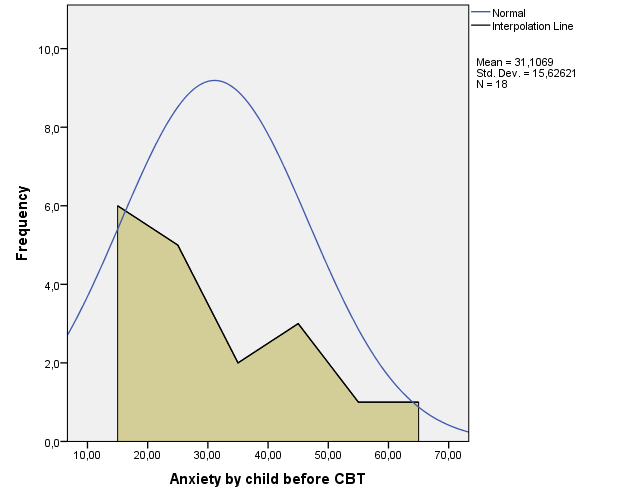
\includegraphics[width=0.8\textwidth]{STATS1B-HW4-Q5b-1}
            \caption{This (centred) histogram of the data from \texttt{anxc1} shows that it is a right-skewed distribution, with $\bar{x}=31.1069$, $s=15.62621$, and $n=18$.}
            \label{fig:hw4q5b}
        \end{figure}
        \FloatBarrier
    \end{enumerate}
\end{enumerate}

\subsection{Homework 5}
\begin{enumerate}
    \item Repeat the comparison of the QSHA scores of the first- and second-year psychology students in the homework Exercise 3 from last week, only this time use the pooled-variance $t$ test.
    \begin{enumerate}
        \item Perform the significance test and determine the $p$ value.
        \begin{framed}{\textbf{Solution}}
        Begin by computing the pooled variance:
        \begin{align}
            s_p^2 &= \frac{\brac{n_1 - 1}s^2_1 + \brac{n_2 - 1}s^2_2}{\brac{n_1 - 1} + \brac{n_2 - 1}} \\
            &= \frac{24 \times 4.89^2 + 28\times 5.65^2}{24 + 28} = \frac{1467.7204}{52} \approx 28.2254.
            \shortintertext{So our pooled standard deviation is $\sqrt{28.2254} \approx 5.313$ allowing us to compute the standard error:}
            se &= s_p \sqrt{\frac{1}{n_1} + \frac{1}{n_2}} = 5.313 \times \sqrt{\frac{1}{25} + \frac{1}{29}} \approx 1.45. \\
            \implies t &= \frac{131-127}{se} = \frac{4}{1.45} \approx 2.759 \sim t(52).
            \intertext{We can see from table $B$ that a $t$-statistic which is more extreme than 2.009 is significant at the 5\% level (noting that our null hypothesis is two-sided) for 50 degrees of freedom. In our case we have $n_1 + n_2- 2=52$ degrees of freedom, so it is not possible to directly read the critical $t$-value but we can assume that $2.759$ is a significant $t$-value. Using an online calculator, $t^*(52)=2.006647$ meaning that our $p$-value must be less than $0.05$ as it is less than our statistic. Indeed,}
            p &= \pr{\vbrac{t_{52}} > 1.952} = 0.007985.
        \end{align}
        \end{framed}
        
        \item Compute the 95\% confidence interval for the difference between the QHSA scores of first- and second-year psychology students.
        \begin{framed}{\textbf{Solution}}
        In the previous part, we calculated the critical $t$-value for 52 degrees of freedom as $2.006647$, so our 95\% CI for $\mu_d$ is
        \begin{align}
            \Bar{x}_1 - \bar{x}_2 \pm t^*_{52} \times se = 4 \pm 2.006647 \times 1.45 = 4\pm 2.91 = \brac{1.09 , 6.91}.
        \end{align}
        The probability that the true value of the parameter for the difference in means in the population lies between 1.09 and 6.91 is 0.950.
        \end{framed}
        
        \item Compare your results with the results in homework Exercise 3 of last week. How well do the results of the different two-sample $t$ procedures correspond?
        \begin{framed}{\textbf{Solution}}
        The samples are of similar (not equal) size, which accounts for how similar the Standard Errors are (1.434 for unpooled v.s. 1.45 for pooled). The main difference is the degrees of freedom used for the test: in the previous homework, we use 24 which resulted in a fatter tailed distribution, larger critical value and thus larger margin of error for the confidence interval. 
        \end{framed}
%%%%%%%%tikz here
    \end{enumerate}
    
    \item Due to a shooting incident in a Rotterdam supermarket where a member of the supermarket staff was shot, the supermarket wanted to determine whether the public thought supermarkets were safe. The following question was asked: ``Supermarkets should close at night for security reasons''. Of the 500 respondents, 156 answered with ``Yes'', and 344 with ``No''.
    \begin{enumerate}
        \item Compute the sample proportion that said ``Yes'', and estimate the standard deviation of that proportion.
        \begin{framed}{\textbf{Solution}}
        The sample proportion that said ``yes'' is the number of people who said ``yes'' divided by the total number of people in the sample:
        \begin{align}
            \Hat{\pi} &= \frac{156}{500} = 0.312.
            \intertext{The estimate for the standard deviation of the proportion (or standard error of the estimate) is given by the square root of the proportion that said ``yes'' times the proportion that said ``no'' divided by the sample size:}
            se &= \sqrt{\frac{\Hat{\pi} \brac{1-\Hat{\pi}}}{n}} = \sqrt{\frac{0.312 \times 0.688}{500}} = \sqrt{0.000429312} \approx 0.02072.
        \end{align}
        \end{framed}
        
        \item Use your answer to the previous question to find a 95\% confidence interval for the proportion people that advocate closing supermarkets at night.
        \begin{framed}{\textbf{Solution}}
        \begin{align}
            \text{95\% CI for $\pi$: } \Hat{\pi} \pm 1.96 \times se &= 0.312 \pm 1.96 \times 0.02072 \\
            &= \brac{0.2714 , 0.3526}.
        \end{align}
        The true proportion of the population that believe supermarkets should be closed at night for security reasons lies between 0.2714 and 0.3526 with probability of 0.95. As this does not constitute a majority vote, we decline to close supermarkets at night for security reasons. 
        \end{framed}
    \end{enumerate}
    
    \item A matched-pairs experiment is done that compared the taste of ``regular'' fresh coffee with the taste of Senseo coffee. Every participant tasted two unmarked cups of coffee, one of each kind of coffee. The tastings were done in a random order. Each participant was asked to tell which one of the two cups they preferred. Of the 60 participants, 26 preferred regular coffee, and 34 preferred the Senseo coffee. Assume that $p$ is the chance that a randomly taken person prefers ``regular'' fresh coffee over Senseo.
    \begin{enumerate}
        \item Test the claim that a majority of people prefer regular coffee. Note the $z$ statistic and the $p$-value.
        \begin{framed}{\textbf{Solution}}
        We will consider rejecting the assumption that there is no preference in favour of a majority of people preferring ``regular'' fresh coffee over Senseo if the $p$-value is less than our prescribed $\alpha$. We formulate our hypotheses:
        \[
        \begin{matrix}
        H_0 & : & p = 0.5 \\
        H_a & : & p>0.5.
        \end{matrix}
        \] 
        Next, we calculate the standard error of the estimate under the null hypothesis in a sample size of 60:
        \begin{align}
            se_0 &= \sqrt{\frac{p_0 \brac{1 - p_0}}{n}} = \sqrt{\frac{0.5^2}{60}} \approx 0.065.
            \intertext{Finally, we calculate our $z$-value:}
            z &= \frac{\Hat{p} - p_0}{se_0} = \frac{\sfrac{26}{60} - 0.5}{0.065} \approx -1.026.
            \intertext{Visualise this $z$-value on the standard normal distribution, and recall that \~68\% of the population data lies between $-1$ and 1. A two-sided $p$-value would be roughly $(100-68)\% = 32\%$, so the right-tailed $p$-value would be roughly $(50 + 68/2)\% = 84\%$ and the left-tailed would be roughly $(100-84)\%=16\%$. This allows us to already deduce that we will not be rejecting our null hypothesis. Keeping this in mind, we calculate the $p$-value as}
            p &= \pr{Z>-1.026}
            \shortintertext{As the standard normal distribution is symmetric about the mean of zero, we can solve this as}
            &= \pr{Z<1.026} = 0.847554,
        \end{align}
        which agrees with our theoretical calculation.
        \end{framed}
        
        \item Is this result significant, using $\alpha = 0.05$?
        \begin{framed}{\textbf{Solution}}
        $p>\alpha$, so yeah.
        \end{framed}
        
        \item Compute a 90\% confidence interval for p.
        \begin{framed}{\textbf{Solution}}
        \begin{align}
            \text{90\% CI for $p$: } \Hat{p} \pm 1.645 \times se &= \sfrac{26}{60} \pm 1.645 \sqrt{\frac{26 \times 34}{60^3}} \\
            &\approx 0.4\bar{3} \pm 1.645 \times 0.064 \\
            &= \brac{0.3281 , 0.5386}.
        \end{align}
        The true value of the chance that a randomly selected person from the population that prefers ``regular'' fresh coffee over Senseo lies between 0.3281 and 0.5386 with probability of 0.9. Note that $p_0 = 0.5$ is contained in the 90\% CI.  
        \end{framed}
        
        \item Using your two answers above, form your conclusion about whether a majority of people prefer fresh coffee.
        \begin{framed}{\textbf{Solution}}
        It appears that they do not care either way, as we do not reject the null hypothesis that the chance a randomly selected person prefers ``regular'' fresh coffee over Senseo is 50\%.
        \end{framed}
    \end{enumerate}
    
    \item Suppose that in a study on depression among children, the researchers wanted to show a relationship between the depression among children and the composition of the family. The researchers made a distinction between one- and two-parent families. The following table shows the results of the study. The variable $X$ refers to the number of children with a diagnosis of depression, and $n$ refers to the total number of families of that type.
    \FloatBarrier
    \begin{table}[h]
    \centering
    \begin{tabular}{l|c|c}
    Family type & $n$ & $X$ \\ \hline
    One-parent families & 74 & 6 \\
    Two-parent families & 226 & 13
    \end{tabular}
    \end{table}
    \FloatBarrier
    \begin{enumerate}
        \item For the one-parent families, compute the proportion of children suffering from depression.
        \begin{framed}{\textbf{Solution}}
        Let $\pi_1$ denote the proportion of children in one-parent families suffering from depression (note that this is conditional on the number of parents!!), so $\hat{\pi}_1 = \sfrac{6}{74}=0.\overline{081}\approx 0.0811$. That means that the sample proportion of children in one-parent families not suffering from depression is $(1-0.0811) = 0.\overline{918}\approx 0.9189$.
        \end{framed}
        
        \item For the two-parent families, compute the proportion of children suffering from depression.
        \begin{framed}{\textbf{Solution}}
        Let $\pi_2$ denote the proportion of children in two-parent families suffering from depression, so $\hat{\pi}_2 = \sfrac{13}{226}\approx 0.0575$. That means that the sample proportion of children in two-parent families not suffering from depression is $(1-0.0575)\approx 0.9425$.
        \end{framed}
        
        \item Compute a 95\%-confidence interval for the difference between these proportions.
        \begin{framed}{\textbf{Solution}}
        95\% CI for $\pi_1 - \pi_2$: 
        \begin{align}
            \Hat{\pi}_1 - \Hat{\pi}_2 \pm 1.96 \times \sqrt{\frac{\Hat{\pi}_1 \times \brac{1-\Hat{\pi}_1 }}{n_1} + \frac{\Hat{\pi}_2 \times \brac{1-\Hat{\pi}_2 }}{n_2}} &= 0.02356 \pm 1.96 \times \sqrt{0.001007 + 0.015488} \\
            &= 0.02356 \pm 1.96 \times 0.12843 \\
            &= \brac{-0.228 , 0.275}.
        \end{align}
        Note that we used unpooled standard error? This is because we do not assume homoskedasticity in the population as it is not plausible. 
        \end{framed}
        
        \item On the basis of your computations above, what are your conclusions regarding depression and family composition?
        \begin{framed}{\textbf{Solution}}
        The true value of the difference between the proportions lies near and about zero, and ranges from $-0.228$ to $0.275$ with probability 0.95. This allows us to conclude that there is no real difference in the chances a child will suffer from depression whether they have one- or two-parent families. You could loosely conclude that a child who has a one-parent family is not more likely to develop depression than a child who has two parents, and thus single parents do a ``good job'' at ensuring their childrens' happiness.
        \end{framed}
    \end{enumerate}
    
    \item Eisses and Kluiter's did a study on depression symptoms among nursing home residents [Eisses and Kluiter, 2002]. The researchers found that the percentage of elderly people undergoing treatment for depression is lower in Drenthe than in the rest of the Netherlands. It was suspected that the staff in Drenthe nursing homes needed better training to detect depression symptoms, so a study was conducted to evaluate the effect of training. Six nursing homes took part in the study. The staff from the nursing homes were assigned to either a control condition (no training) or an experimental condition (training to detect depression symptoms). Three nursing homes were assigned to the control condition, and three to the experimental condition.
    \\
    Before and after the training, the residents of the nursing home were interviewed by an independent clinical psychologist. Based on the reports of individual residents, the psychologist determined whether that resident was suffering from depression. Eisses and Kluiter used the independent psychologist's diagnoses to compare to the staff's diagnoses, but in this practicum we will only analyze the report of the independent psychologist.
    \\
    Open the file \texttt{5 - Depression Diagnosis.sav}.
    \FloatBarrier
    \begin{table}[h]
    \centering
    \begin{tabular}{l|l}
    \textbf{Variable} & \textbf{Description} \\
    \texttt{participant} & Participant number \\
    \texttt{exp} & 1=control group, 2=experimental group \\
    \texttt{depdiaB} & depression diagnosis before staff training: 1=yes, 2=no, 9=missing \\
    \texttt{depdiaA} & depression diagnosis after staff training: 1=yes, 2=no, 9=missing
    \end{tabular}
    \end{table}
    \FloatBarrier
    Some data is missing, due to the fact that the residents moved between interviews.
    \\
    One question of interest is: what proportion of residents of nursing homes in Drenthe suffer from depression?
    \begin{enumerate}
        \item To answer this question would you use the scores on the pre-training measure, the post-training measure, or both? Explain your answer.
        \begin{framed}{\textbf{Solution}}
        The scores on the pre-training measure would be most useful in answering this question, as we do not want that the additional staff training provides a confounding variable for us to solve. By doing so, we negate the allocation to control or experimental group and can simply estimate the proportion of residents of nursing homes in Drenthe suffering from depression. 
        \end{framed}
        
        \item Compute the proportion of residents suffering from depression before the training. Look closely at the frequency table. How many residents are diagnosed as depressed before the training? What percent is depressed?
        \begin{framed}{\textbf{Solution}}
        The first thing to notice is that 28 of 701 participants have missing data, so keeping that adjustment in mind the sample proportion is 0.045 even though there are 30 residents with depression in total. With respect to the total 4.3\% have depression, and when accounting for the missing data we have 4.5\%. The frequency table is given in \Cref{tab:hw5q5b}.
        \end{framed}
        \begin{figure}[h]
            \centering
            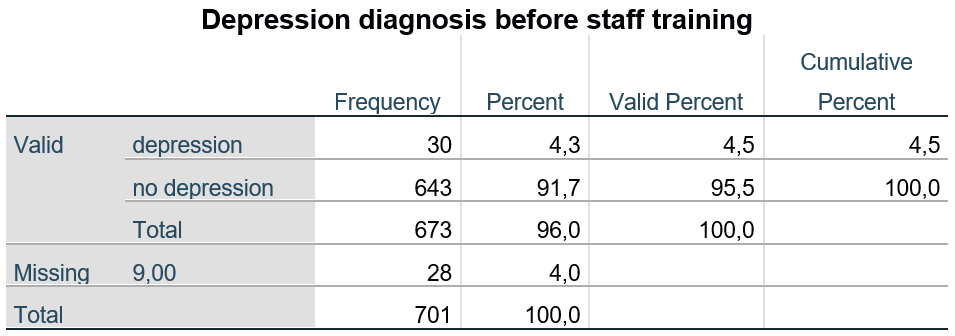
\includegraphics[width=0.68\linewidth]{STATS1BHW5Q5b-tabonly.png}
            \caption{SPSS frequency table output for the proportion of residents of nursing homes in Drenthe suffering from depression prior to initiating staff training in detecting symptoms of depression.}
            \label{tab:hw5q5b}
        \end{figure}
    \end{enumerate}
    These data will be used again in next week’s practicum.
\end{enumerate}

\subsection{Homework 6}
\begin{enumerate}
    \item Appleton, French and Vanderpump [Appleton et al., 1996] reported the results of a large epidemiological study of women in Great Britain. In the beginning of the 1970s, many women in Great Britain were asked about their health and health-related habits. Twenty years later, the women were contacted again to determine who had lived and who died. The table below shows the results.
    \FloatBarrier
    \begin{table}[h]
        \centering
        \begin{tabular}{c|cc}
             {} & Smoker & Non-smoker \\ \hline
             Dead & 139 & 230 \\
             Alive & 443 & 502 \\ \hline 
             Total & 582 & 732
        \end{tabular}
    \end{table}
    \FloatBarrier
    \begin{enumerate}
        \item Analyze the data, using plots and descriptive statistics. Use SPSS and/or R (hint: type in ``?prop.test'' in R and pay attention to the examples below) for your analysis. Describe what you did and sketch a copy of any informative plot you made.
        \begin{framed}{\textbf{Solution}}
        For obvious reasons, let's denote ``success'' as being alive, and failure as being ``dead'' with respect to table 8.6 from Agresti. So we have $\hat{\pi}_1 = 443/582 \approx 0.76117 $, $\hat{\pi}_2 = 502/732 \approx 0.68579 $, $\hat{\pi} = (443+502)/(582+732) = 945/1314 \approx 0.71918$ and $se_0 = \sqrt{\hat{\pi}\brac{1 - \hat{\pi}}\brac{\sfrac{1}{n_1} + \sfrac{1}{n_2}}} = \sqrt{0.71918\brac{1 - 0.71918}\brac{\sfrac{1}{582} + \sfrac{1}{732}}} \approx 0.02496$, which results in the $z$-statistic $\brac{\hat{\pi}_1 - \hat{\pi}_2}/se_0 = (0.76117 - 0.68579)/0.02496 \approx 3.02$. This $z$-statistic already indicates that $p<\alpha = 0.05$ and we will reject the null hypothesis ($H_0: \pi_1 = \pi_2$) and squaring gives $z^2=9.12$. 
        If you're using \texttt{R}, input the following code:\\
        \texttt{alive <- c(443,502)} \\
        \texttt{total <- c(582,732)} \\
        \texttt{prop.test(alive,total)} 
        \begin{center}
            \texttt{2-sample test for equality of proportions with continuity correction} 
        \end{center}
        \texttt{\quad data:  alive out of total \\
        \quad X-squared = 8.7515, df = 1, p-value = 0.003093 \\
        \quad alternative hypothesis: two.sided \\
        \quad 95 percent confidence interval: \\
        \quad  0.02555629 0.12519578 \\
        \quad sample estimates: \\
        \quad    prop 1    prop 2  \\
        \quad 0.7611684 0.6857923} \\
        You can use a bar graph of the sample percentages to display this information. 
        \end{framed}
        
        
        \item Based on the data in the table, what do you conclude?
        \begin{framed}{\textbf{Solution}}
        We assume that the population variables $\pi_1$ and $\pi_2$ are independent, i.e. smoking does not negatively influence the health of a woman (during that time period), and would expect that $\hat{\pi}_1 \approx \hat{\pi}_2$ in any sample from said population. 
        \end{framed}
        
    \FloatBarrier
    \begin{table}[h]
        \centering
        \begin{tabular}{c|cc}
             {} & Smoker & Non-smoker \\ \hline
             Dead & 23.88\% & 31.42\% \\
             Alive & 76.12\% & 68.58\% \\ \hline 
             Total & 100\% & 100\%
        \end{tabular}
    \end{table}
    \FloatBarrier
    \end{enumerate}
    
    \item In a longitudinal study of sexual orientation by [Golombok and Tasker, 1996], children of homosexual mothers were compared to children of heterosexual single mothers. The researchers asked the children about their sexual orientation when they were about 24 years old. The following table shows the children's sexual orientations as a function of the mothers' sexual orientations.
    \FloatBarrier
    \begin{table}[h]
        \centering
        \begin{tabular}{ll|cc}
            &  & \multicolumn{2}{c}{Mother} \\
            &  & Homosexual & Heterosexual \\ \hline 
            \multicolumn{1}{r}{\multirow{2}{*}{Child}} & Homosexual/bisexual & 2 (Expected: \underline{$1.1\bar{1}$}) & 0 (Expected: \underline{$0.8\bar{8}$}) \\
            \multicolumn{1}{r}{} & Heterosexual & 23 (Expected: \underline{$23.8\bar{8}$}) & 20 (Expected: \underline{$19.1\bar{1}$}) \\ \hline
            & Total & 25 & 20
        \end{tabular}
    \end{table}
    \FloatBarrier
    The SPSS file with these data is \texttt{6 - Golombok and Tasker.sav}.
    \begin{enumerate}
        \item Compute the expected frequencies under the assumption that the two factors are independent with SPSS. Note them in the previous table.
        \begin{framed}{\textbf{Solution}}
        You can calculate the expected frequencies using Bayes' Rule for Independence. First we denote $M_H$ as the event that the mother is homosexual and $M_S$ as the event that the mother is heterosexual. Similarly, $C_H$ denotes the event that the child is homo/bisexual and $C_S$ denotes the event that the child is heterosexual. The marginal probabilities can be found by adding the row or column frequencies and dividing by the sample size, e.g. $\pr{M_H} = 25/45$.
        \begin{align}
            \pr{A \cap B} &= \pr{A} \times \pr{B} .
            \intertext{The above formula is Bayes' Rule for Independence.}
            \implies \pr{M_H \cap C_H} &= \pr{M_H} \times \pr{C_H} = \frac{25}{45} \times \frac{2+0}{45} = \frac{50}{45^2} \approx 2.47\%. 
            \intertext{Assuming that the two factors are independent, we find that there is a 2.47\% chance that a homosexual mother will have a child that is homo/bisexual as well. We now know the probability of such an event, so multiplying it by the sample size will give the expected value. }
            \implies \E\brac{M_H \cap C_H} &= 45 \times 2.47\% = \frac{50}{45} = 1.1\bar{1}.
            \intertext{The expected number of homo/bisexual children who also have a homosexual mother is less than the observed value of 2, and is 1.11. The other probabilities are calculated in the following way:}
            \pr{M_S \cap C_H} &= \pr{M_S} \times \pr{C_H} = \frac{20}{45} \times \frac{2+0}{45} = \frac{40}{45^2} \approx 1.98\%. \\
            \pr{M_H \cap C_S} &= \pr{M_H} \times \pr{C_S} = \frac{25}{45} \times \frac{23+20}{45} = \frac{1075}{45^2} \approx 53.09\%. \\
            \pr{M_S \cap C_S} &= \pr{M_S} \times \pr{C_S} = \frac{20}{45} \times \frac{23+20}{45} = \frac{860}{45^2} \approx 42.47\%.
            \intertext{Which gives us the following expected values:}
            \implies \E\brac{M_S \cap C_H} &= 45 \times 1.98\% = \frac{40}{45} = 0.8\bar{8}. \\
            \E\brac{M_H \cap C_S} &= 45 \times 53.09\% = \frac{1075}{45} = 23.8\bar{8}. \\
            \E\brac{M_S \cap C_S} &= 45 \times 42.47\% = \frac{860}{45} = 19.1\bar{1}. 
        \end{align}
        \end{framed}
        
        \item Is a $\chi^2$ test appropriate for these data? Why or why not?
        \begin{framed}{\textbf{Solution}}
        No. We need the expected frequencies in each cell to be at least 5, or at least 10 for df=1.
        \end{framed}
        
        \item Use SPSS to perform the $\chi^2$ test and examine the output. Note it below. Notice that SPSS informs you about the number of cells with a frequency below five.
        \begin{framed}{\textbf{Solution}}
        
        \begin{align}
            \chi^2 &= \sum_{i=1}^k\frac{\brac{f_{0,i} - f_{e,i}}^2}{f_{e,i}}
            \shortintertext{$f_{0,i}$ denotes the \textit{observed} frequency and $f_{e,i}$ denotes the \textit{expected} frequency in cell $i$, where $i$ is the number of rows $r$ times the number of columns $c$ so here $i=2 \times 2=4$.}
            &=\frac{\brac{2 - 1.11}^2}{1.11} + \frac{\brac{0 - 0.89}^2}{0.89} + \frac{\brac{23 - 23.89}^2}{23.89} + \frac{\brac{20 - 19.11}^2}{19.11} \\
            &= \frac{0.89^2}{1.11} + \frac{0.89^2}{0.89} + \frac{0.89^2}{23.89} + \frac{0.89^2}{19.11}. \\
            &\approx 1.678. 
            \shortintertext{The $p$-value is calculated as follows:}
            p &= \pr{\chi^2_1 > 1.678} = 0.19519.
        \end{align}
        You can enter the following into R to achieve the same output: \\
        \texttt{x <- matrix(c(2,23,0,20), nrow=2) \\
         chisq.test(x,correct=FALSE)} 
         \begin{center}
             \texttt{Pearson's Chi-squared test}
         \end{center}
        \texttt{data:  x \\
        X-squared = 1.6744, df = 1, p-value = 0.1957} \\
        The use of \texttt{correct=FALSE} removes Yates' continuity correction. \\
        As $df = (r-1)\times (c-1) = 1$, we can also look at $z^2$: first calculate the standard error under the null hypothesis of $\pi_1 = \pi_2$:
        \begin{align}
            \hat{\pi} &= \frac{2}{45} \approx 0.0\bar{4}. \\
            \implies se_0^2 &= \hat{\pi}\brac{1-\hat{\pi}}\brac{\frac{1}{n_1} + \frac{1}{n_2}} \\
            &= 0.0\bar{4}\times 0.9\bar{5} \brac{\frac{1}{25} + \frac{1}{20}} = \frac{2 \times 43}{45^2} \times \frac{9}{100} = \frac{43}{11250} \approx 0.0038\bar{2}. \\
            \implies z^2 &= \frac{\brac{\hat{\pi}_1 - \hat{\pi}_2}^2}{se_0^2} \\
            &= \frac{\brac{\sfrac{2}{25} - \sfrac{0}{20}}^2}{0.0038222} = \frac{72}{43} \approx 1.6744.
            \intertext{We would have a significant result if the statistic $z^2$ is more extreme than $1.96^2 = 3.8416$ for $\alpha=0.05$, which it isn't. The $p$-value is calculated as follows:}
            p &= \pr{\chi^2_1 > 1.674} = 0.195724.
        \end{align}
        Neither $p$-value is significant at $\alpha = 0.05$ level - we do not reject the null hypothesis that they are independent
        \end{framed}
        
        \item The SPSS output also yields the result of Fisher's exact test. Note the result of this test, along with the relevant statistics.
        \begin{framed}{\textbf{Solution}}
        You can calculate this yourself using the hypergeometric distribution:
        \begin{align}
             p_1 &= \frac{2! 43! 25! 20!}{2!0!23!20!45!} \approx 0.303030
            \intertext{As 2 is the greatest possible number for this cell, keeping the marginal frequencies the same (other possibilities are 1 and 0), this is the right-tailed $p$-value. Next, you need to calculate the $p$-values for different extremes \textit{without altering the marginal frequencies}, i.e. altering only the cell frequencies:}
            p_2 &= \frac{2! 43! 25! 20!}{1!1!24!19!45!} \approx 0.50505.  \\
            p_3 &= \frac{2! 43! 25! 20!}{0!2!25!18!45!} \approx 0.191919.
            \intertext{If you added all the $p$-values together, you would get the left-tailed $p$-value\footnotemark. If you add together the $p$-values of all combinations that have lower probabilities than that of the observed data (so $p$-values less than $0.303030 = p_1$), you get the two-tailed $p$-value. The only $p$-value that is smaller than $p_1$ is $p_3$ (so for $\cbrac{(0,2), (25,18)}$), hence we add $p_1$ and $p_3$ together to get the two-tailed $p$-value:}
            p &= 0.30303 + 0.191919 = 0.494949.
        \end{align}
        You can do this in R: \\
        \texttt{x <- matrix(c(2,23,0,20), nrow=2) \\
         exact2x2(x,tsmethod="minlike")}
         \begin{center}
             \texttt{Two-sided Fisher's Exact Test (usual method using minimum likelihood)}
         \end{center}
         \texttt{data:  x\\
         p-value = 0.4949\\
         alternative hypothesis: true odds ratio is not equal to 1\\
         95 percent confidence interval:\\
         0.2316 \quad Inf\\
         sample estimates:\\
         odds ratio \\
        ${}$ \quad Inf} \\
        Note that the confidence interval given is unbounded as it tends to $\infty$? This is because of the inclusion of the zero in our table: the odds ratio is $OR = (2/23)/(0/20) = (2/23) \times (20/0) = \infty$ and everyone knows you can't divide by zero. The computation of the 95\% Confidence Interval for the odds ratio is as follows:
        \begin{align}
            se_{\ln{\brac{OR}}} &= \sqrt{\frac{1}{2} + \frac{1}{0} + \frac{1}{23} + \frac{1}{20}} = \sqrt{\infty}. 
            \shortintertext{95\% CI for odds ratio:}
            \exp{\cbrac{\ln{\brac{OR}} \pm 1.96 \times se_{\ln{\brac{OR}}}}} &= \exp{\cbrac{\ln{\brac{\infty}} \pm 1.96 \times \sqrt{\infty}}} \\
            &= \brac{\infty \times e^{-1.96 \times \sqrt{\infty}} , \infty \times e^{1.96 \times \sqrt{\infty}}} \\
            &= \brac{0.2316 , \infty}.
        \end{align}
        This issue is not present when you don't have zero values in the table - a rearrangement of the columns does not aid us any further as we still have the zero in the odds ratio and the computation of the standard error. 
        \end{framed}
        \footnotetext{You can play around with the following applet to see what I mean with left- and right-tailed $p$-values: \url{https://istats.shinyapps.io/FisherExact/}.}
        
        \item Fisher's exact test was developed by the famous statistician R.A. Fisher. It is designed to test the same null hypothesis as the $\chi^2$ test, but it does not have the same problems with low cell counts that the $\chi^2$ test has. In this class you will not learn the details of how to compute the test by hand, but notice that SPSS gives a $p$ value for the test every time you compute a $\chi^2$ test. What do you conclude on the basis of Fisher's exact test?
        \begin{framed}{\textbf{Solution}}
        Fisher's exact test starts by computing the probabilities of \textit{all possible outcomes which do not alter the marginal frequencies} ($p_1$, $p_2$ and $p_3$), and adding all of these equates to the probability of all events, thus equals 1. For this reason, it is called \textit{exact} as you can exactly calculate the probability of any event using the actual (hypergeometric) sampling distribution rather than a normal approximation. The sampling distribution is not symmetric for low $n$, meaning that left-, right-, and two-tailed $p$-values do not add up to 1.
        \end{framed}
        
        \item It is also true that confidence intervals computed using small sample sizes can be quite inaccurate. What implications does this have for designing studies using two-way data?
        \begin{framed}{\textbf{Solution}}
        They are inaccurate due the lack of central tendency and presence of skew, also having a zero in the computation of the odds ratio (and therefore confidence interval) is really hard to work with, as written above. 
        \end{framed}
    \end{enumerate}
\end{enumerate}

\end{document}